%%%%%%%%%%%%%%%%%%%%%%%%%%%%%%%%%%%%%%%%%
% Short Sectioned Assignment LaTeX Template Version 1.0 (5/5/12)
% This template has been downloaded from: http://www.LaTeXTemplates.com
% Original author:  Frits Wenneker (http://www.howtotex.com)
% License: CC BY-NC-SA 3.0 (http://creativecommons.org/licenses/by-nc-sa/3.0/)
%%%%%%%%%%%%%%%%%%%%%%%%%%%%%%%%%%%%%%%%%

%----------------------------------------------------------------------------------------
%	PACKAGES AND OTHER DOCUMENT CONFIGURATIONS
%----------------------------------------------------------------------------------------

\documentclass[paper=a4, fontsize=11pt]{scrartcl} % A4 paper and 11pt font size

% ---- Entrada y salida de texto -----

\usepackage[T1]{fontenc} % Use 8-bit encoding that has 256 glyphs
\usepackage[utf8]{inputenc}
%\usepackage{fourier} % Use the Adobe Utopia font for the document - comment this line to return to the LaTeX default

% ---- Idioma --------

\usepackage[spanish, es-tabla]{babel} % Selecciona el español para palabras introducidas automáticamente, p.ej. "septiembre" en la fecha y especifica que se use la palabra Tabla en vez de Cuadro

% ---- Otros paquetes ----

\usepackage{url} % ,href} %para incluir URLs e hipervínculos dentro del texto (aunque hay que instalar href)
\usepackage{amsmath,amsfonts,amsthm} % Math packages
%\usepackage{graphics,graphicx, floatrow} %para incluir imágenes y notas en las imágenes
\usepackage{graphics,graphicx, float} %para incluir imágenes y colocarlas
% Para hacer cuadros
\usepackage{tcolorbox}
% Para hacer uso de párrafos
\usepackage{parskip}
\usepackage{hyperref}
\usepackage{vmargin}
\setpapersize{A4}
\setmargins{2.5cm}       % margen izquierdo
{1.5cm}                        % margen superior
{16.5cm}                      % anchura del texto
{23.42cm}                    % altura del texto
{10pt}                           % altura de los encabezados
{1cm}                           % espacio entre el texto y los encabezados
{0pt}                             % altura del pie de página
{2cm}                           % espacio entre el texto y el pie de página
% Para hacer tablas comlejas
%\usepackage{multirow}
%\usepackage{threeparttable}

%\usepackage{sectsty} % Allows customizing section commands
%\allsectionsfont{\centering \normalfont\scshape} % Make all sections centered, the default font and small caps

\usepackage{fancyhdr} % Custom headers and footers
\pagestyle{fancyplain} % Makes all pages in the document conform to the custom headers and footers
\fancyhead{} % No page header - if you want one, create it in the same way as the footers below
\fancyfoot[L]{Mario López González 3ºB} % Empty left footer
\fancyfoot[C]{} % Empty center footer
\fancyfoot[R]{\thepage} % Page numbering for right footer
\renewcommand{\headrulewidth}{0pt} % Remove header underlines
\renewcommand{\footrulewidth}{0pt} % Remove footer underlines
\setlength{\headheight}{13.6pt} % Customize the height of the header

\numberwithin{equation}{section} % Number equations within sections (i.e. 1.1, 1.2, 2.1, 2.2 instead of 1, 2, 3, 4)
\numberwithin{figure}{section} % Number figures within sections (i.e. 1.1, 1.2, 2.1, 2.2 instead of 1, 2, 3, 4)
\numberwithin{table}{section} % Number tables within sections (i.e. 1.1, 1.2, 2.1, 2.2 instead of 1, 2, 3, 4)

\setlength\parindent{0pt} % Removes all indentation from paragraphs - comment this line for an assignment with lots of text

\newcommand{\horrule}[1]{\rule{\linewidth}{#1}} % Create horizontal rule command with 1 argument of height


\title{	
\normalfont \normalsize 
\textsc{\textbf{Ingeniería de Servidores (2021-2022)} \\ Grado en Ingeniería Informática \\ Universidad de Granada} \\ [25pt] % Your university, school and/or department name(s)
\horrule{0.5pt} \\[0.4cm] % Thin top horizontal rule
\huge Memoria Práctica 3 \\ % The assignment title
\horrule{2pt} \\[0.5cm] % Thick bottom horizontal rule
}

\author{Mario López González} % Nombre y apellidos

\date{\normalsize\today} % Incluye la fecha actual

%----------------------------------------------------------------------------------------
% DOCUMENTO
%----------------------------------------------------------------------------------------

\begin{document}

\maketitle % Muestra el Título

\begin{figure}[H]
    \centering
    
\includegraphics[scale=0.175]{images/server.jpg}
    \label{fig:server}
\end{figure}

\newpage %inserta un salto de página

\tableofcontents % para generar el índice de contenidos
\listoffigures % para generar el índice de imágenes

%%%%%%%%%%%%%%%%%%%%%%%%%%%%%%%%%%%%%%%%%%%%%%%%% 
% Apartado para la instalación en Ubuntu Server %
%%%%%%%%%%%%%%%%%%%%%%%%%%%%%%%%%%%%%%%%%%%%%%%%%
\newpage
\section{Instalación de Zabbix}
\subsection{Instalación de Zabbix en Ubuntu Server}
\subsubsection{Descargar paquetes de Zabbix 5.0}

    Vamos a descargar los paquetes de Zabbix, para ello entramos en su web oficial, \href{https://www.zabbix.com/download}{Zabbix.com}, y 
    seleccionamos los siguientes parámetros ya que son los que se ajustan a nuestras necesidades.
        
    \begin{figure}[H]
        \centering
        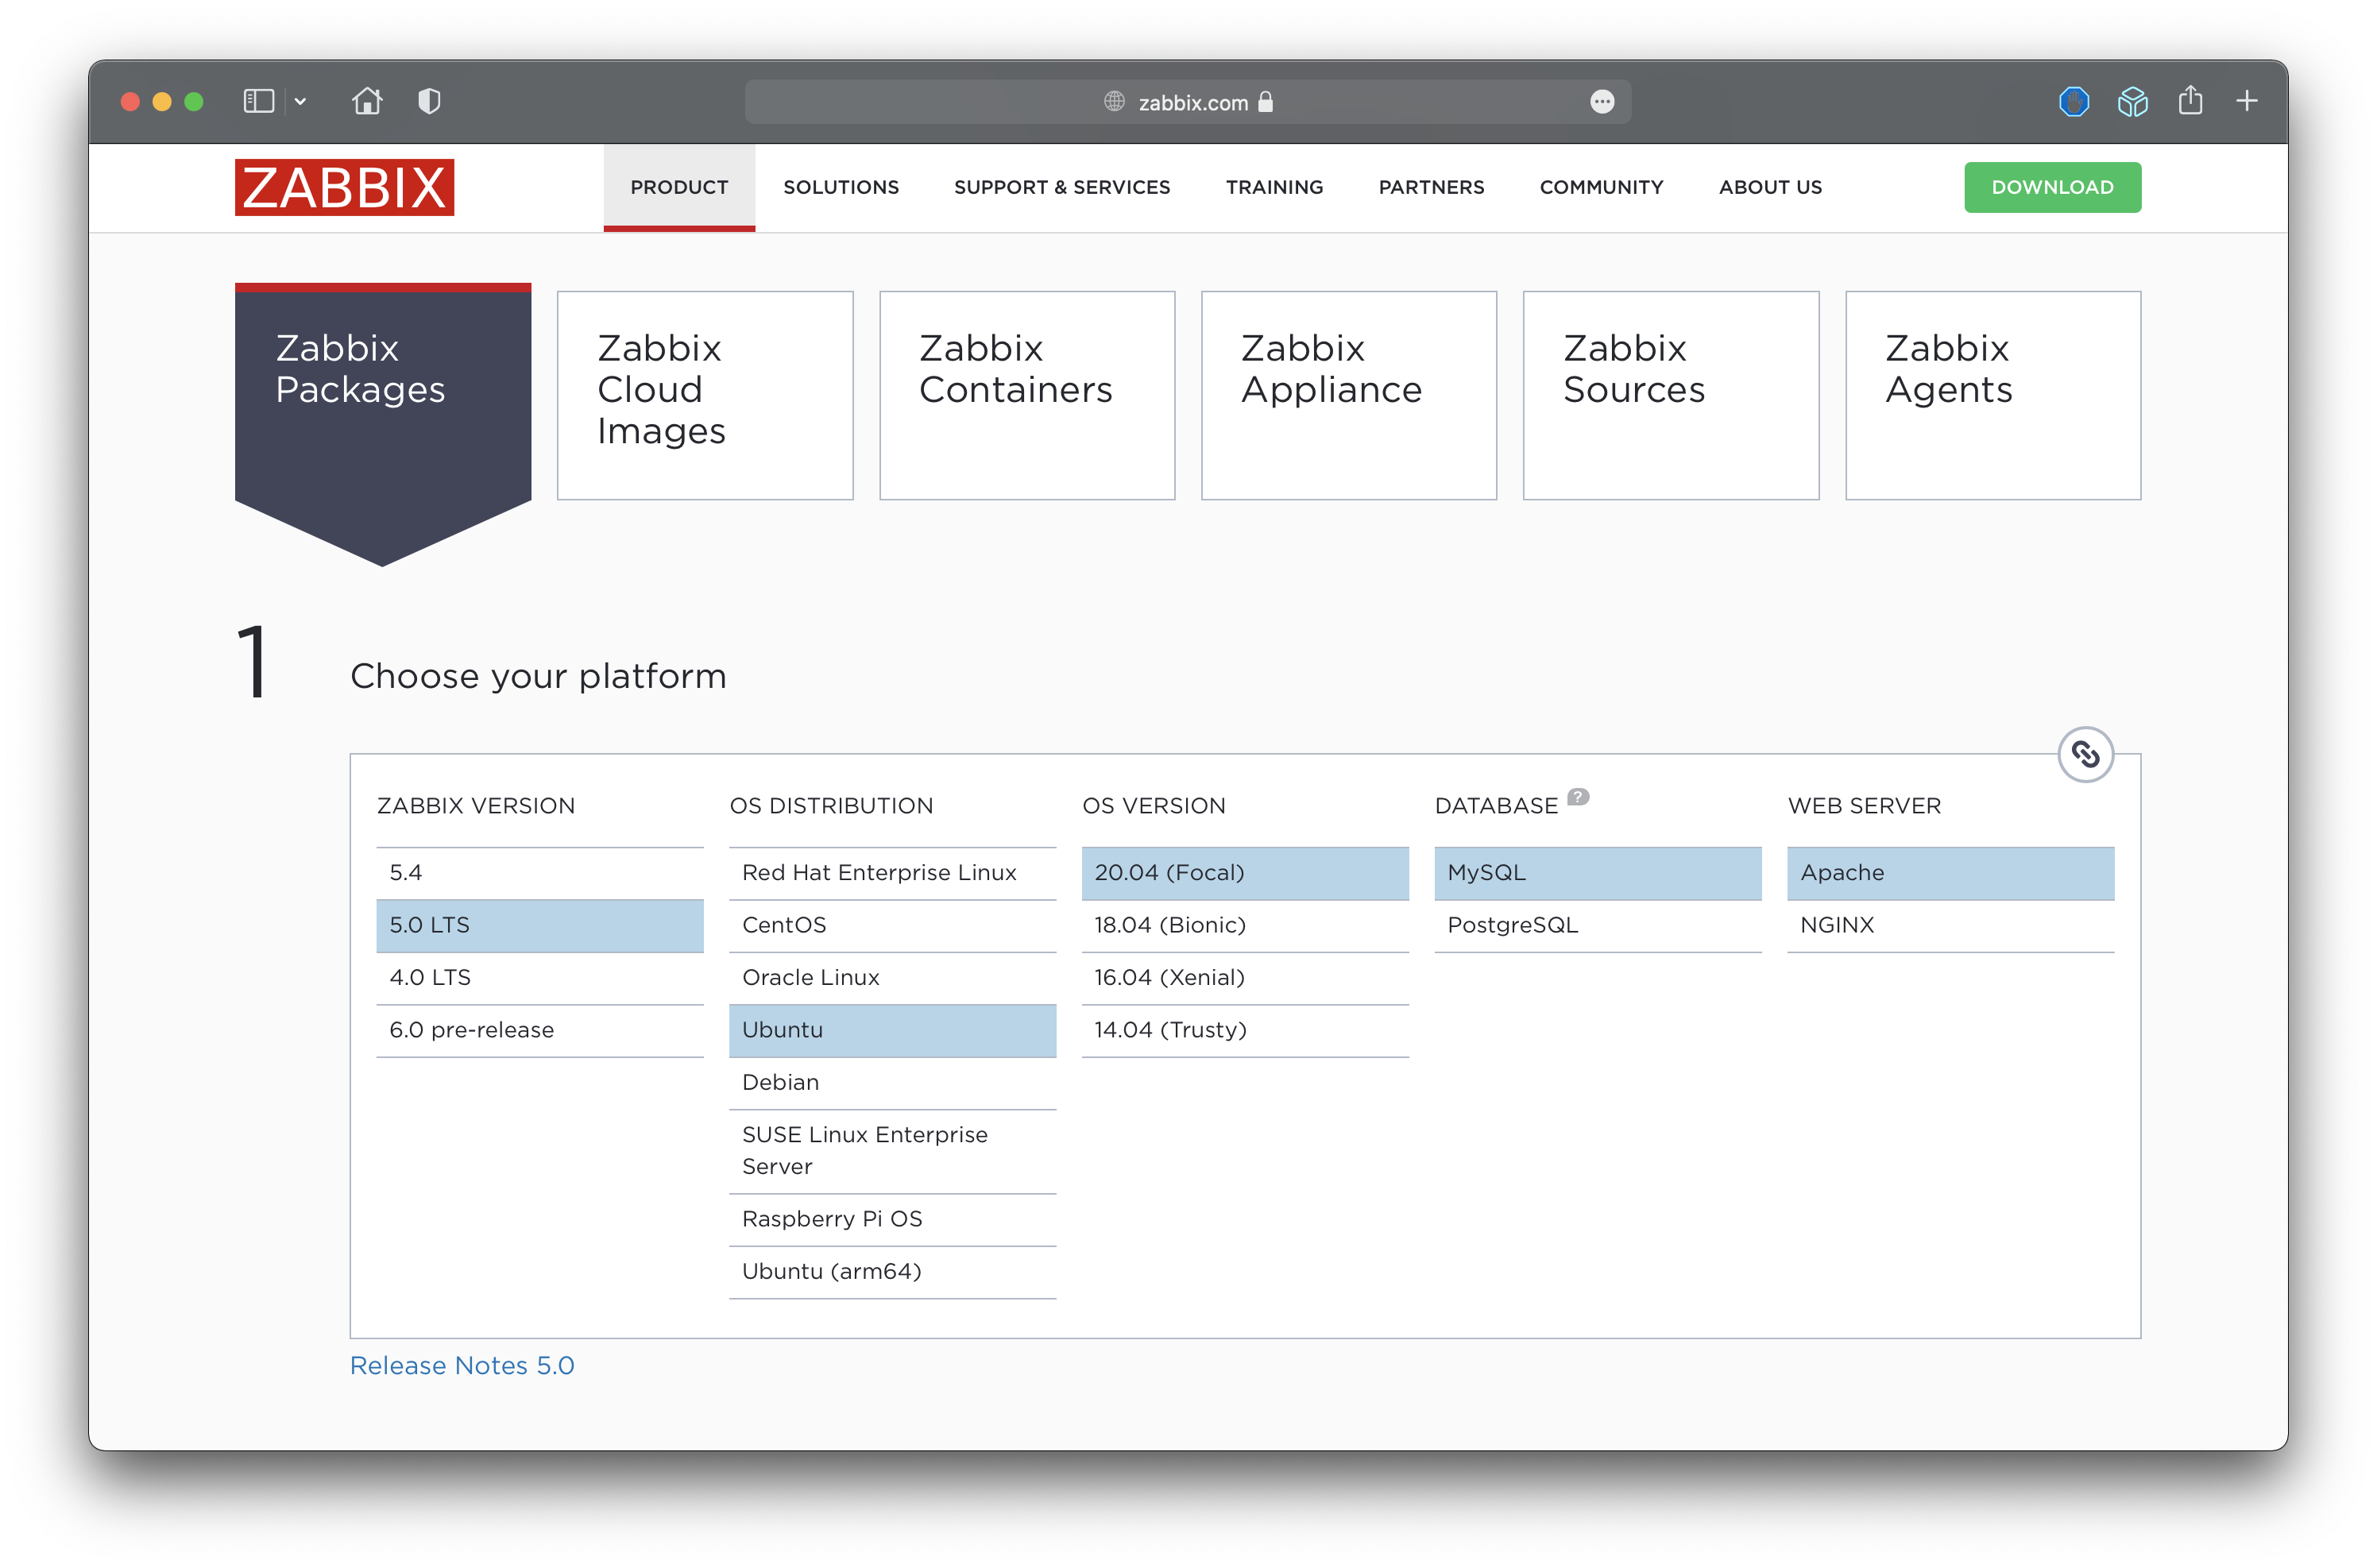
\includegraphics[scale=0.3]{images/zabbix_official.png}
        \caption{Descargar Zabbix desde paquetes}
        \label{fig:zabbix_official}
    \end{figure}

    Lo primero que debemos hacer es descargar los paquetes correspondientes a Zabbix 5.0 desde su repositorio oficial con el comando \textbf{\emph{wget}}. 
        \begin{tcolorbox}[colback=black!10, halign=left]
            \$ wget https://repo.zabbix.com/zabbix/5.0/ubuntu/pool/main/z/zabbix-release/zabbix-release\_5.0-1+focal\_all.deb
        \end{tcolorbox}

    Una vez descargado, lo instalamos el repositorio con el comando \textbf{\emph{dpkg}}.
        \begin{tcolorbox}[colback=black!10, halign=left]
            \$ sudo dpkg -i zabbix-release\_5.0-1+focal\_all.deb
        \end{tcolorbox}

    Por último actualizamos la lista de paquetes disponibles y sus versiones.
        \begin{tcolorbox}[colback=black!10, halign=left]
            \$ sudo apt update
        \end{tcolorbox}

    \newpage
    \subsubsection{Instalar Zabbix}

    Ya tenemos todos los paquetes descargados y actualizados, por lo tanto, lo siquiente que indica la web es que hay que instalar Zabbix server, frontend
    y agent con el comando \textbf{\emph{apt install}}.
        \begin{tcolorbox}[colback=black!10, halign=left]
            \$ sudo apt install zabbix-server-mysql zabbix-frontend-php zabbix-apache-conf zabbix-agent
        \end{tcolorbox}
    
    \subsubsection{Crear base de datos inicial}
    Antes de crear la base de datos inicial debemos estar seguros de que el sistema está encendido y funcionando. Una vez hechas las comprobaciones previas,
    pasamos a crear la base de datos. Para ello ingresamos en el asistente de mysql.
        \begin{tcolorbox}[colback=black!10, halign=left]
            \$ sudo mysql -u root -p

            \emph{Ingresamos la contraseña para ingresar en la base de datos (ISE)}
        \end{tcolorbox}

    Una vez dentro del asistente ejecutamos los siguientes comandos en PostgreSQL:
        \begin{tcolorbox}[colback=black!10, halign=left]
            mysql> create database zabbix character set utf8 collate utf8\_bin;

            mysql> create user zabbix@localhost identified by 'ISE';

            mysql> grant all privileges on zabbix.* to zabbix@localhost;

            mysql> quit;
        \end{tcolorbox}

    Definimos la nueva contraseña creada con el siguiente comando y escribimos la contraseña.
        \begin{tcolorbox}[colback=black!10, halign=left]
            \$ sudo zcat /usr/share/doc/zabbix-server-mysql*/create.sql.gz | mysql -uzabbix -p zabbix
            \emph{Ingresamos la contraseña (ISE)}
        \end{tcolorbox}

    \subsubsection{Configurar la base de datos de Zabbix server}
    Editamos el fichero que se encuentra en la ruta \textbf{/etc/zabbix/zabbix\_server.conf}, descomentamos el parámetro \textbf{\emph{DBPassword}} y le
    asignamos el valor \textbf{\emph{ISE}}:
    \begin{figure}[H]
        \centering
        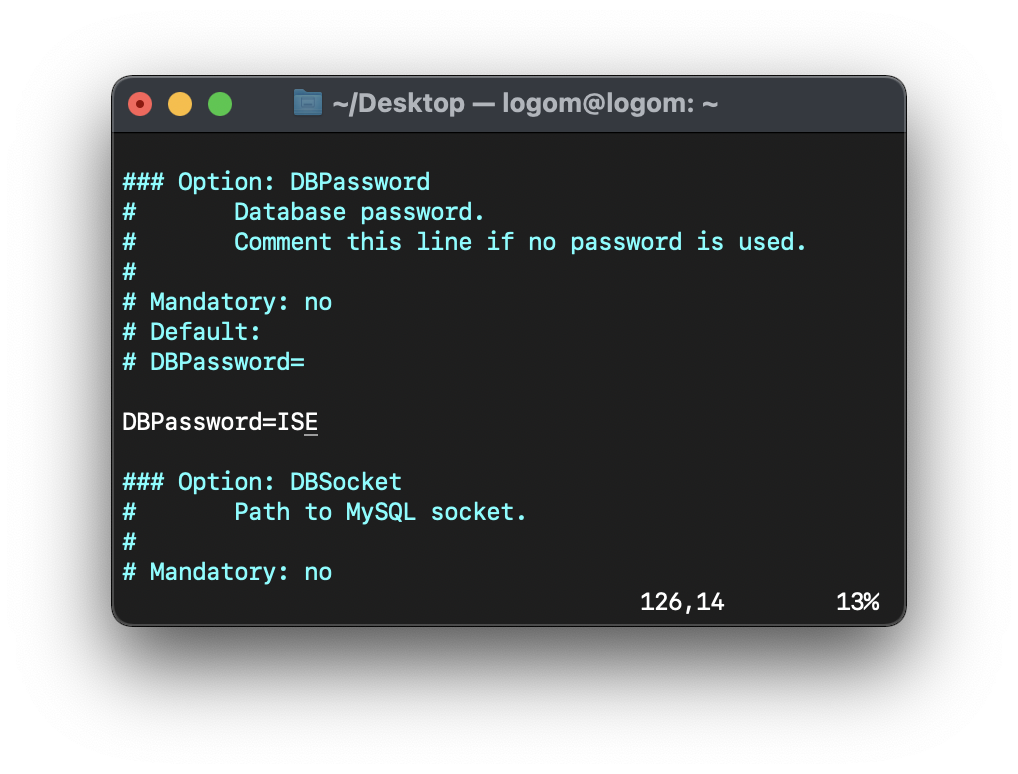
\includegraphics[scale=0.4]{images/zabbix_server_conf.png}
        \caption{Configuración base de datos}
        \label{fig:zabbix_conf}
    \end{figure}

    \subsubsection{Configurar el PHP del frontend de Zabbix}
    Editamos el fichero que se encuentra en la ruta \textbf{/etc/zabbix/apache.conf}y modificamos el parámetro comentado \textbf{\emph{php\_value date.timezone}}
    reemplazando Riga por Madrid para que se muestre la hora de forma correcta.
    \begin{figure}[H]
        \centering
        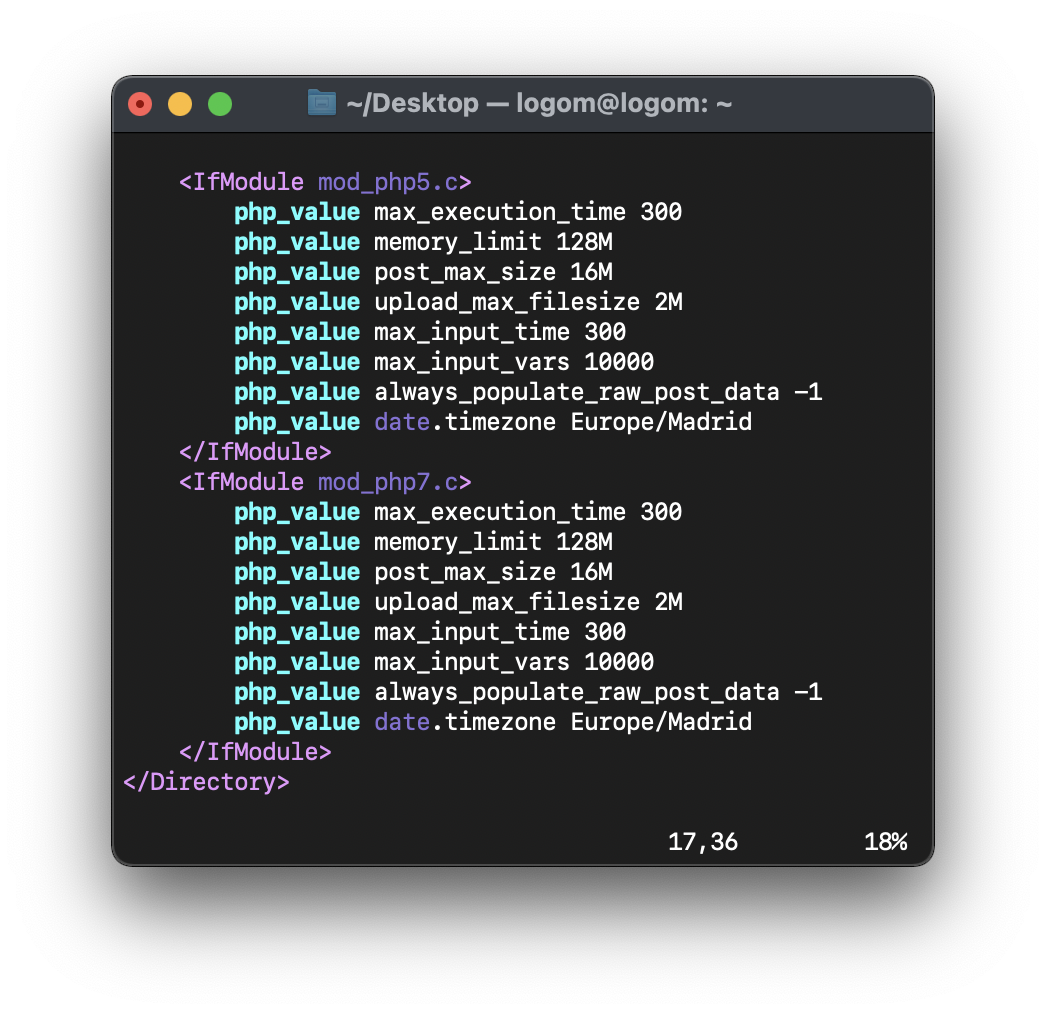
\includegraphics[scale=0.5]{images/apache_conf.png}
        \caption{Configuración base de datos}
        \label{fig:apache_conf}
    \end{figure}

    \subsubsection{Configurar los servicios}
    Reiniciamos los servicios \textbf{\emph{zabbix-server}}, \textbf{\emph{zabbix-agent}} y \textbf{\emph{apache2}} para que se actualicen los cambios realizados.
        \begin{tcolorbox}[colback=black!10, halign=left]
            \$ sudo systemctl restart zabbix-server zabbix-agent apache2
        \end{tcolorbox}

    Habilitamos los servicios anteriores para que se enciendan cuando arranque el sistema.
        \begin{tcolorbox}[colback=black!10, halign=left]
            \$ sudo systemctl enable zabbix-server zabbix-agent apache2
        \end{tcolorbox}

    \subsubsection{Habilitar el puerto de escucha}
    Habilitamos el puerto de escucha que usa por defecto Zabbix para que el firewall no lo bloquee.
        \begin{tcolorbox}[colback=black!10, halign=left]
            \$ sudo ufw allow 10051/tcp
        \end{tcolorbox}

    \subsubsection{Habilitar el puerto de escucha}
    Editamos el fichero \textbf{/etc/zabbix/zabbix\_agentd.conf} cambiando las IP asignadas a las variables Server y ServerActive por la IP de la máquina que actuará
    de servidor \textbf{(192.168.56.105)} y reiniciamos el servicio \textbf{\emph{zabbix-agent}} para que se apliquen los cambios.
        \begin{figure}[H]
            \centering
            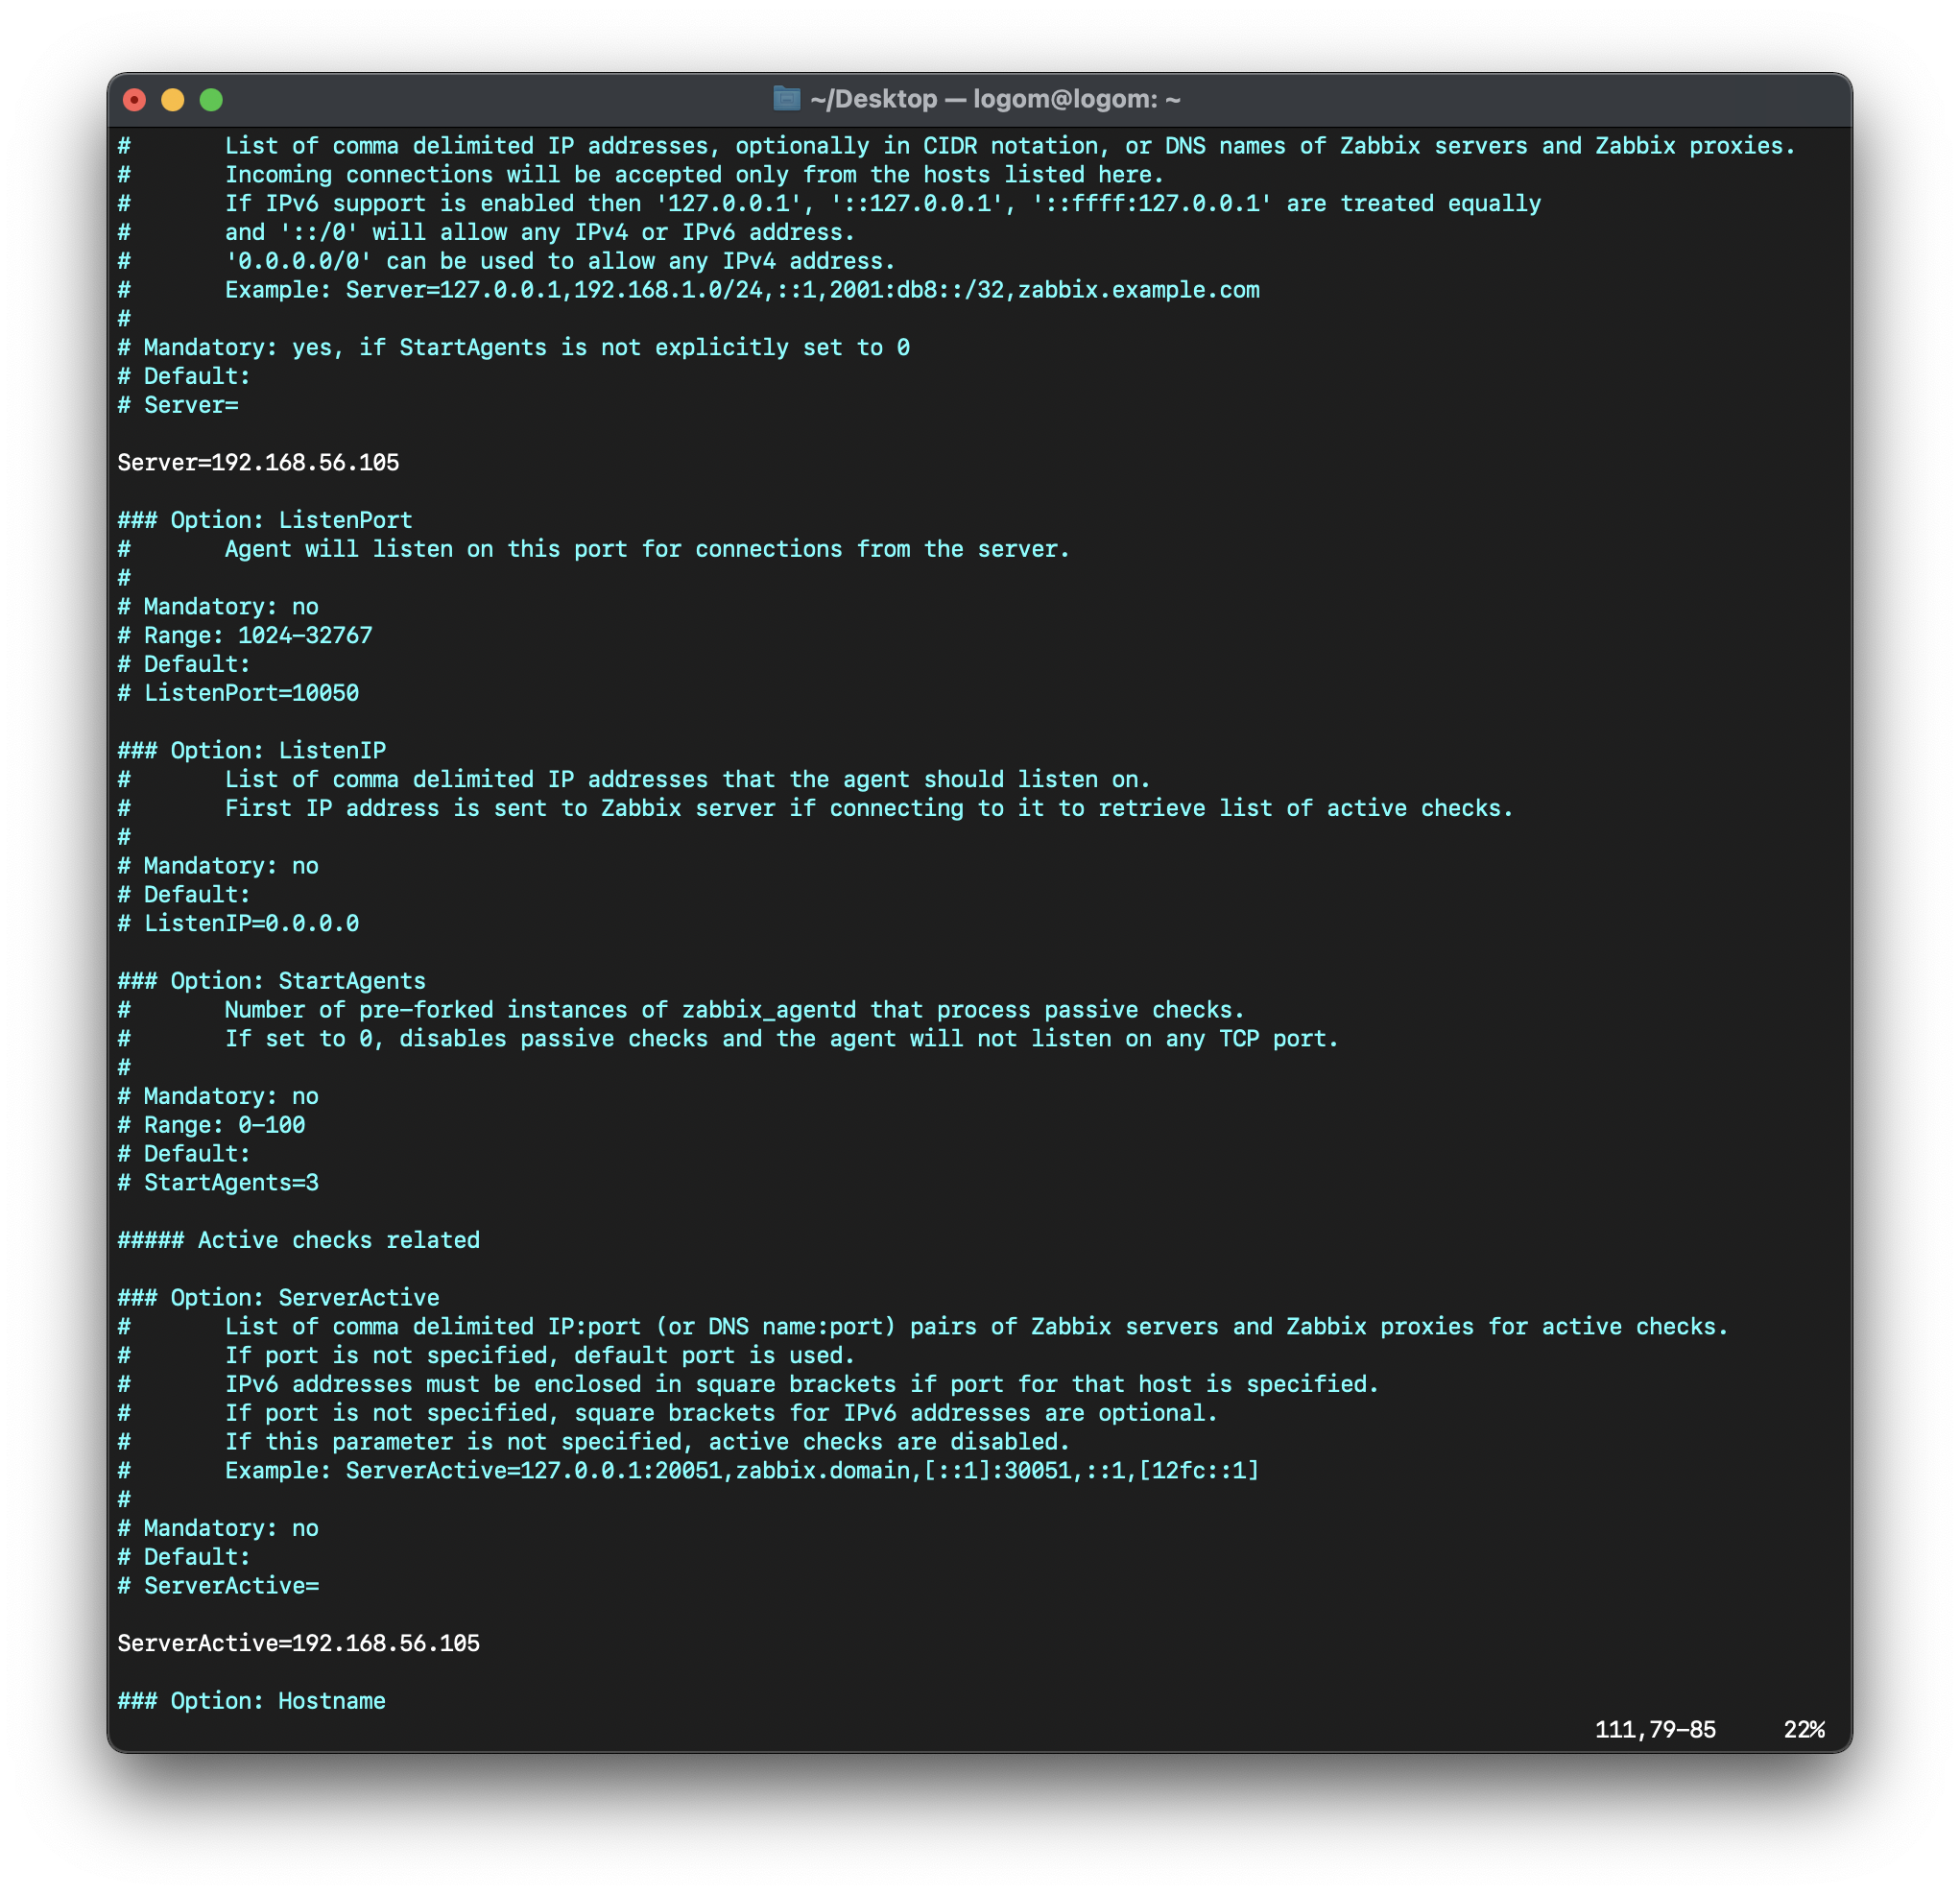
\includegraphics[scale=0.45]{images/ubuntu_servers.png}
            \caption{Configuración Server y ServerActive}
            \label{fig:ubuntu_servers}
        \end{figure}
        \begin{tcolorbox}[colback=black!10, halign=left]
            \$ sudo systemctl restart zabbix-agent
        \end{tcolorbox}

%%%%%%%%%%%%%%%%%%%%%%%%%%%%%%%%%%%%%%%%%% 
% Apartado para la instalación en CentOS %
%%%%%%%%%%%%%%%%%%%%%%%%%%%%%%%%%%%%%%%%%% 
\newpage
\subsection{Instalación de Zabbix en CentOS}
    \subsubsection{Descargar paquetes de Zabbix 5.0}
    Vamos a descargar los paquetes de Zabbix, para ello entramos en su web oficial, \href{https://www.zabbix.com/download}{Zabbix.com}, y 
    seleccionamos los siguientes parámetros ya que son los que se ajustan a nuestras necesidades.
    \begin{figure}[H]
        \centering
        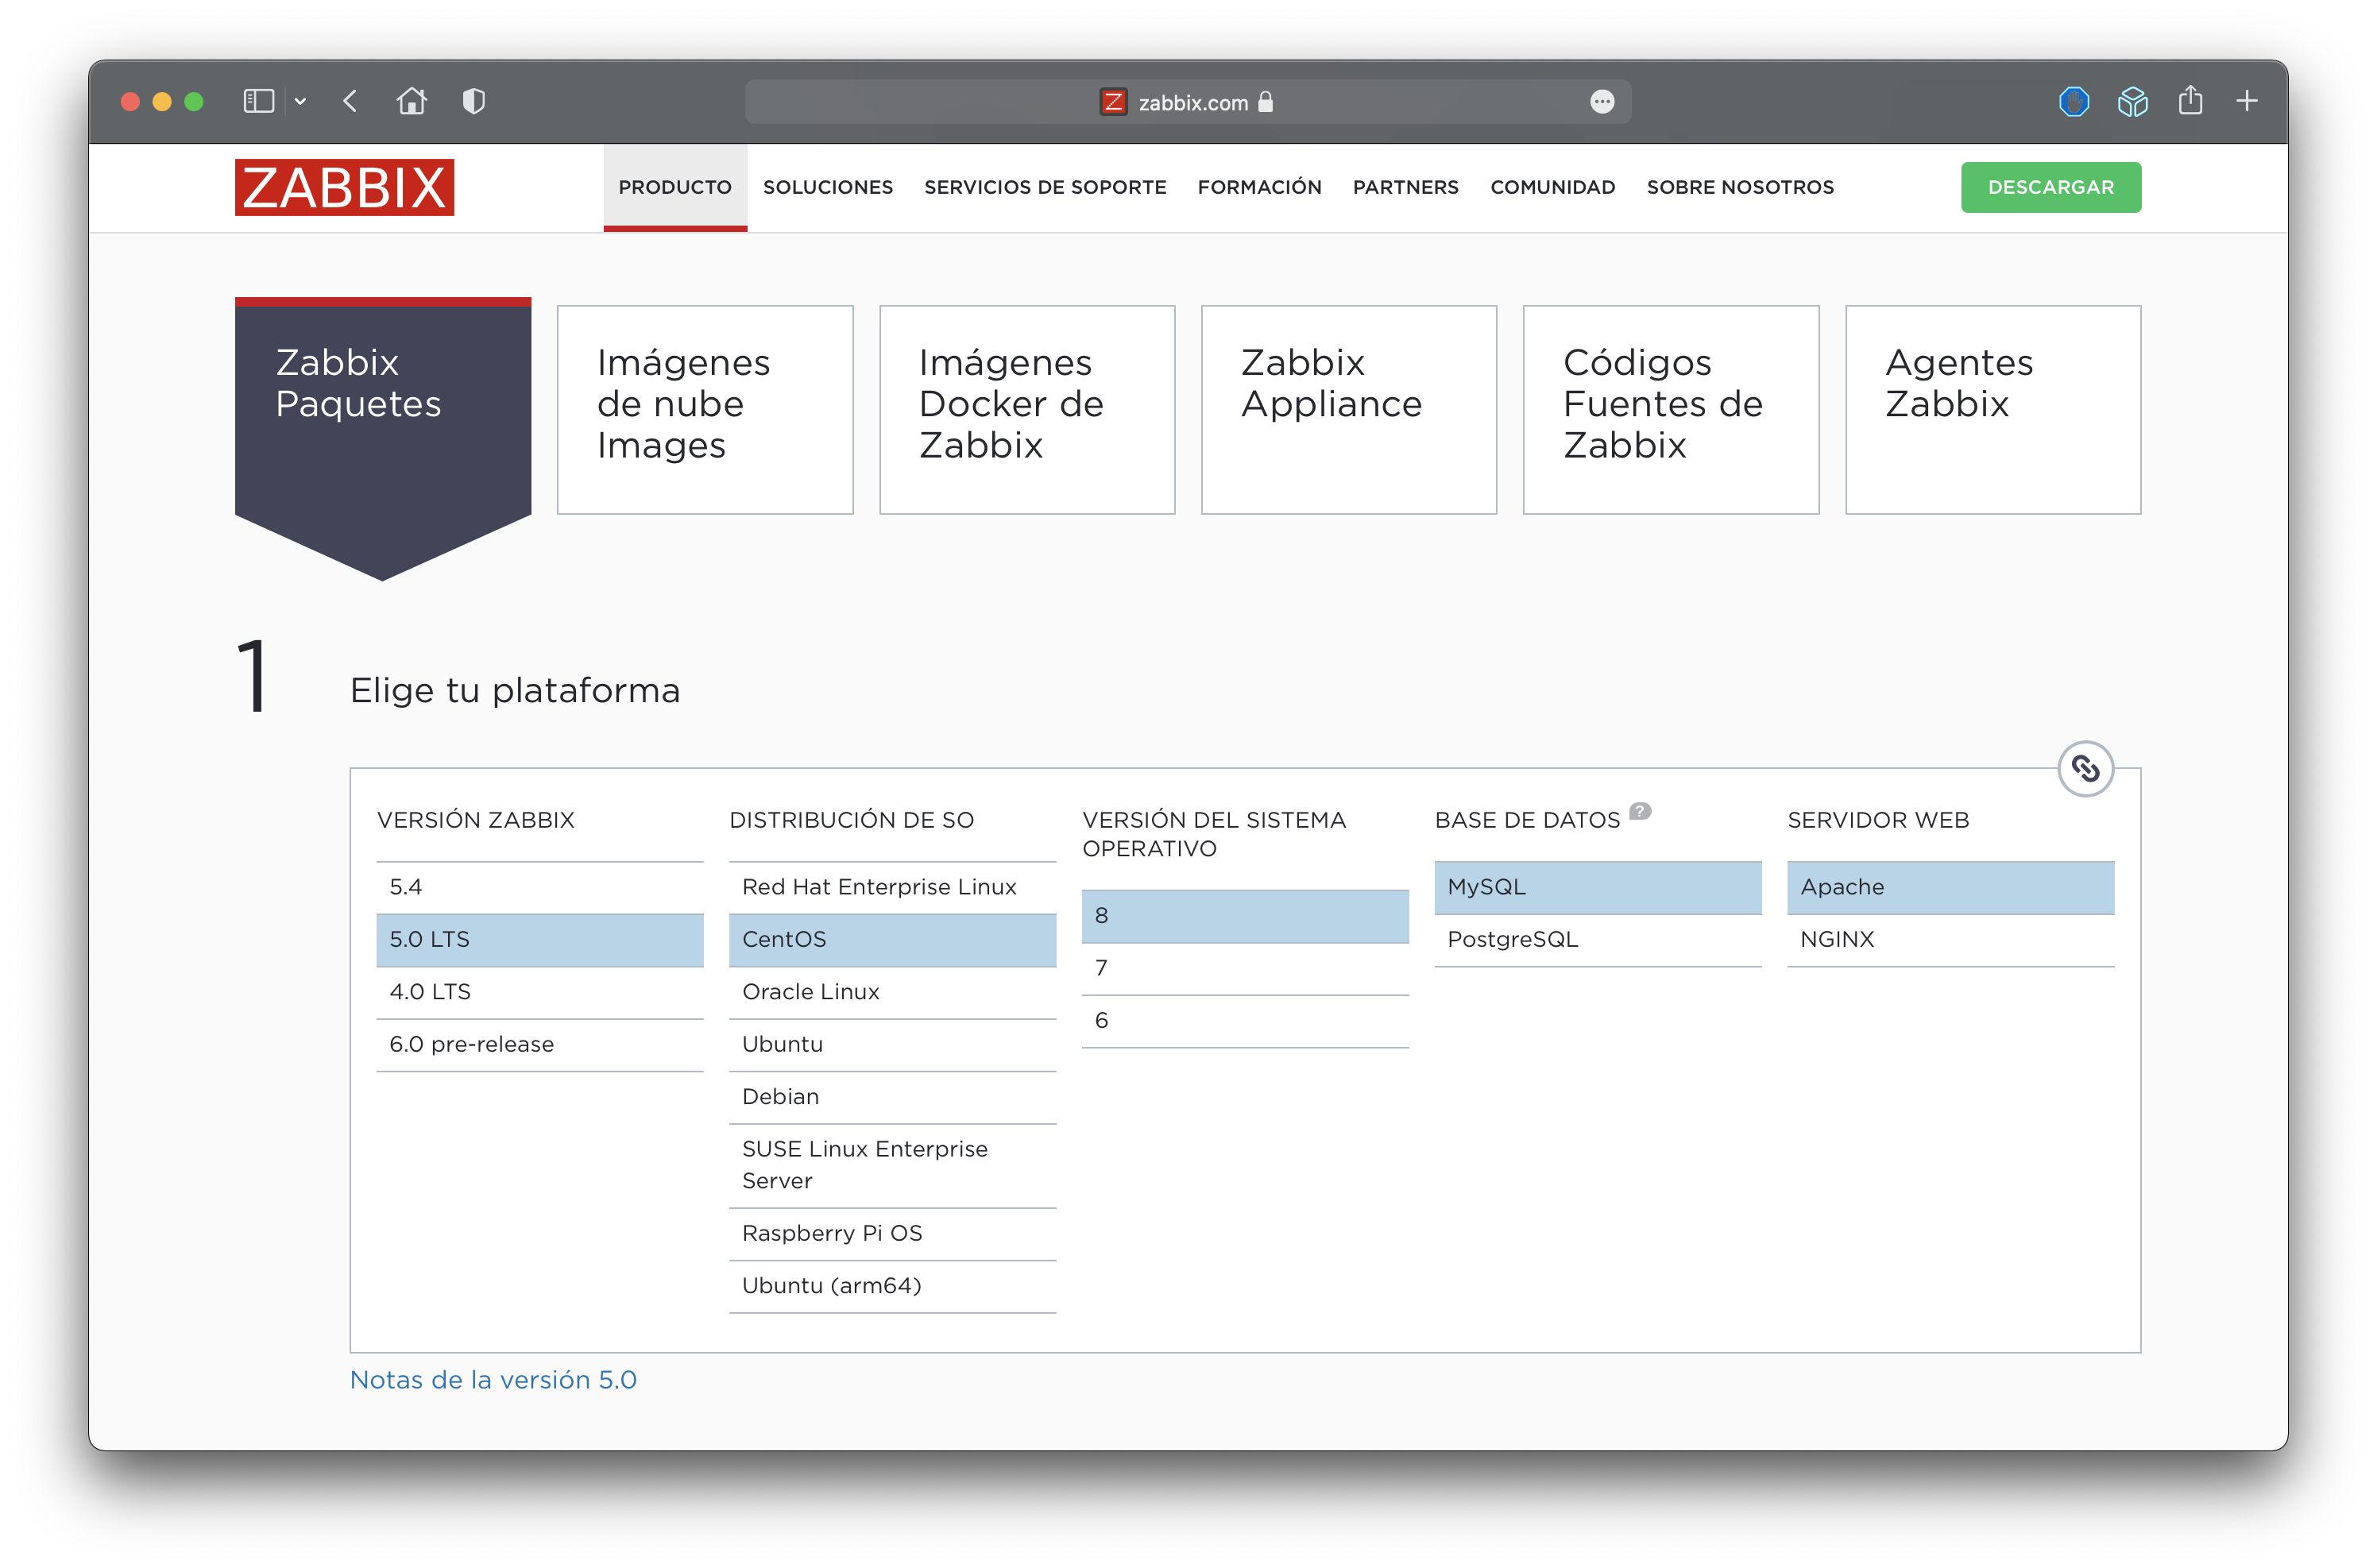
\includegraphics[scale=0.3]{images/zabbix_centOS.png}
        \caption{Descargar Zabbix desde paquetes}
        \label{fig:zabbix_centOS}
    \end{figure}

    Lo primero que debemos hacer es descargar los paquetes correspondientes a Zabbix 5.0 desde su repositorio oficial con el comando \textbf{\emph{wget}}. 
        \begin{tcolorbox}[colback=black!10, halign=left]
            \# sudo rpm -Uvh https://repo.zabbix.com/zabbix/5.0/rhel/8/x86\_64/zabbix-release-5.0-1.el8.noarch.rpm
        \end{tcolorbox}

    Una vez descargado, limpiamos el directorio.
        \begin{tcolorbox}[colback=black!10, halign=left]
            \# sudo dnf clean all
        \end{tcolorbox}

    Por último, instalamos el servidor, la interfaz y el agente de Zabbix.
        \begin{tcolorbox}[colback=black!10, halign=left]
            \# dnf install zabbix-server-mysql zabbix-web-mysql zabbix-apache-conf zabbix-agent
        \end{tcolorbox}

    \subsubsection{Habilitar los puertos de escucha}
    Activamos el puerto 10050 ya que es el puerto por defecto del agente de forma permanente con el siguiente comando: 
        \begin{tcolorbox}[colback=black!10, halign=left]
            \# sudo firewall-cmd --add-port=10050/tcp --permanent
        \end{tcolorbox}

    Una vez se ha habilitado, recargamos para que se active sin necesidad de reiniciar la máquina.
    \begin{tcolorbox}[colback=black!10, halign=left]
        \# sudo firewall-cmd --reload
    \end{tcolorbox}
    
    \subsubsection{Configurar el fichero de agente}
    Editamos el fichero que se encuentra en \textbf{/etc/zabbix/zabbix\_agentd.conf} y cambiamos los parámetos \textbf{\emph{server}} y \textbf{\emph{serverActive}}
    con la IP del servidor que queremos que monitorice este sistema, en nuestro caso \textbf{192.168.56.105}. 

    \begin{figure}[H]
        \centering
        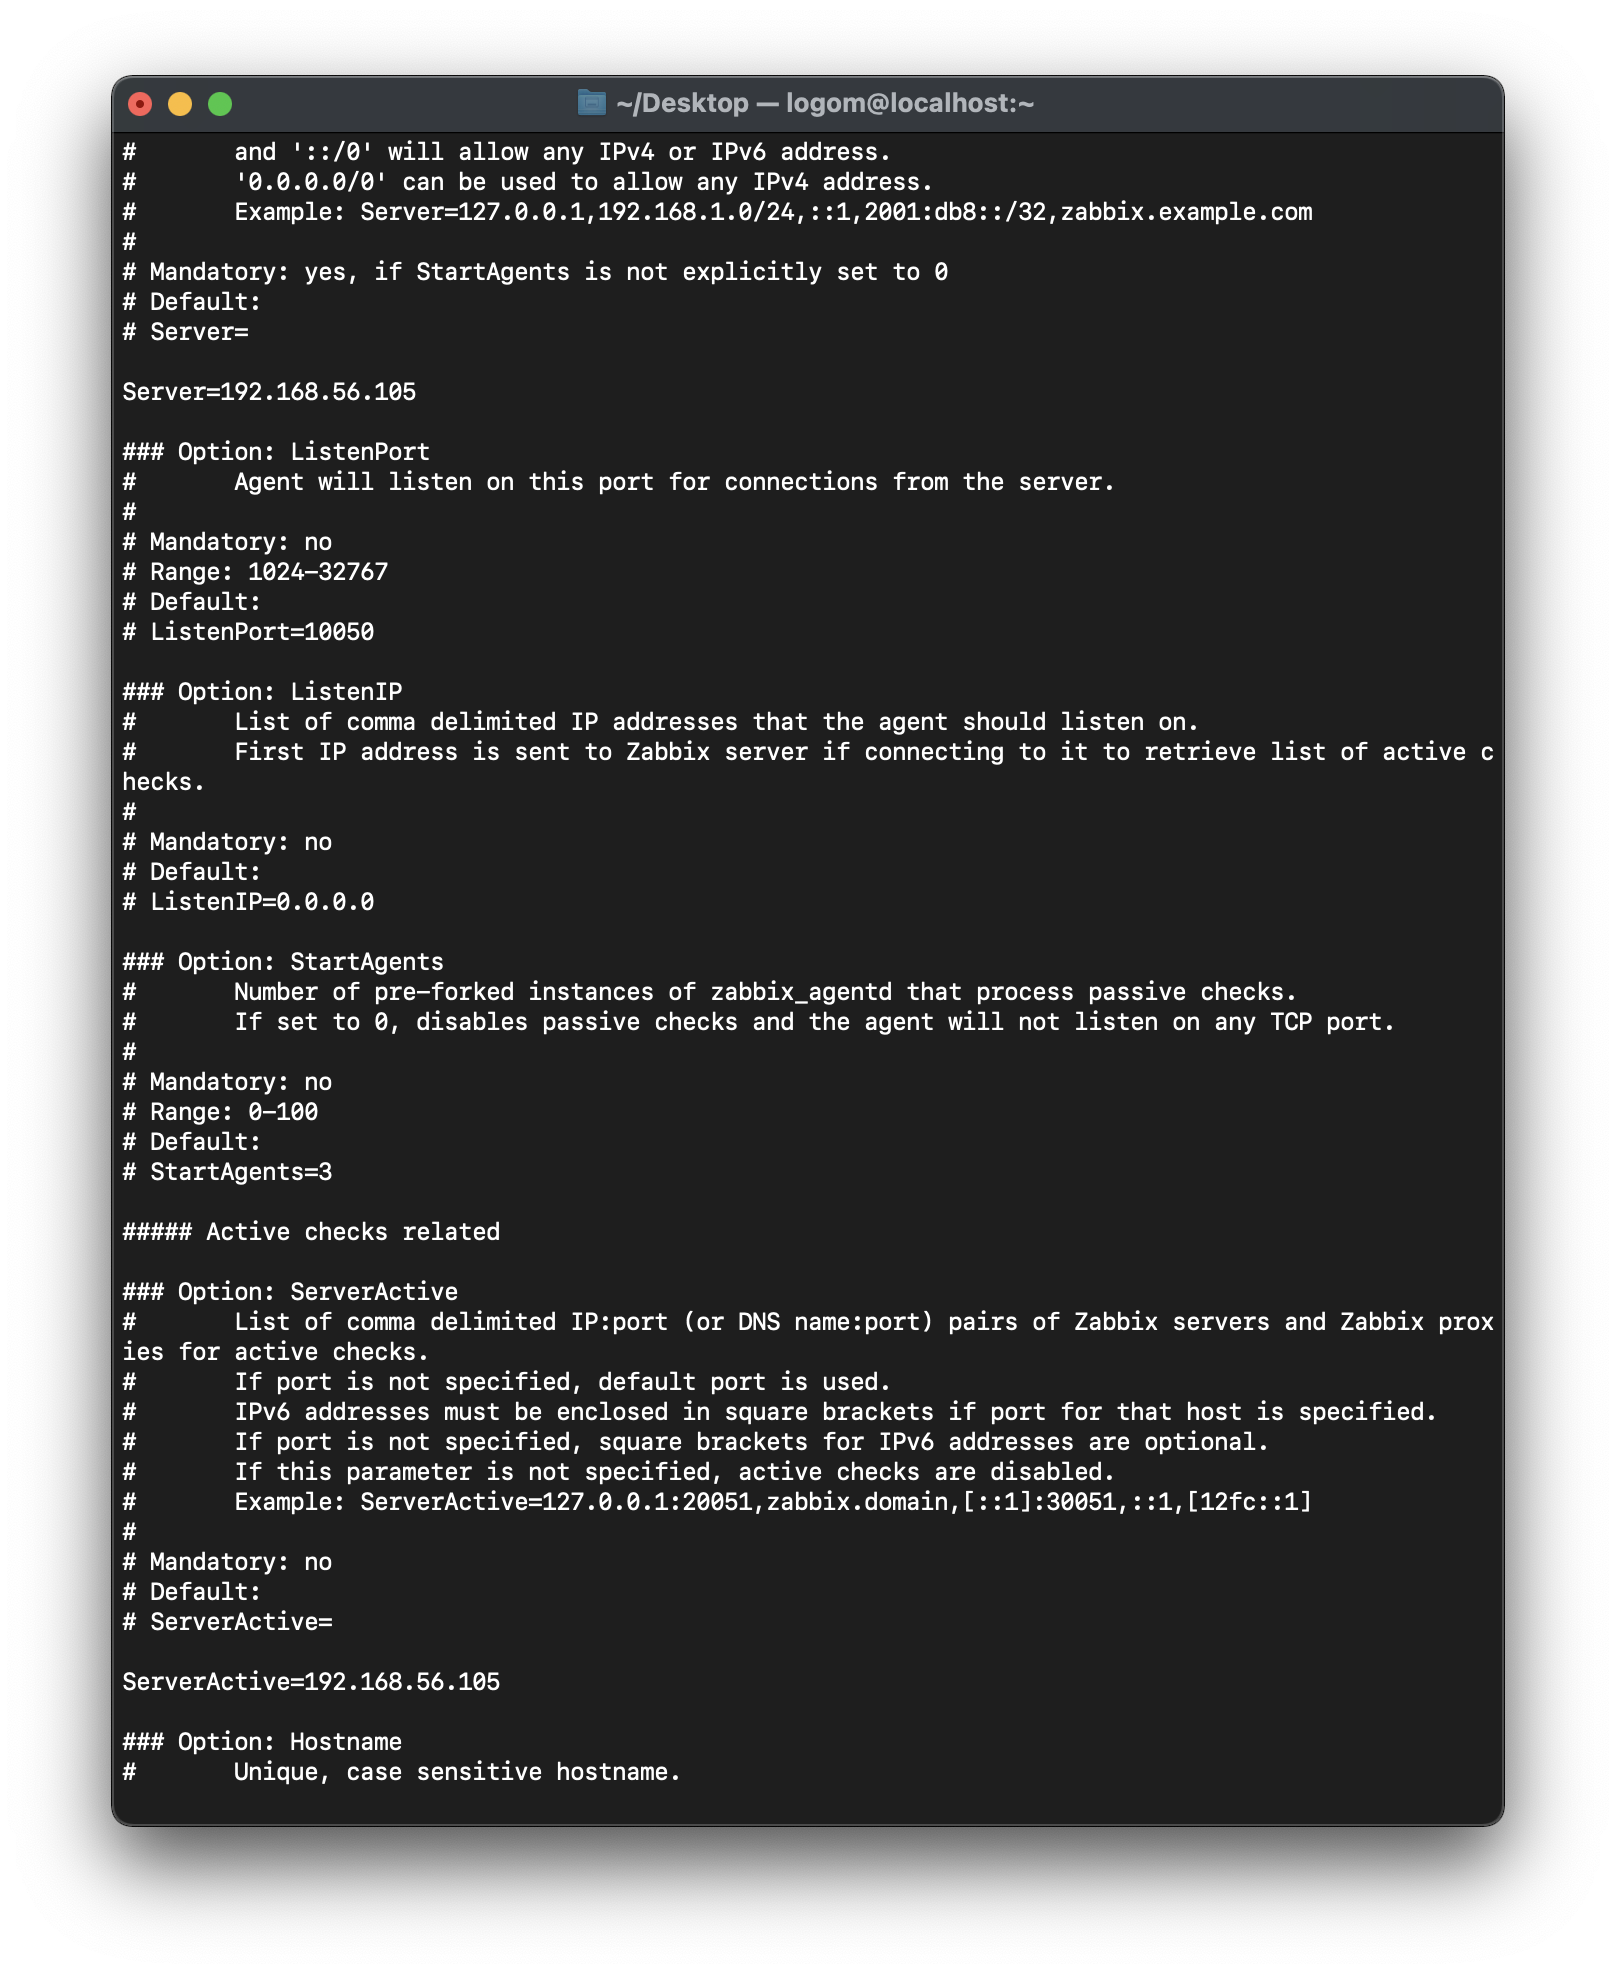
\includegraphics[scale=0.4]{images/centos_servers.png}
        \caption{Configuración Server y ServerActive}
        \label{fig:centos_servers}
    \end{figure}    

    \subsubsection{Configurar los servicios}
    Reiniciamos los servicios \textbf{\emph{zabbix-server}}, \textbf{\emph{zabbix-agent}} y \textbf{\emph{apache2}} para que se actualicen los cambios realizados.
        \begin{tcolorbox}[colback=black!10, halign=left]
            \# sudo systemctl restart zabbix-server zabbix-agent httpd php-fpm
        \end{tcolorbox}

    Habilitamos los servicios anteriores para que se enciendan cuando arranque el sistema.
        \begin{tcolorbox}[colback=black!10, halign=left]
            \# sudo systemctl enable zabbix-server zabbix-agent httpd php-fpm
        \end{tcolorbox}

%%%%%%%%%%%%%%%%%%%%%%%%%%%%%%%%%%%%%%%%%% 
% Apartado para la instalación en CentOS %
%%%%%%%%%%%%%%%%%%%%%%%%%%%%%%%%%%%%%%%%%% 
\subsection{Instalación del Front-End}
    \subsubsection{Página de bienvenida de Zabbix}
    Desde un navegador ingresamos en la dirección \textbf{192.168.56.105/zabbix}. Nos aparecerá una web de bienvenida con la varsión de Zabbix que estamos utilizando. 
    Pulsamos al botón \textbf{\emph{"Next Step"}} para continuar.
    \begin{figure}[H]
        \centering
        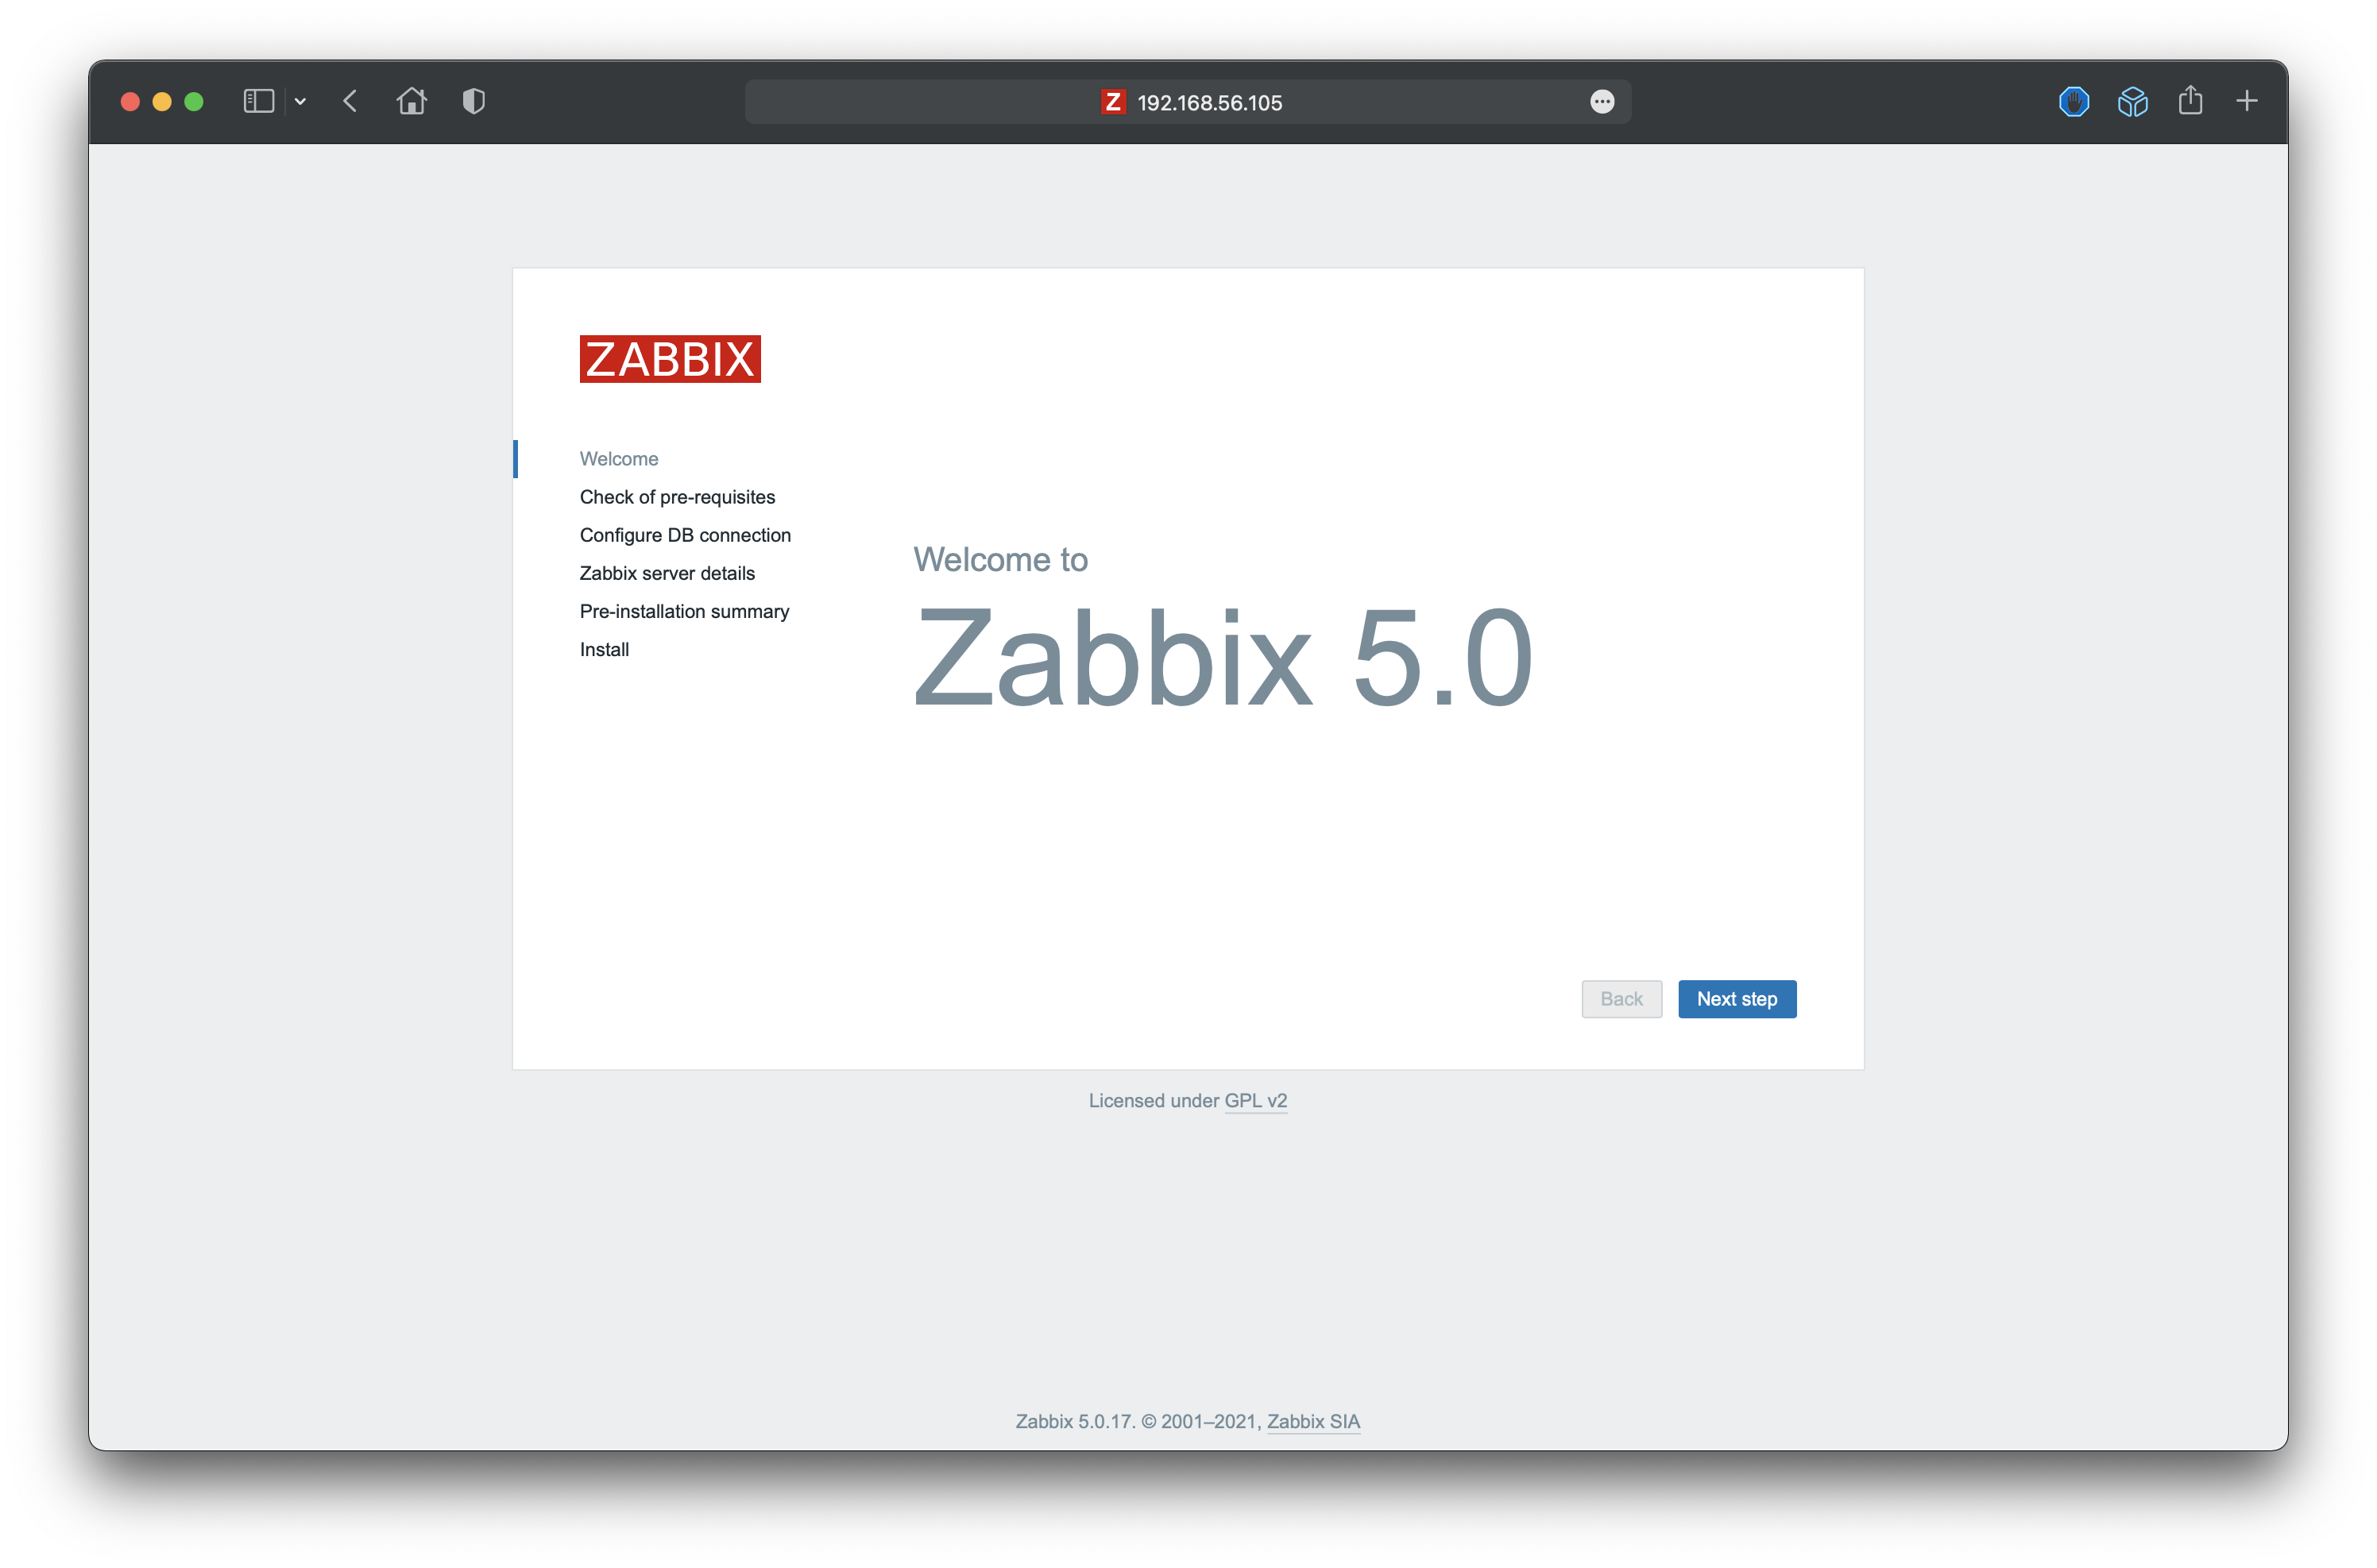
\includegraphics[scale=0.25]{images/zabbix_installation_1.png}
        \caption{Página de bienvenida de Zabbix}
        \label{fig:zabbix_installation_1}
    \end{figure}

    \subsubsection{Requisitos previos de Zabbix}
    En esta sección Zabbix nos muestra una lista de requisitos previos que deben de cumplirse para que todo funcione correctamente, si hubiera algún requisito que no se esté 
    cumpliendo habría que corregirlo. Una vez que verificamos que todos los requisitos se cumplen avanzamos al siguiente apartado pulsando en \textbf{\emph{"Next Step"}}.
    \begin{figure}[H]
        \centering
        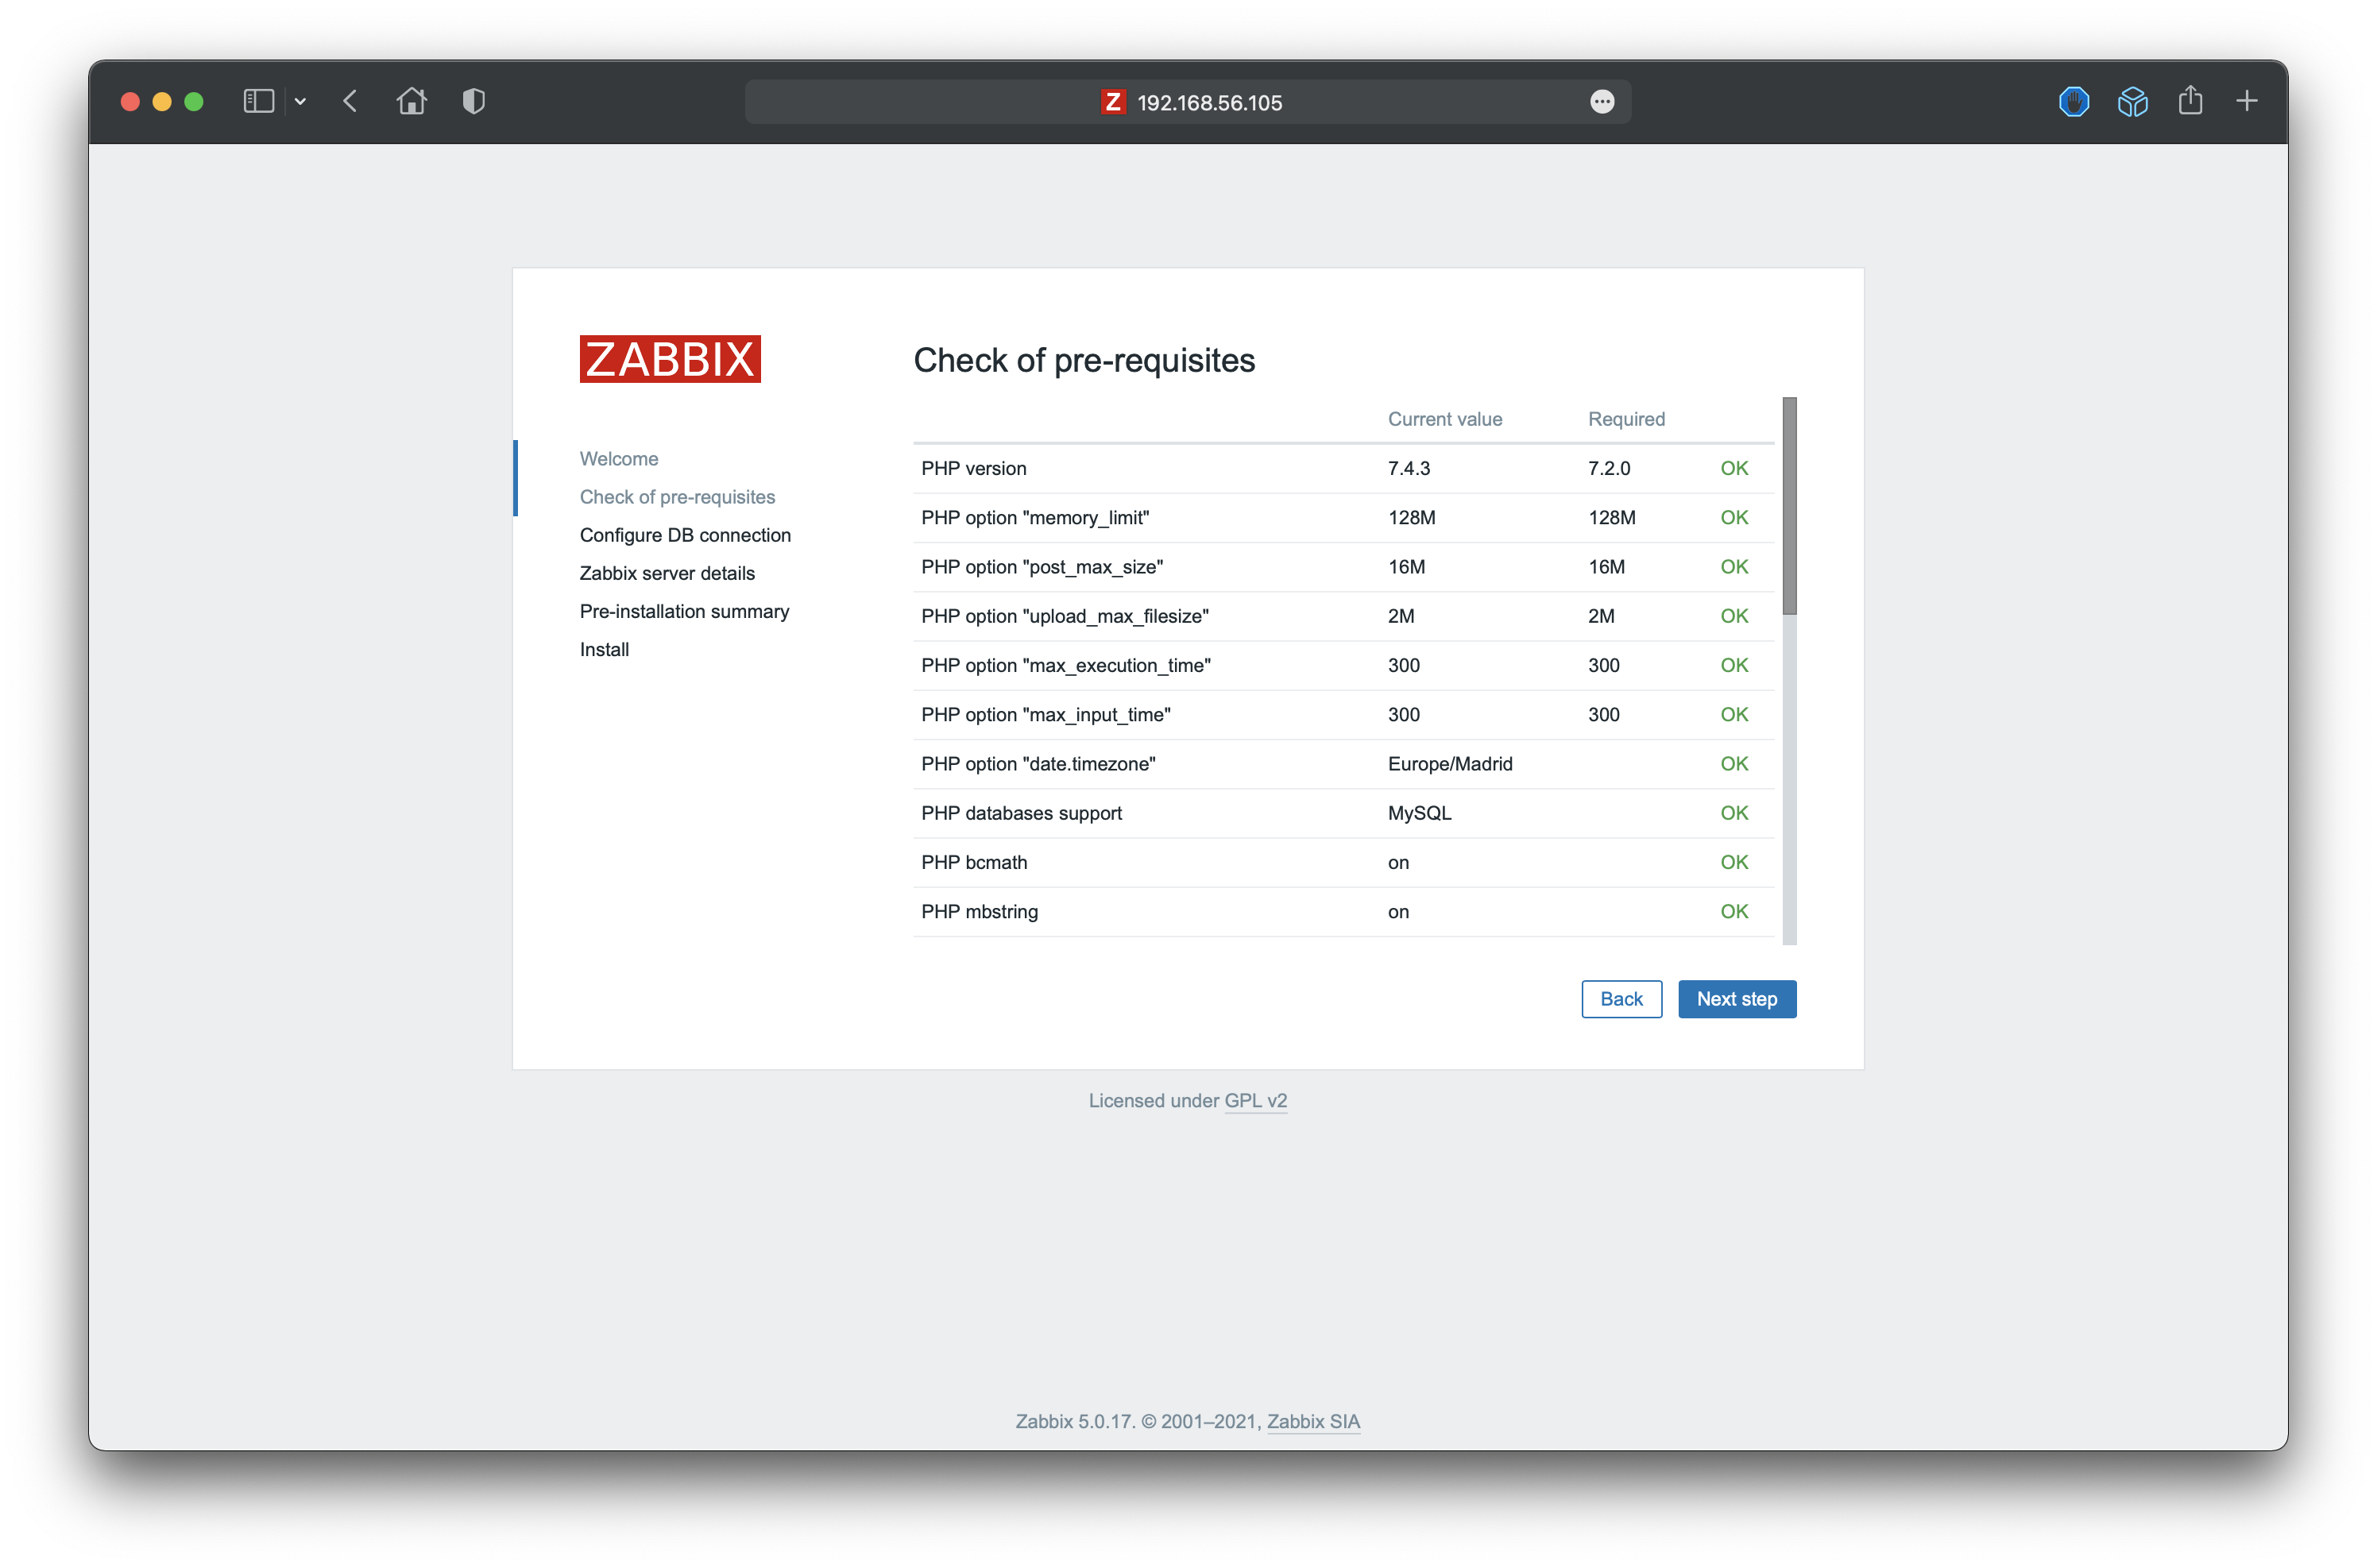
\includegraphics[scale=0.25]{images/zabbix_installation_2.png}
        \caption{Requisitos previos de Zabbix}
        \label{fig:zabbix_installation_2}
    \end{figure}

    \subsubsection{Conexión con la base de datos}
    Configuramos la conexión con la base de datos MySQL, escribimos \textbf{\emph{ISE}} como contraseña.
    \begin{figure}[H]
        \centering
        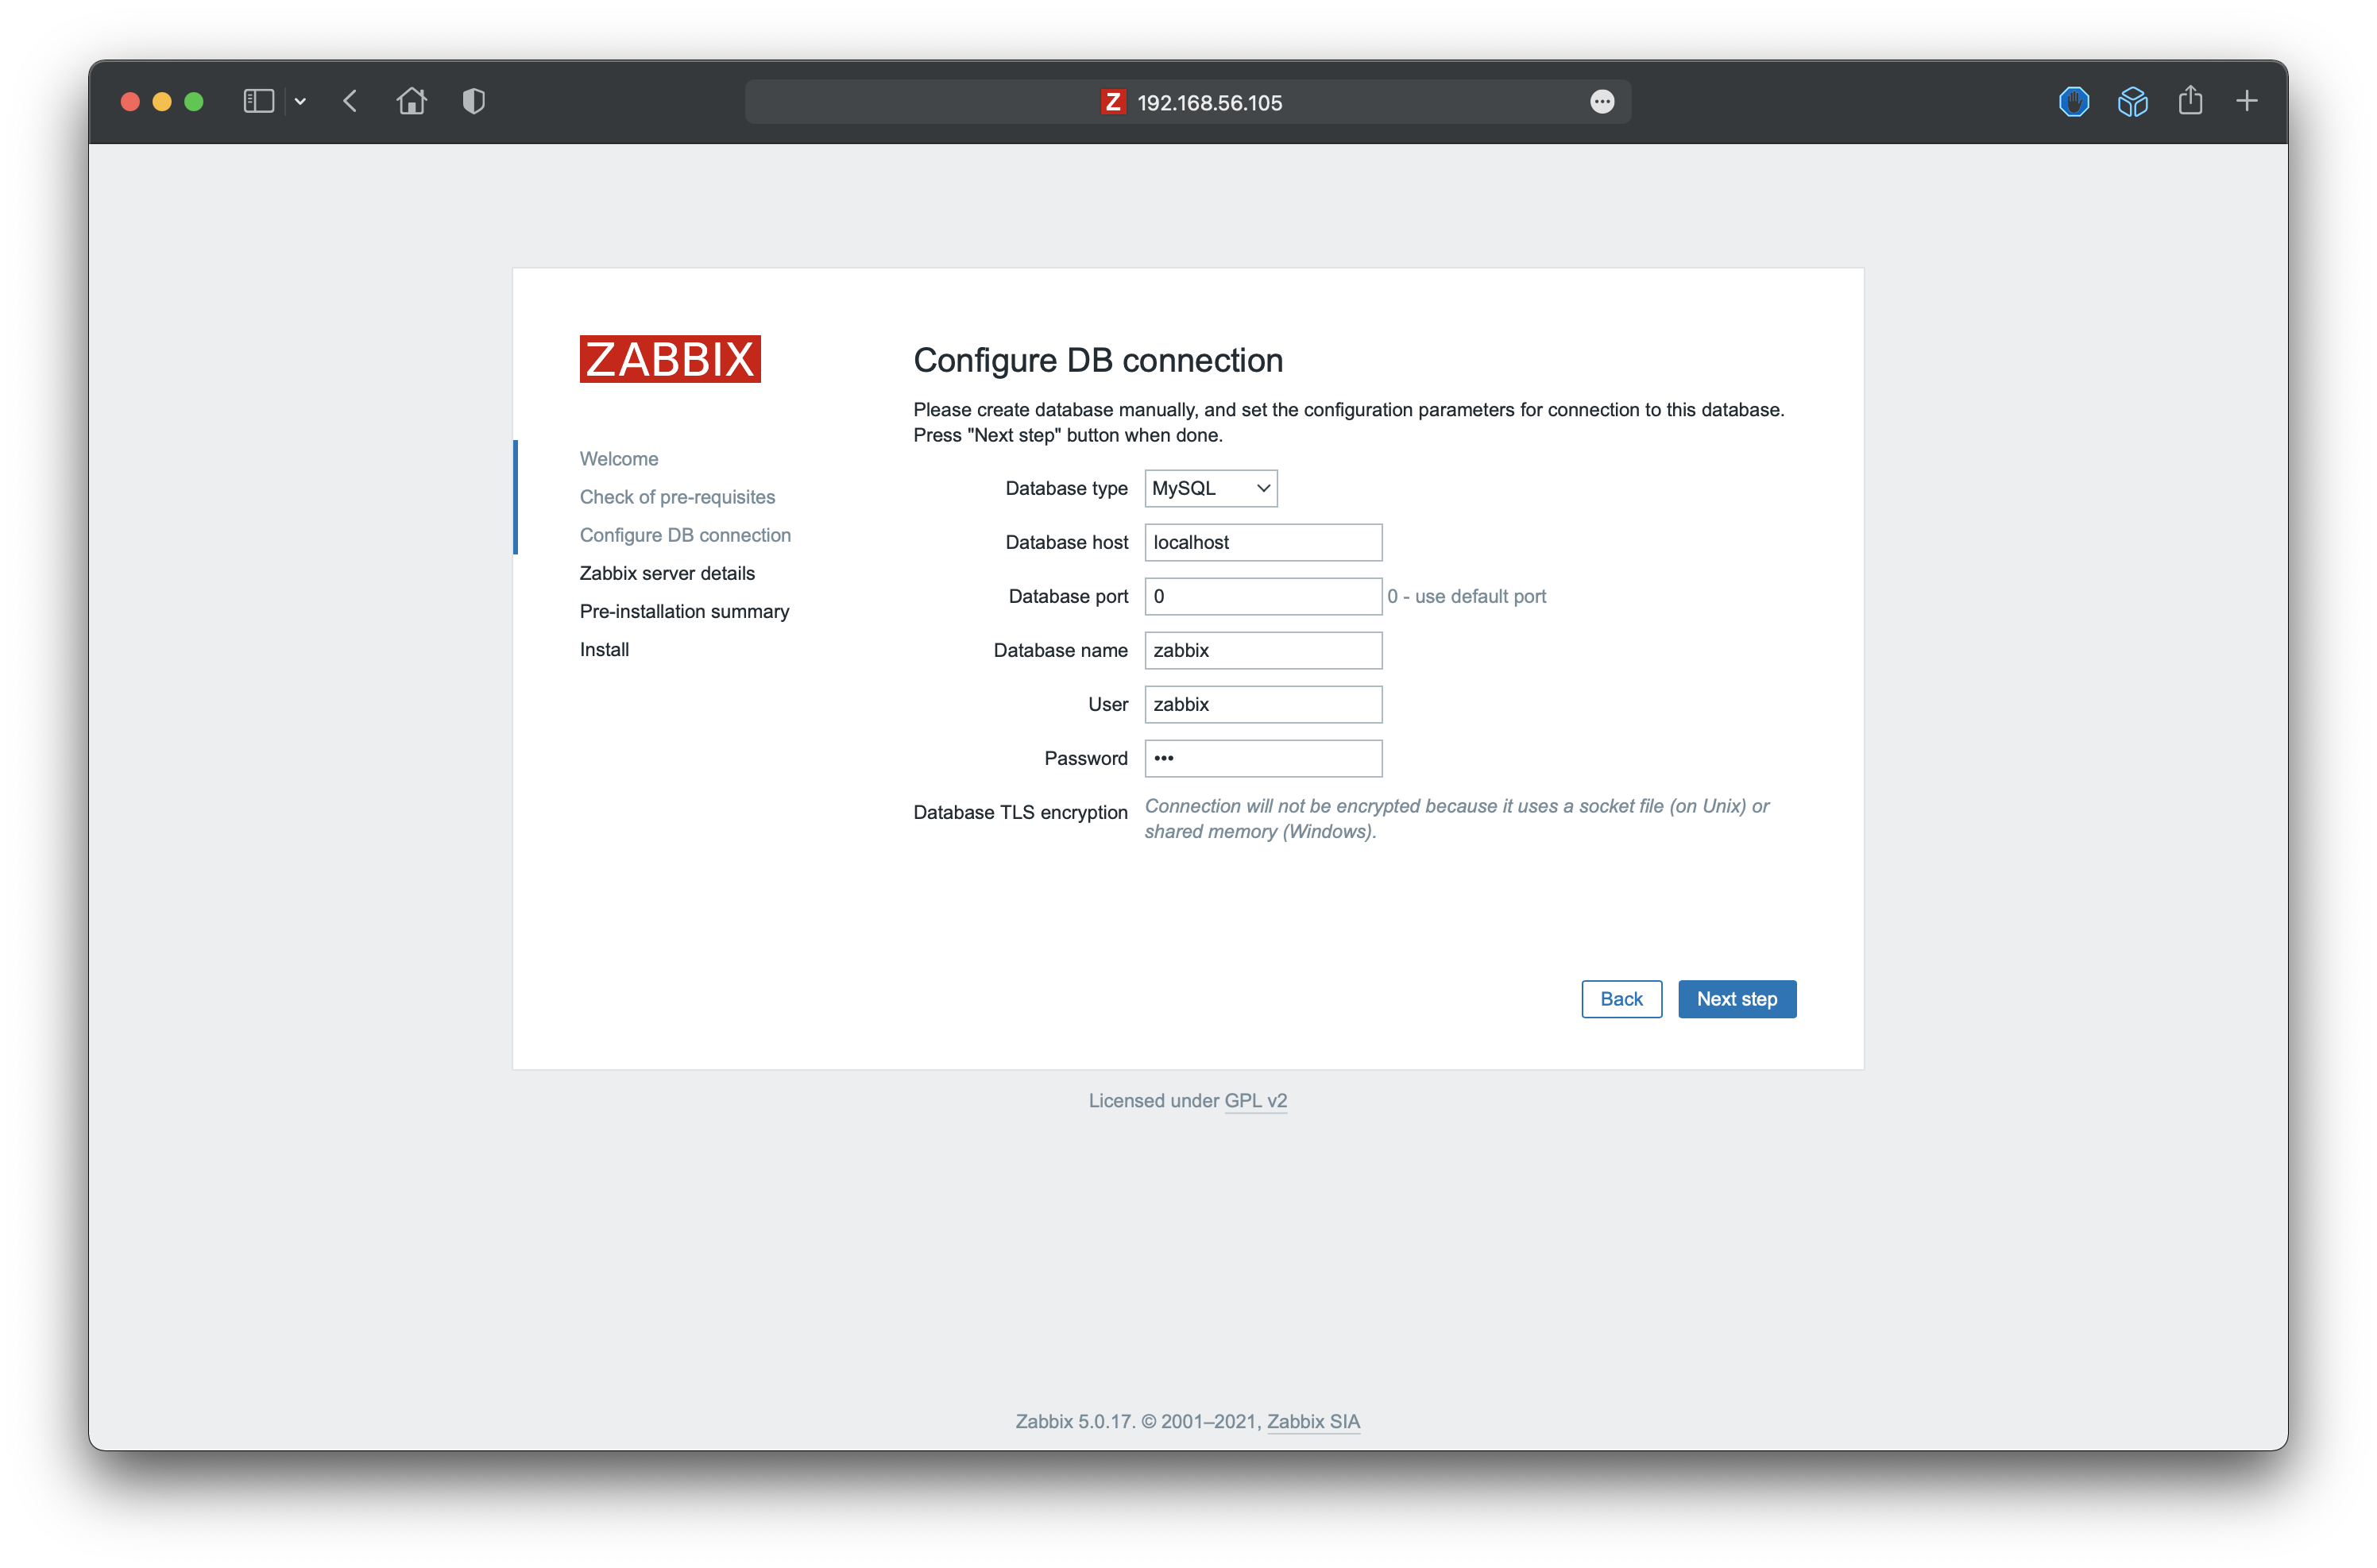
\includegraphics[scale=0.25]{images/zabbix_installation_3.png}
        \caption{Conexión con la base de datos}
        \label{fig:zabbix_installation_3}
    \end{figure}

    \subsubsection{Detalles del servidor}
    Ingresamos el nombre del host y el puerto que vamos a utilizar.
    \begin{figure}[H]
        \centering
        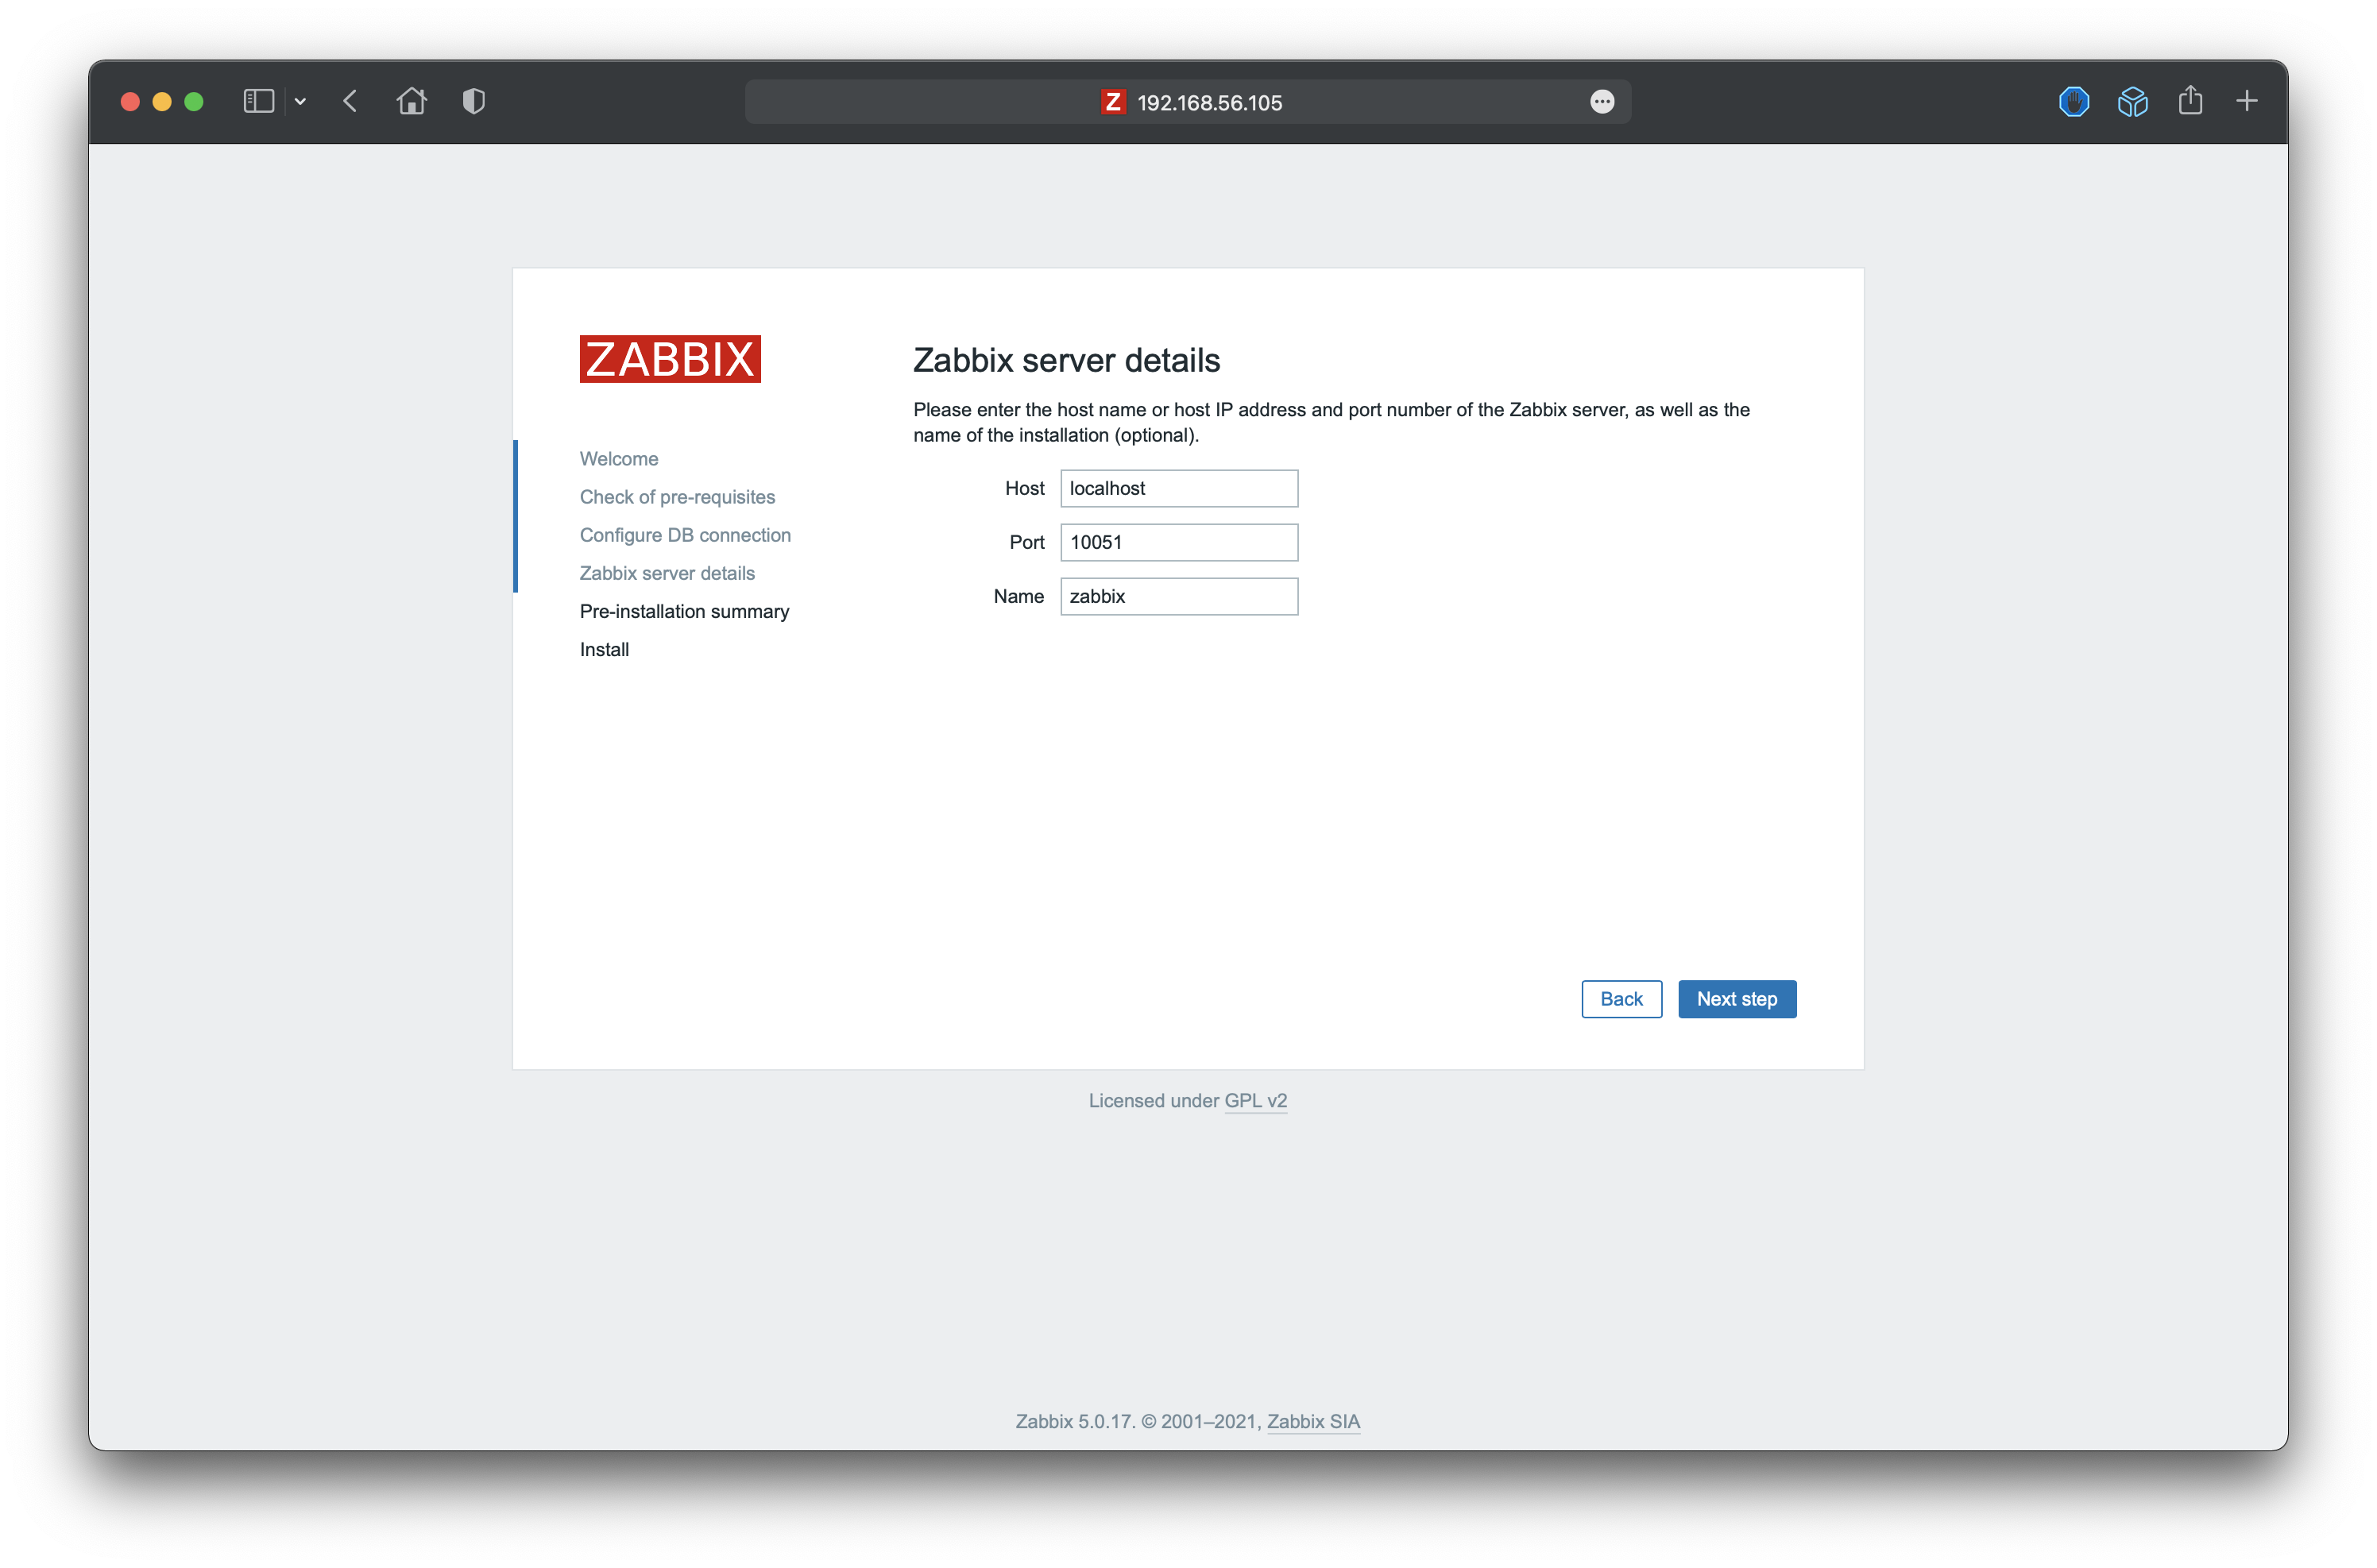
\includegraphics[scale=0.25]{images/zabbix_installation_4.png}
        \caption{Detalles del servidor}
        \label{fig:zabbix_installation_4}
    \end{figure} 

    \subsubsection{Instalación del Front-End}
    Comprobamos que todo está bien antes de instalar ya que no se podrá cambiar ningún parámetro.
    \begin{figure}[H]
        \centering
        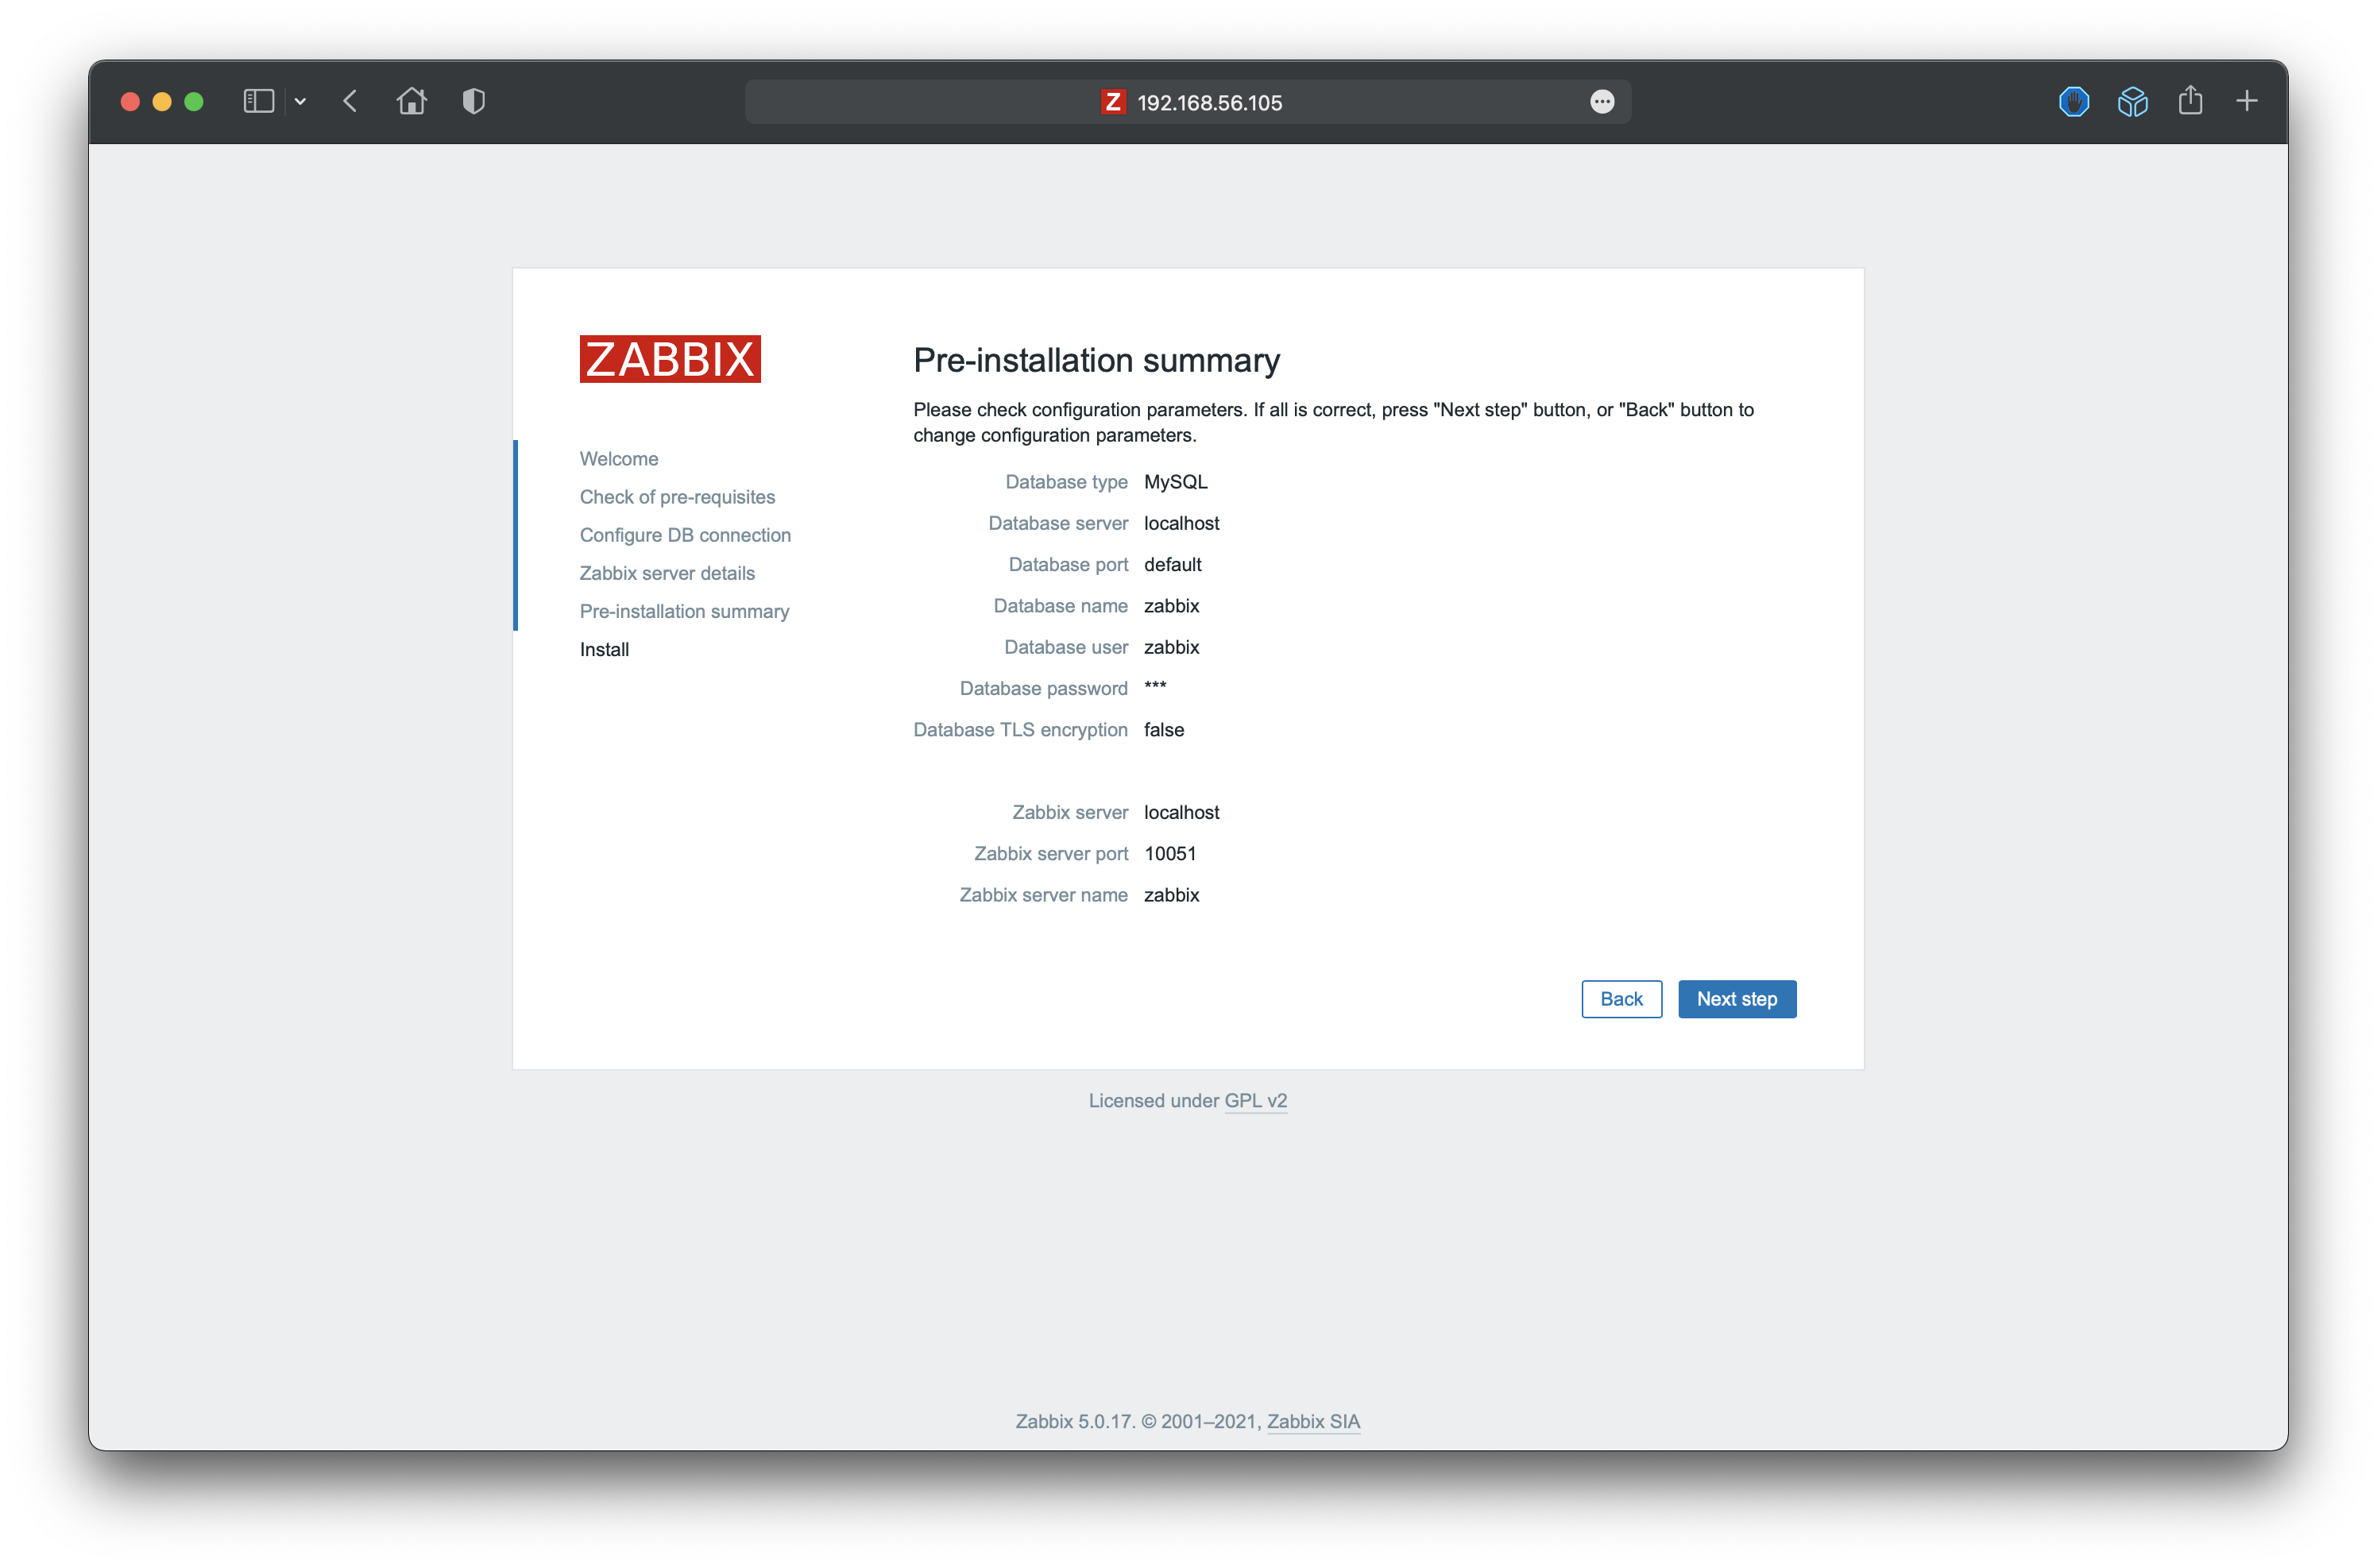
\includegraphics[scale=0.25]{images/zabbix_installation_5.png}
        \caption{Instalación del Front-End}
        \label{fig:zabbix_installation_5}
    \end{figure}

%%%%%%%%%%%%%%%%%%%%%%%%%%%%%%%%%%%%%%%%%%%%%%%%%%
% Apartado para la monitorizacación de los hosts %
%%%%%%%%%%%%%%%%%%%%%%%%%%%%%%%%%%%%%%%%%%%%%%%%%%
\newpage
\section{Configuración para la monitorización de los hosts}
\subsection{Web de gestión de Zabbix}
Desde un navegador a la web de gestión de monitorización y accedemos como usuario \textbf{\emph{Admin}} con contraseña \textbf{\emph{zabbix}} para acceder como administrador
para poder gestionar la monitorización.
    \begin{figure}[H]
        \centering
        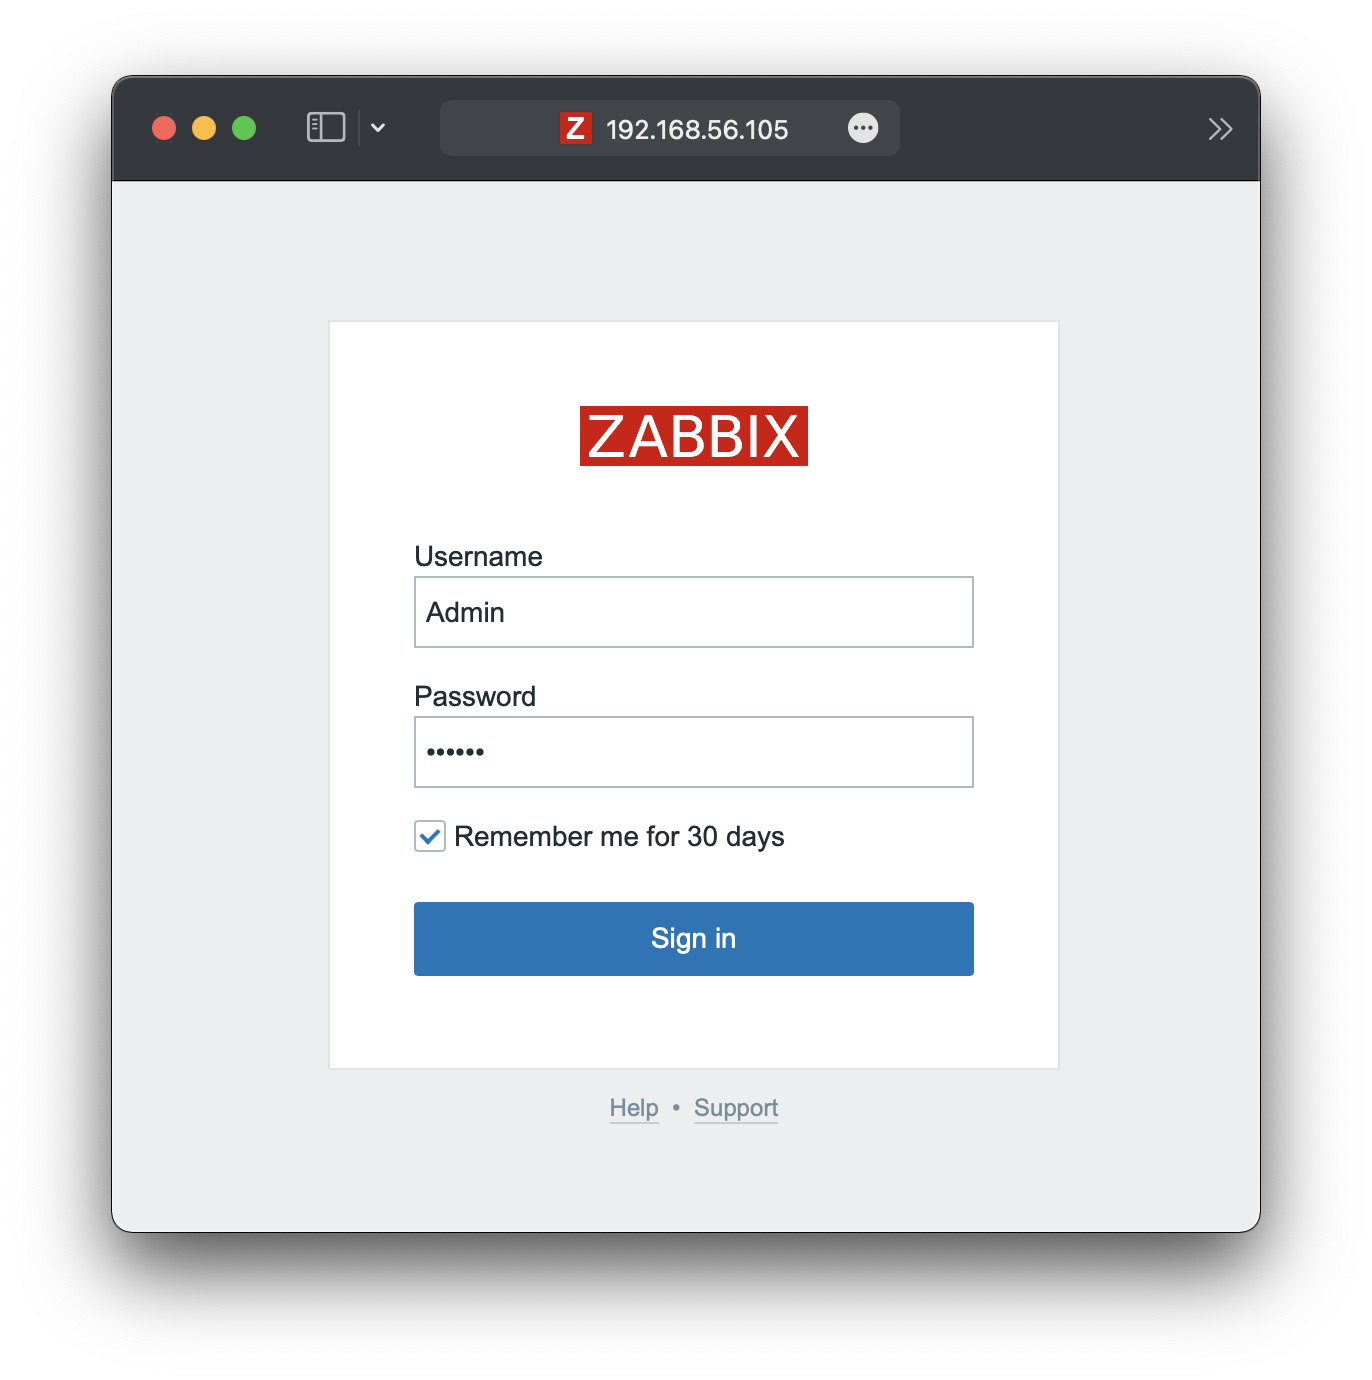
\includegraphics[scale=0.35]{images/zabbix_login.png}
        \caption{Iniciar Sesión en Zabbix}
        \label{fig:zabbix_login}
    \end{figure}

Una vez dentro, accedemos al apartado de hosts (desplegable ubicado a la izquierda) en configuración y pulsamos sobre \textbf{\emph{Create host}}.
    \begin{figure}[H]
        \centering
        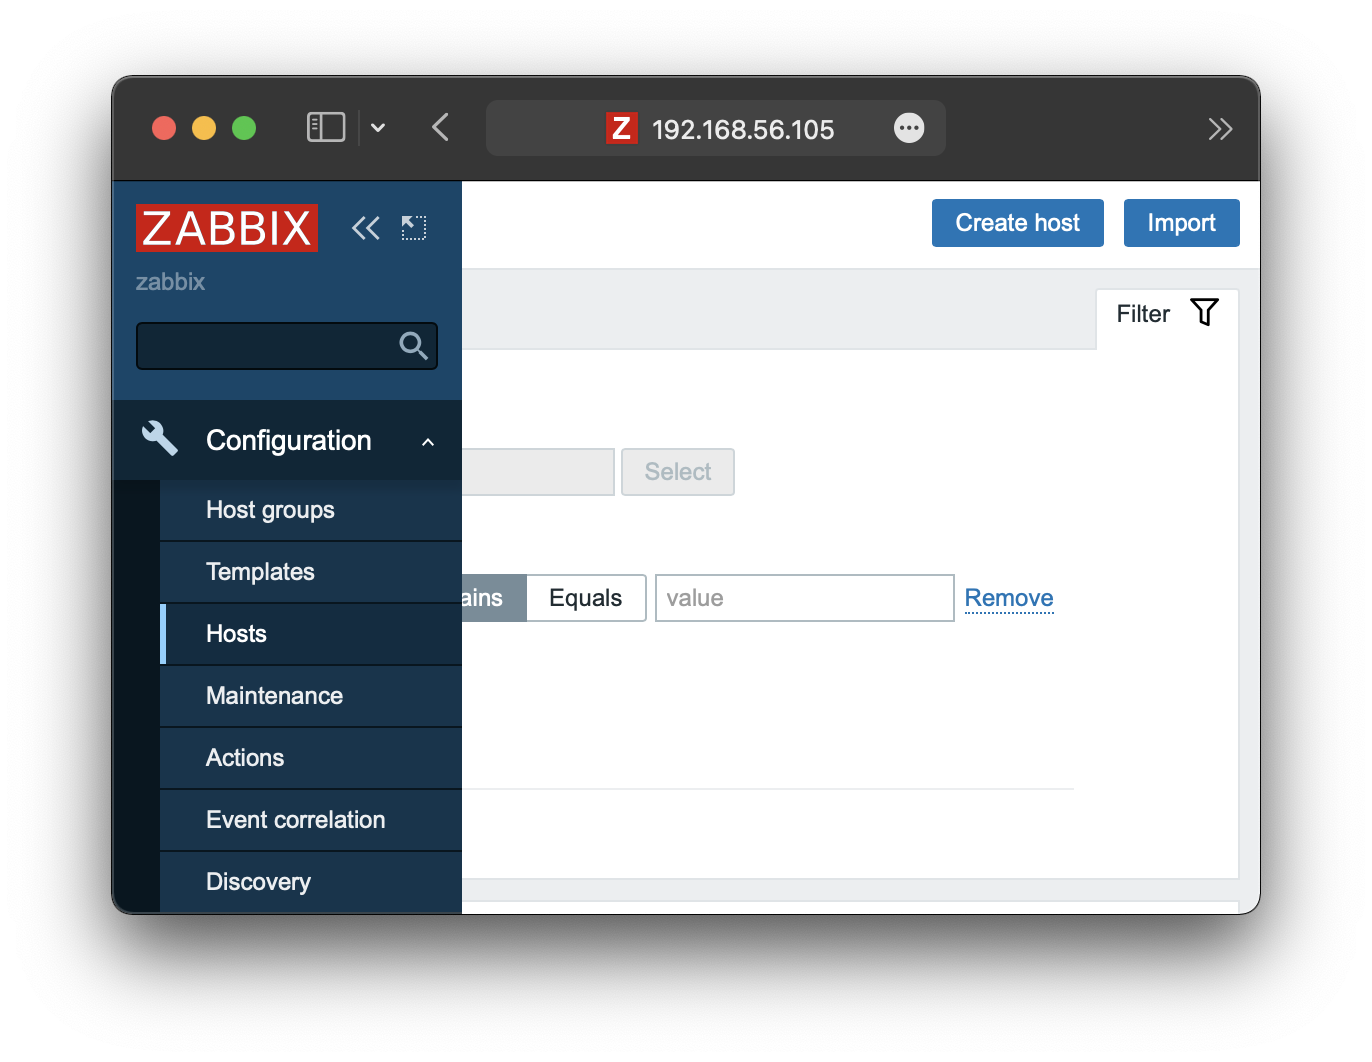
\includegraphics[scale=0.4]{images/zabbix_hosts.png}
        \caption{Crear hosts}
        \label{fig:zabbix_hosts}
    \end{figure}

\subsection{Configuración del host Ubuntu Server}
\subsubsection{Apartado Host}
En este apartado definiremos el nombre con el que identificaremos la máquina con Ubuntu Server, los grupos a los que pertenece, la IP de la máquina y el puerto de escucha.
Rellenamos los campos anteriores de la siguiente forma:
    \begin{itemize}
        \item \textbf{Host name:} Ubuntu Server
        \item \textbf{Groups:} Linux Servers | Virtual machines | Zabbix servers
        \item \textbf{IP address:} 192.168.56.105
        \item \textbf{Port:} 10050
    \end{itemize}
    \begin{figure}[H]
        \centering
        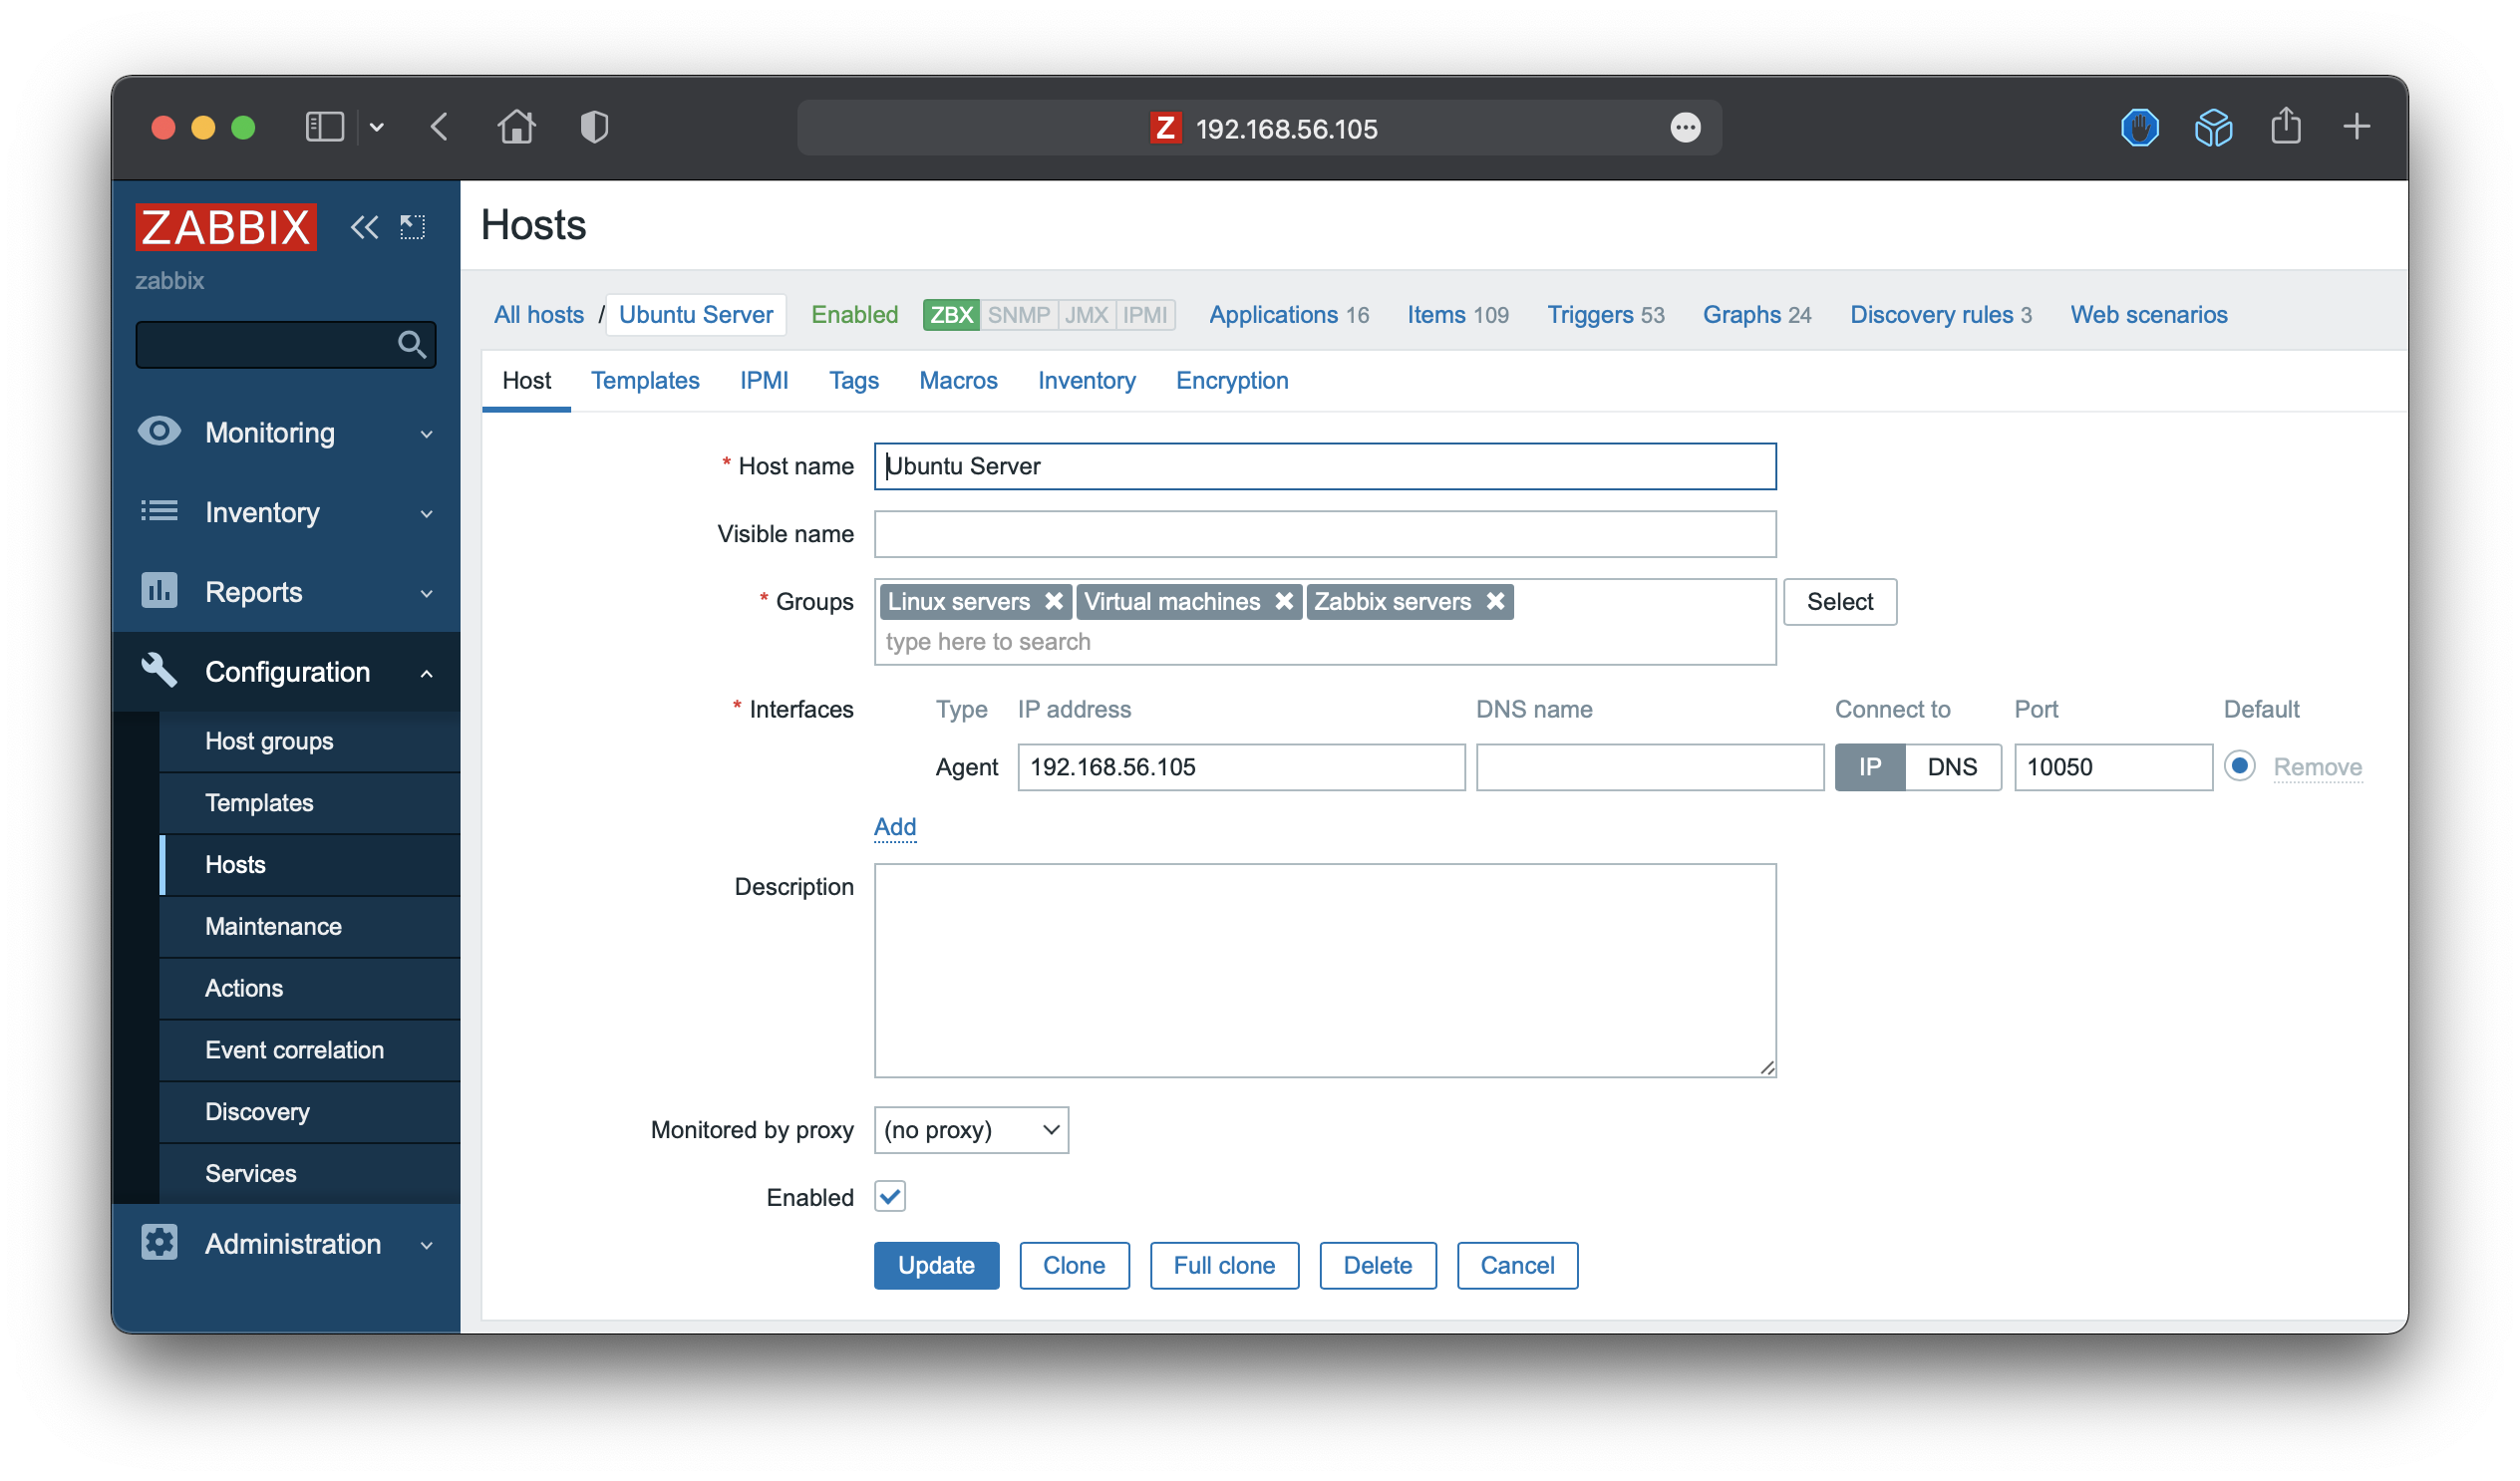
\includegraphics[scale=0.35]{images/ubuntu_server_conf.png}
        \caption{Configuración apartado host de Ubuntu Server}
        \label{fig:ubuntu_server_conf}
    \end{figure}
Una vez hemos rellenado los campos descritos anteriormente pulsamos el botón \textbf{\emph{Update}} para que se actualicen los campos.

\subsubsection{Apartado Templates}
En el apartado templates añadimos los templates necesarios de forma que tenga enlazados los siguientes templates:
    \begin{itemize}
        \item \textbf{Template App Apache by HTTP:} para monitorizar el servicio HTTP
        \item \textbf{Template App SSH Service:} para monitorizar el servicio SSH
        \item \textbf{Template App Zabbix Server:} indicamos el servidor
        \item \textbf{Template OS Linux by Zabbix agent:} indicamos el agente
    \end{itemize}
    \begin{figure}[H]
        \centering
        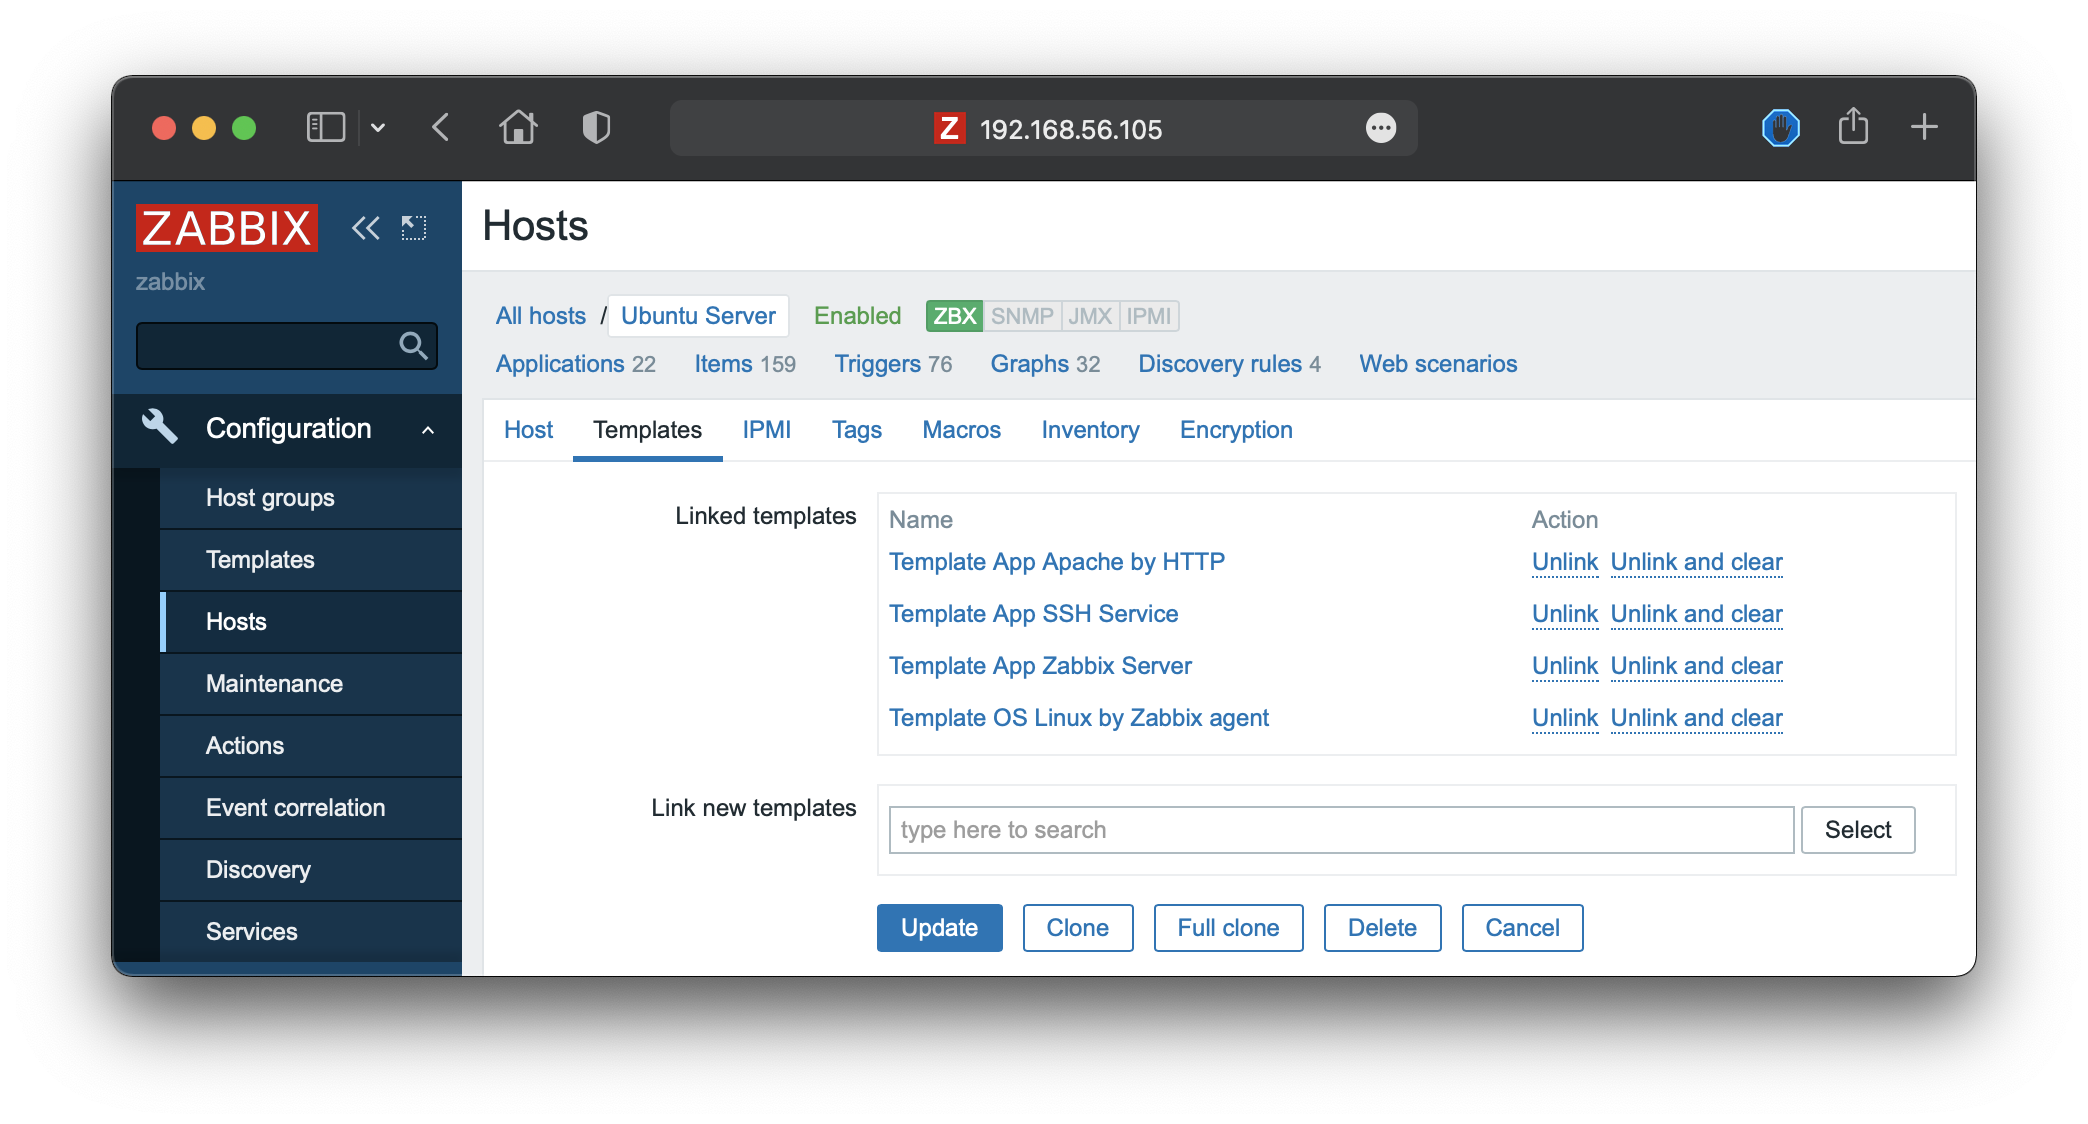
\includegraphics[scale=0.4225]{images/ubuntu_templates.png}
        \caption{Configuración apartado templates de Ubuntu Server}
        \label{fig:ubuntu_templates}
    \end{figure}
Una vez hemos rellenado los campos descritos anteriormente pulsamos el botón \textbf{\emph{Update}} para que se actualicen los campos.

\subsection{Configuración del servicio SSH}
Como el puerto del SSH es distinto al puerto por defecto, debemos indicarle al servicio SSH que nuestro puerto de SSH es el 22022. Para cambiar el puerto por defecto pulsamos
sobre el template \textbf{Template App SSH Service}, pulsamos sobre el apartado \textbf{Item} y por último, pulsamos sobre el apartado \textbf{SSH service is running}. Editamos
el apartado \textbf{key} de la siguiente forma:
    \begin{figure}[H]
        \centering
        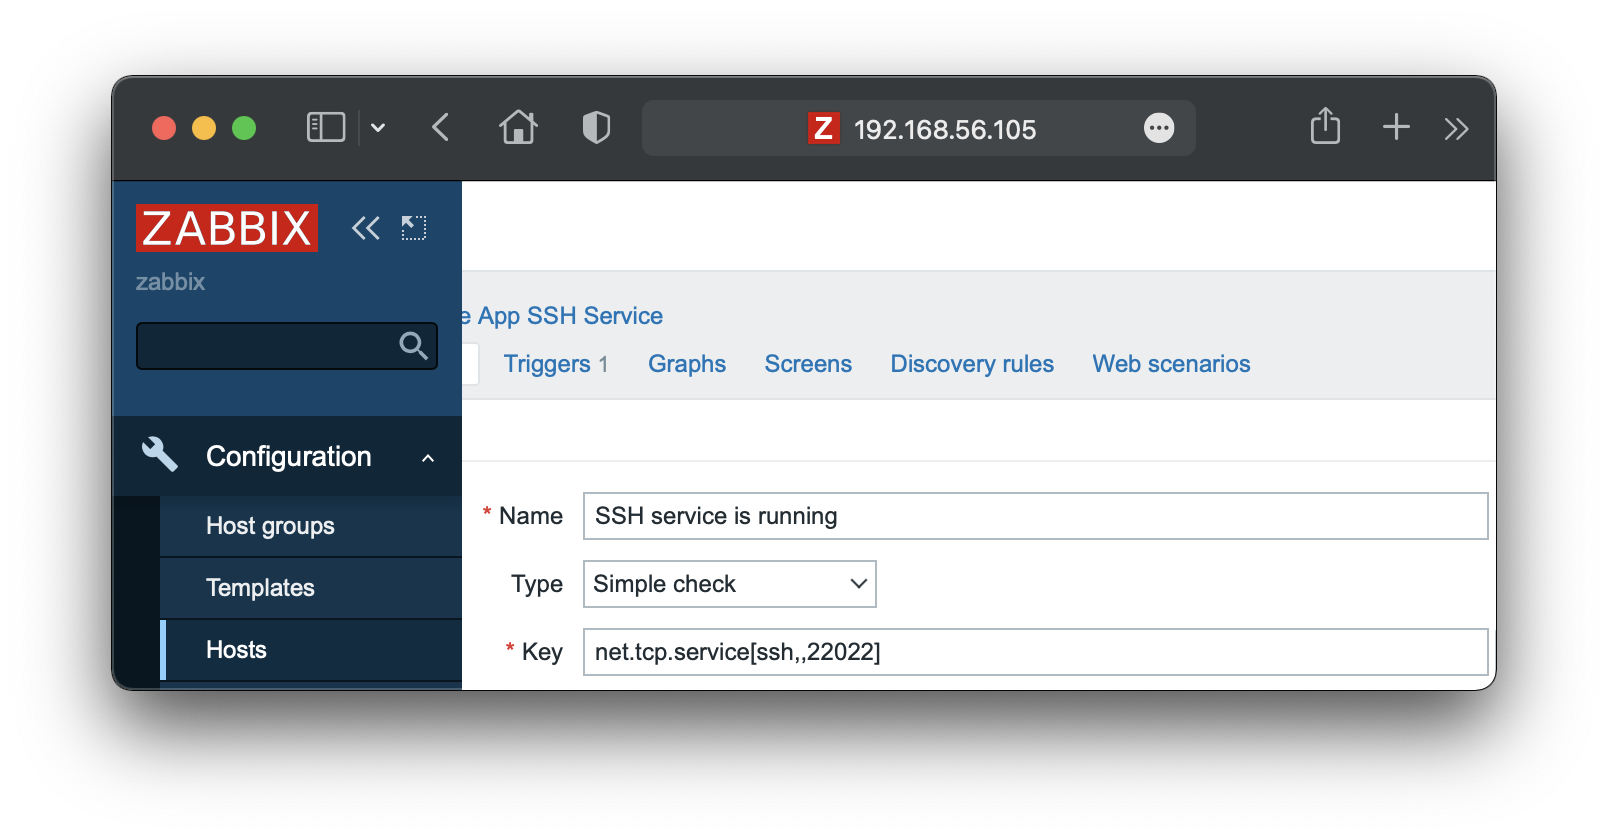
\includegraphics[scale=0.5]{images/ip_items.png}
        \caption{Configuración SSH en Zabbix}
        \label{fig:ip_items}
    \end{figure}
\subsection{Configuración del host CentOS}
\subsubsection{Apartado Host}
En este apartado definiremos el nombre con el que identificaremos la máquina con CentOS, el grupo al que pertenece, la IP de la máquina y el puerto de escucha. Rellenamos los campos
anteriores de la siguiente forma:
    \begin{itemize}
        \item \textbf{Host name:} CentOS
        \item \textbf{Groups:} Zabbix Servers
        \item \textbf{IP address:} 192.168.56.110
        \item \textbf{Port:} 10050
    \end{itemize}
    \begin{figure}[H]
        \centering
        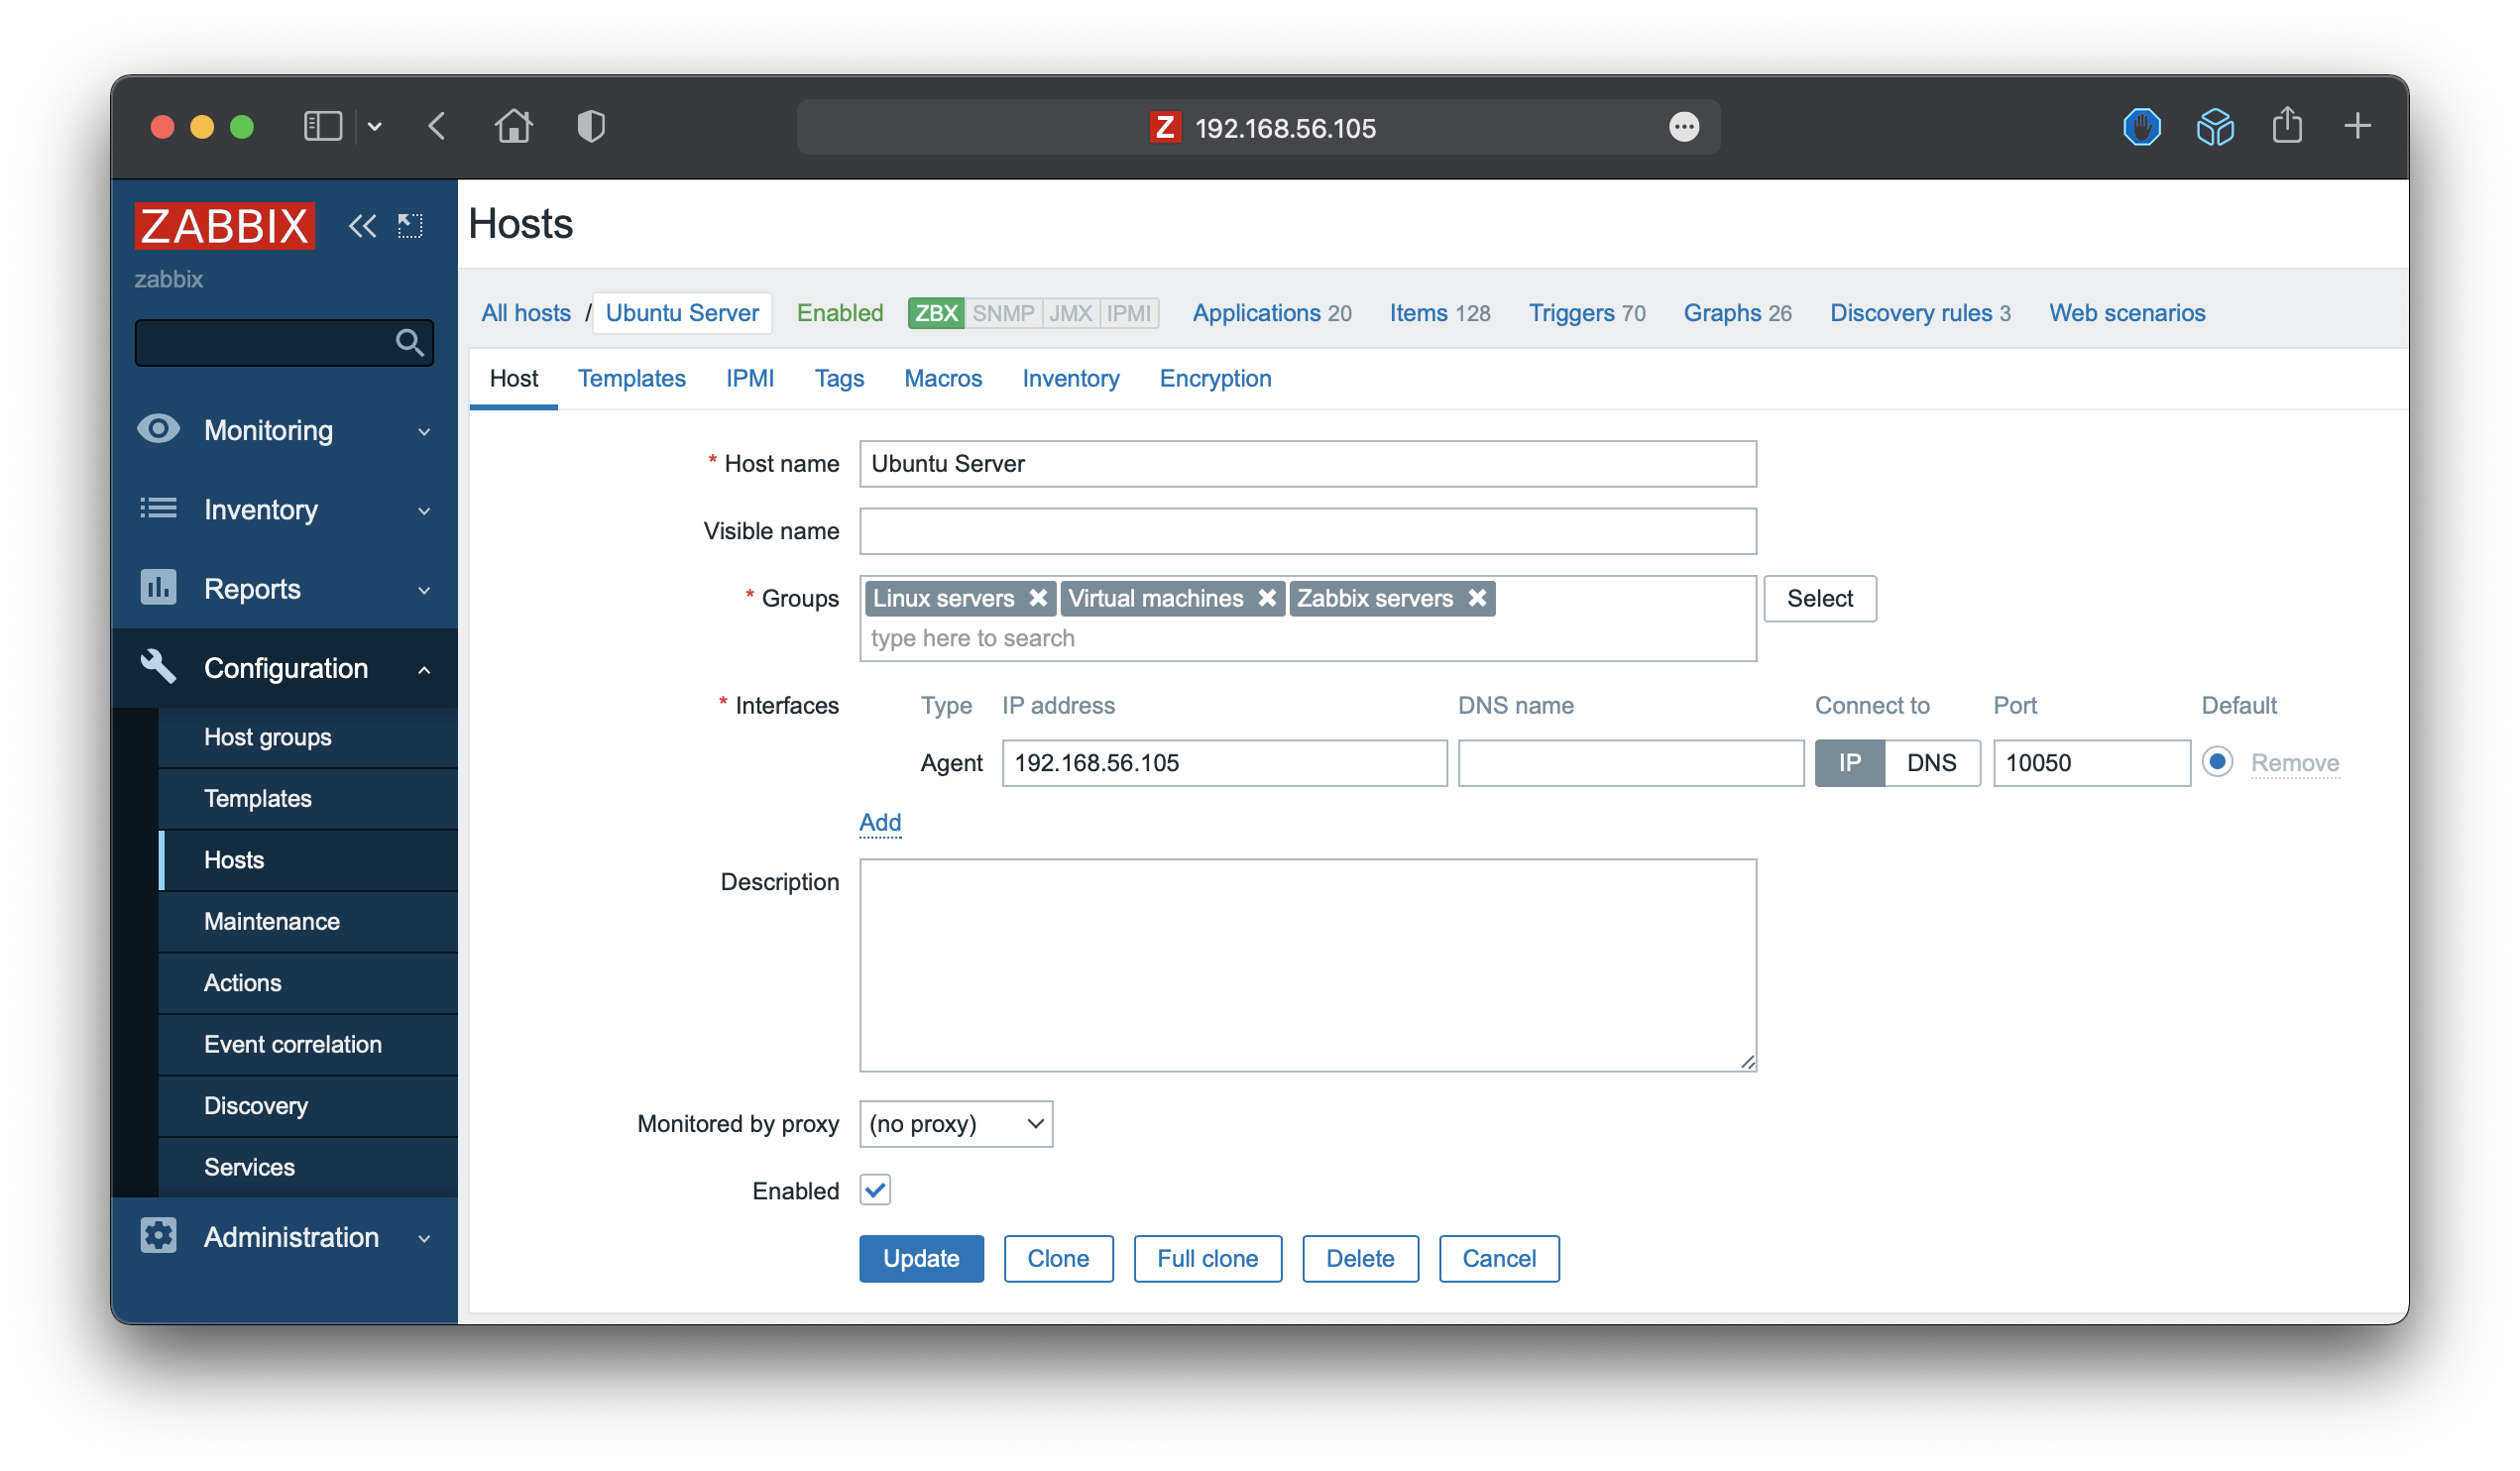
\includegraphics[scale=0.35]{images/centos_conf.png}
        \caption{Configuración apartado host de CentOS}
        \label{fig:centos_conf}
    \end{figure}
Una vez hemos rellenado los campos descritos anteriormente pulsamos el botón \textbf{\emph{Update}} para que se actualicen los campos.

\subsubsection{Apartado Templates}
En el apartado Templates añadimos los templates necesarios de forma que tenga enlazados los siguientes templates:
    \begin{itemize}
        \item \textbf{Template App Apache by HTTP:} para monitorizar el servicio HTTP
        \item \textbf{Template App SSH Service:} para monitorizar el servicio SSH
        \item \textbf{Template App Zabbix Server:} indicamos el servidor
    \end{itemize}
    \begin{figure}[H]
        \centering
        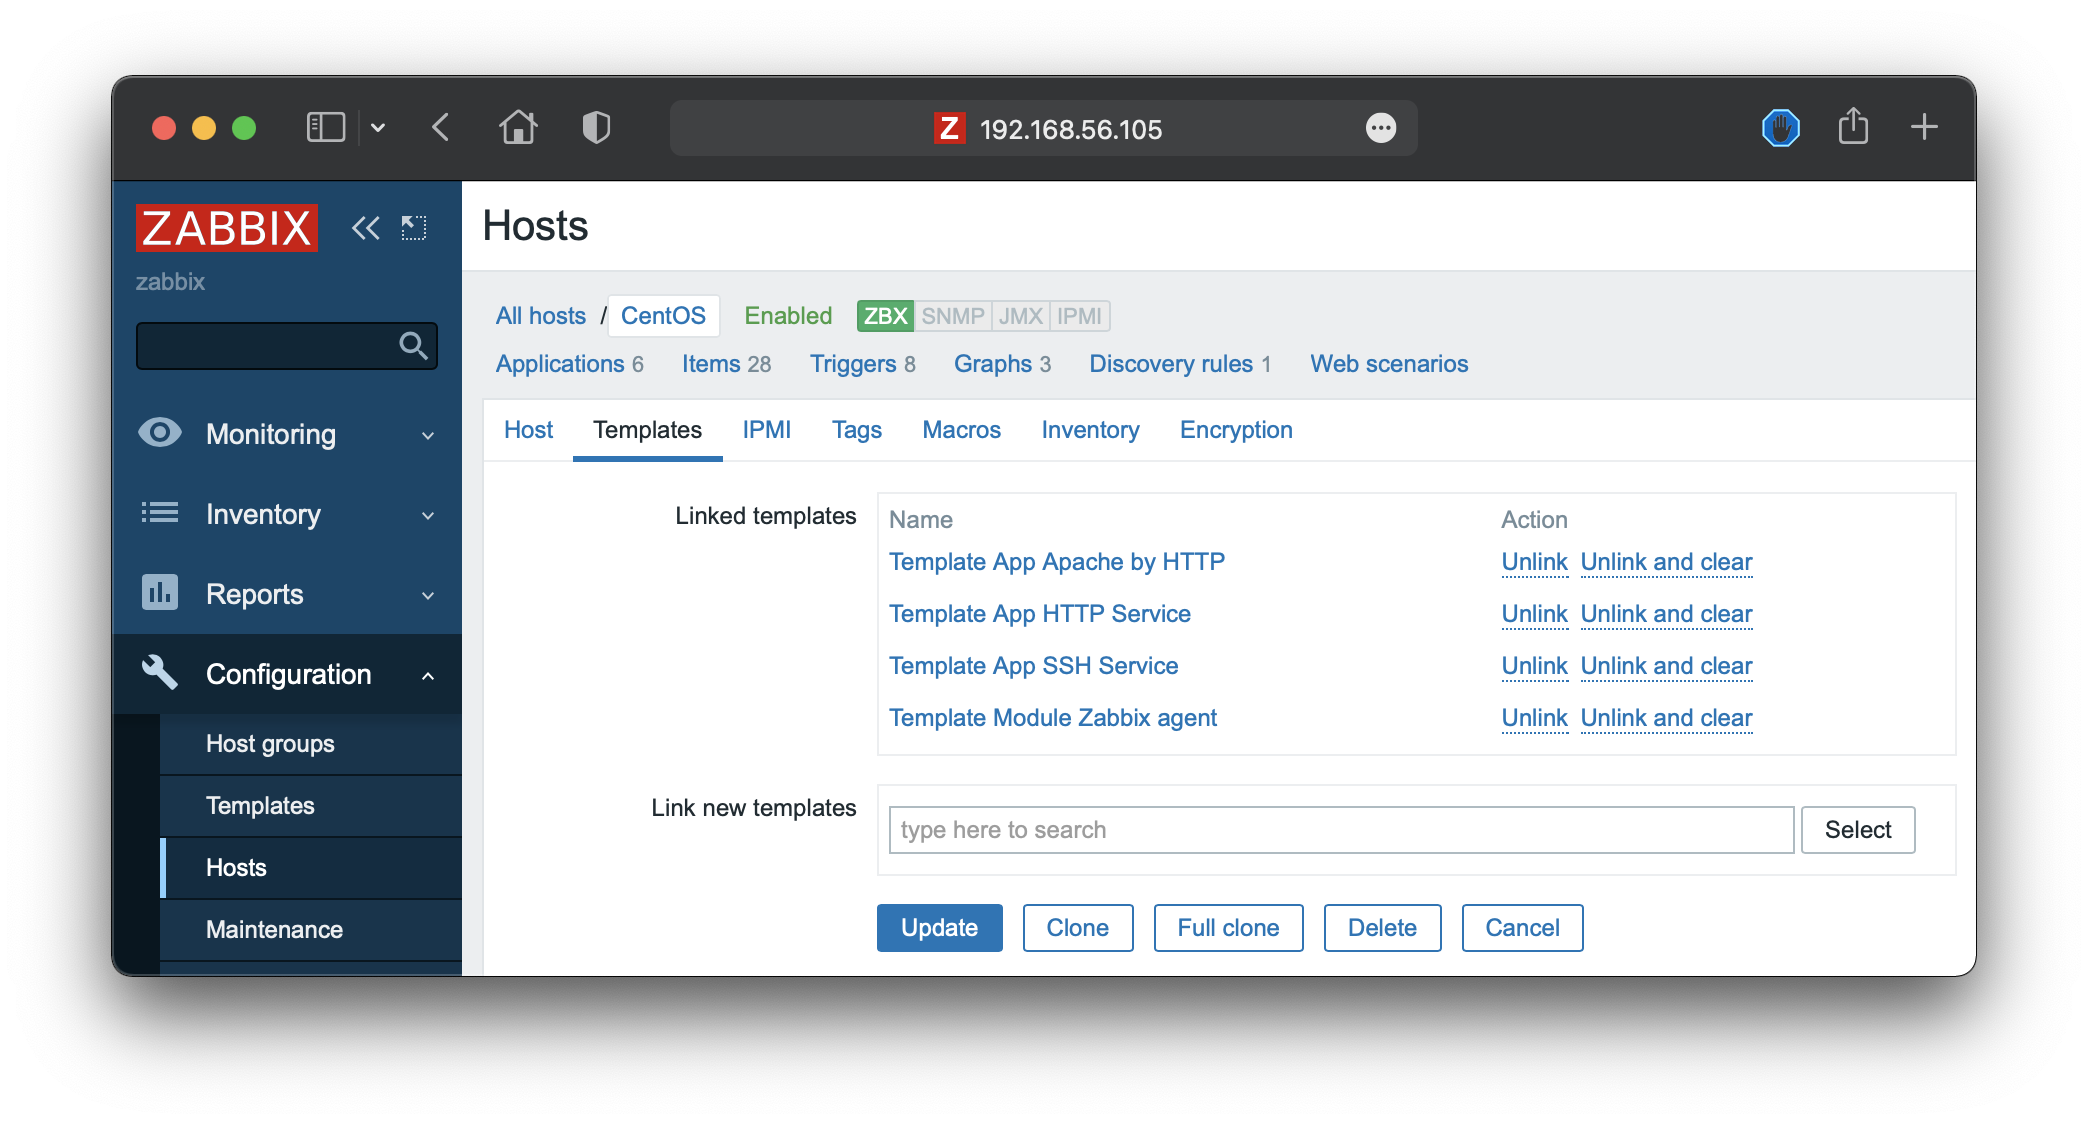
\includegraphics[scale=0.45]{images/centos_templates.png}
        \caption{Configuración apartado templates de CentOS}
        \label{fig:centos_templates}
    \end{figure}
Una vez hemos rellenado los campos descritos anteriormente pulsamos el botón \textbf{\emph{Update}} para que se actualicen los campos.

%%%%%%%%%%%%%%%%%%%%%%%%%%%%%%%%%%%%%%%%%%%%%%%%
% Apartado para la monitorizacación SSH y HTTP %
%%%%%%%%%%%%%%%%%%%%%%%%%%%%%%%%%%%%%%%%%%%%%%%%
\newpage
\section{Configuración para la monitorización de los servicios HTTP y SSH}
Para la monitorización de ambas máquinas creamos una \textbf{\emph{Dashboard}} para cada máquina. Para ello nos vamos a \textbf{\emph{Monitoring}} y en \textbf{\emph{Dashboard}} le damos
a crear nueva en el icono de las tres barras arriba a la derecha. Una vez hemos creado la \textbf{\emph{Dashboard}}, creamos los widgets que creamos convenientes pulsando sobre
\textbf{\emph{Add widget}}. Crearé un reloj como ejemplo:
    \begin{figure}[H]
        \centering
        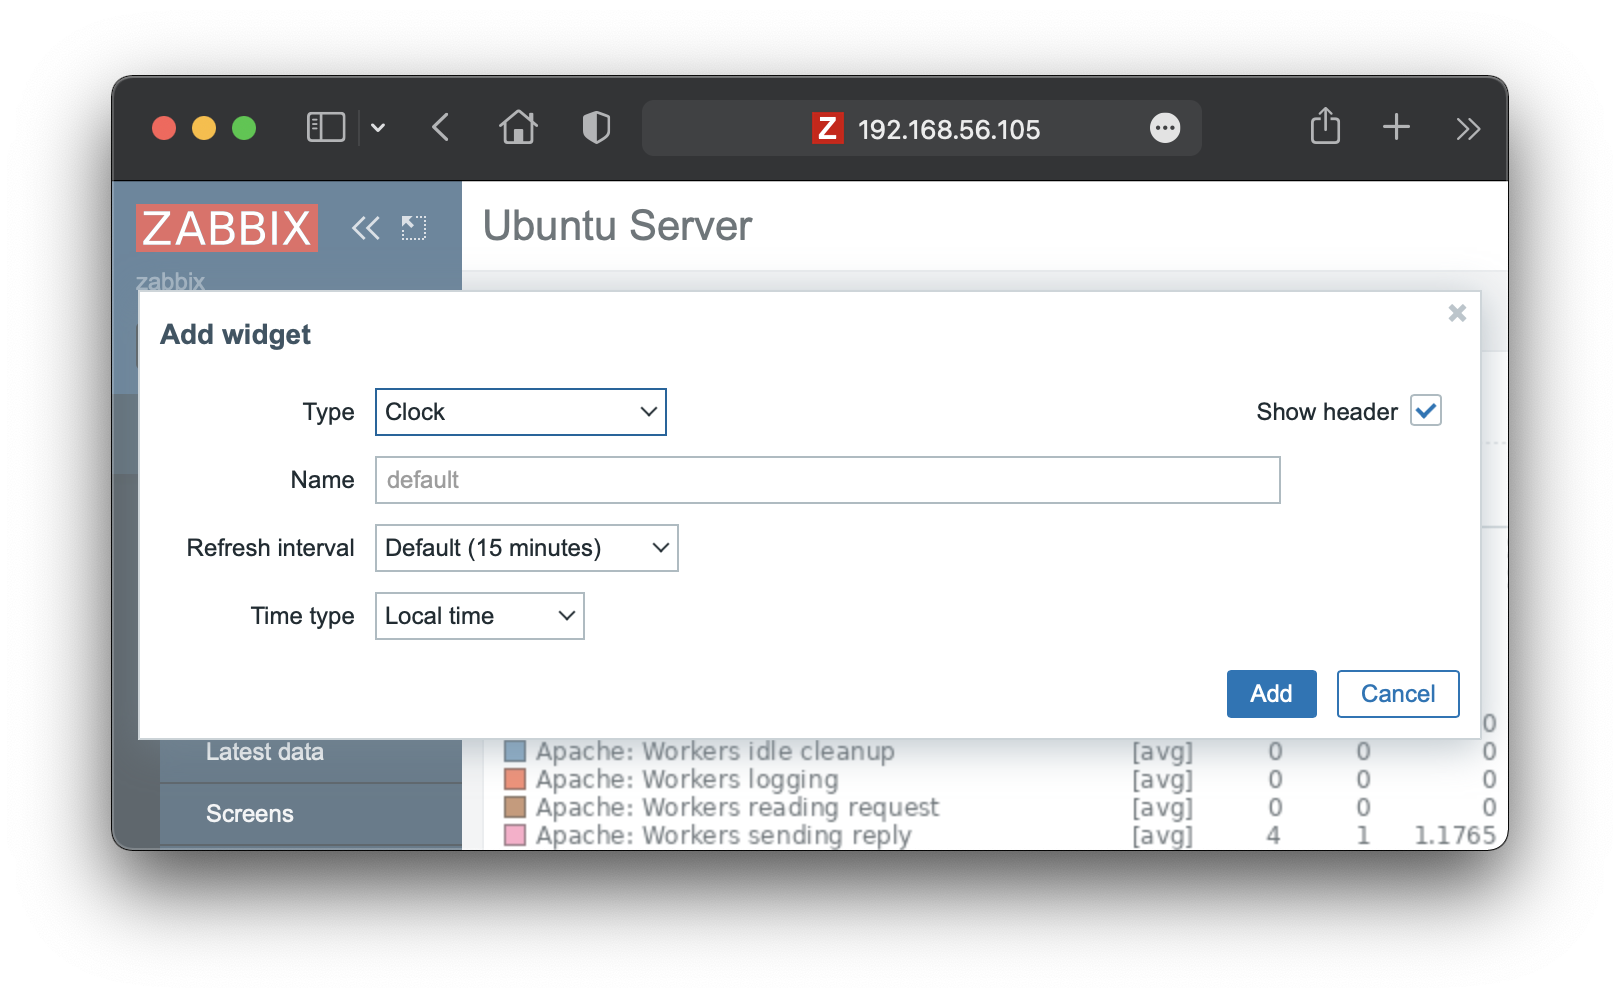
\includegraphics[scale=0.3]{images/widget.png}
        \caption{Creación de un widget}
        \label{fig:widget}
    \end{figure}

\subsection{Monitorización en Ubuntu Server}
Tras crear unos cuantos widgets esta es la \textbf{\emph{Dashboard}} que ha quedado para la monitorización de Ubuntu Server.
    \begin{figure}[H]
        \centering
        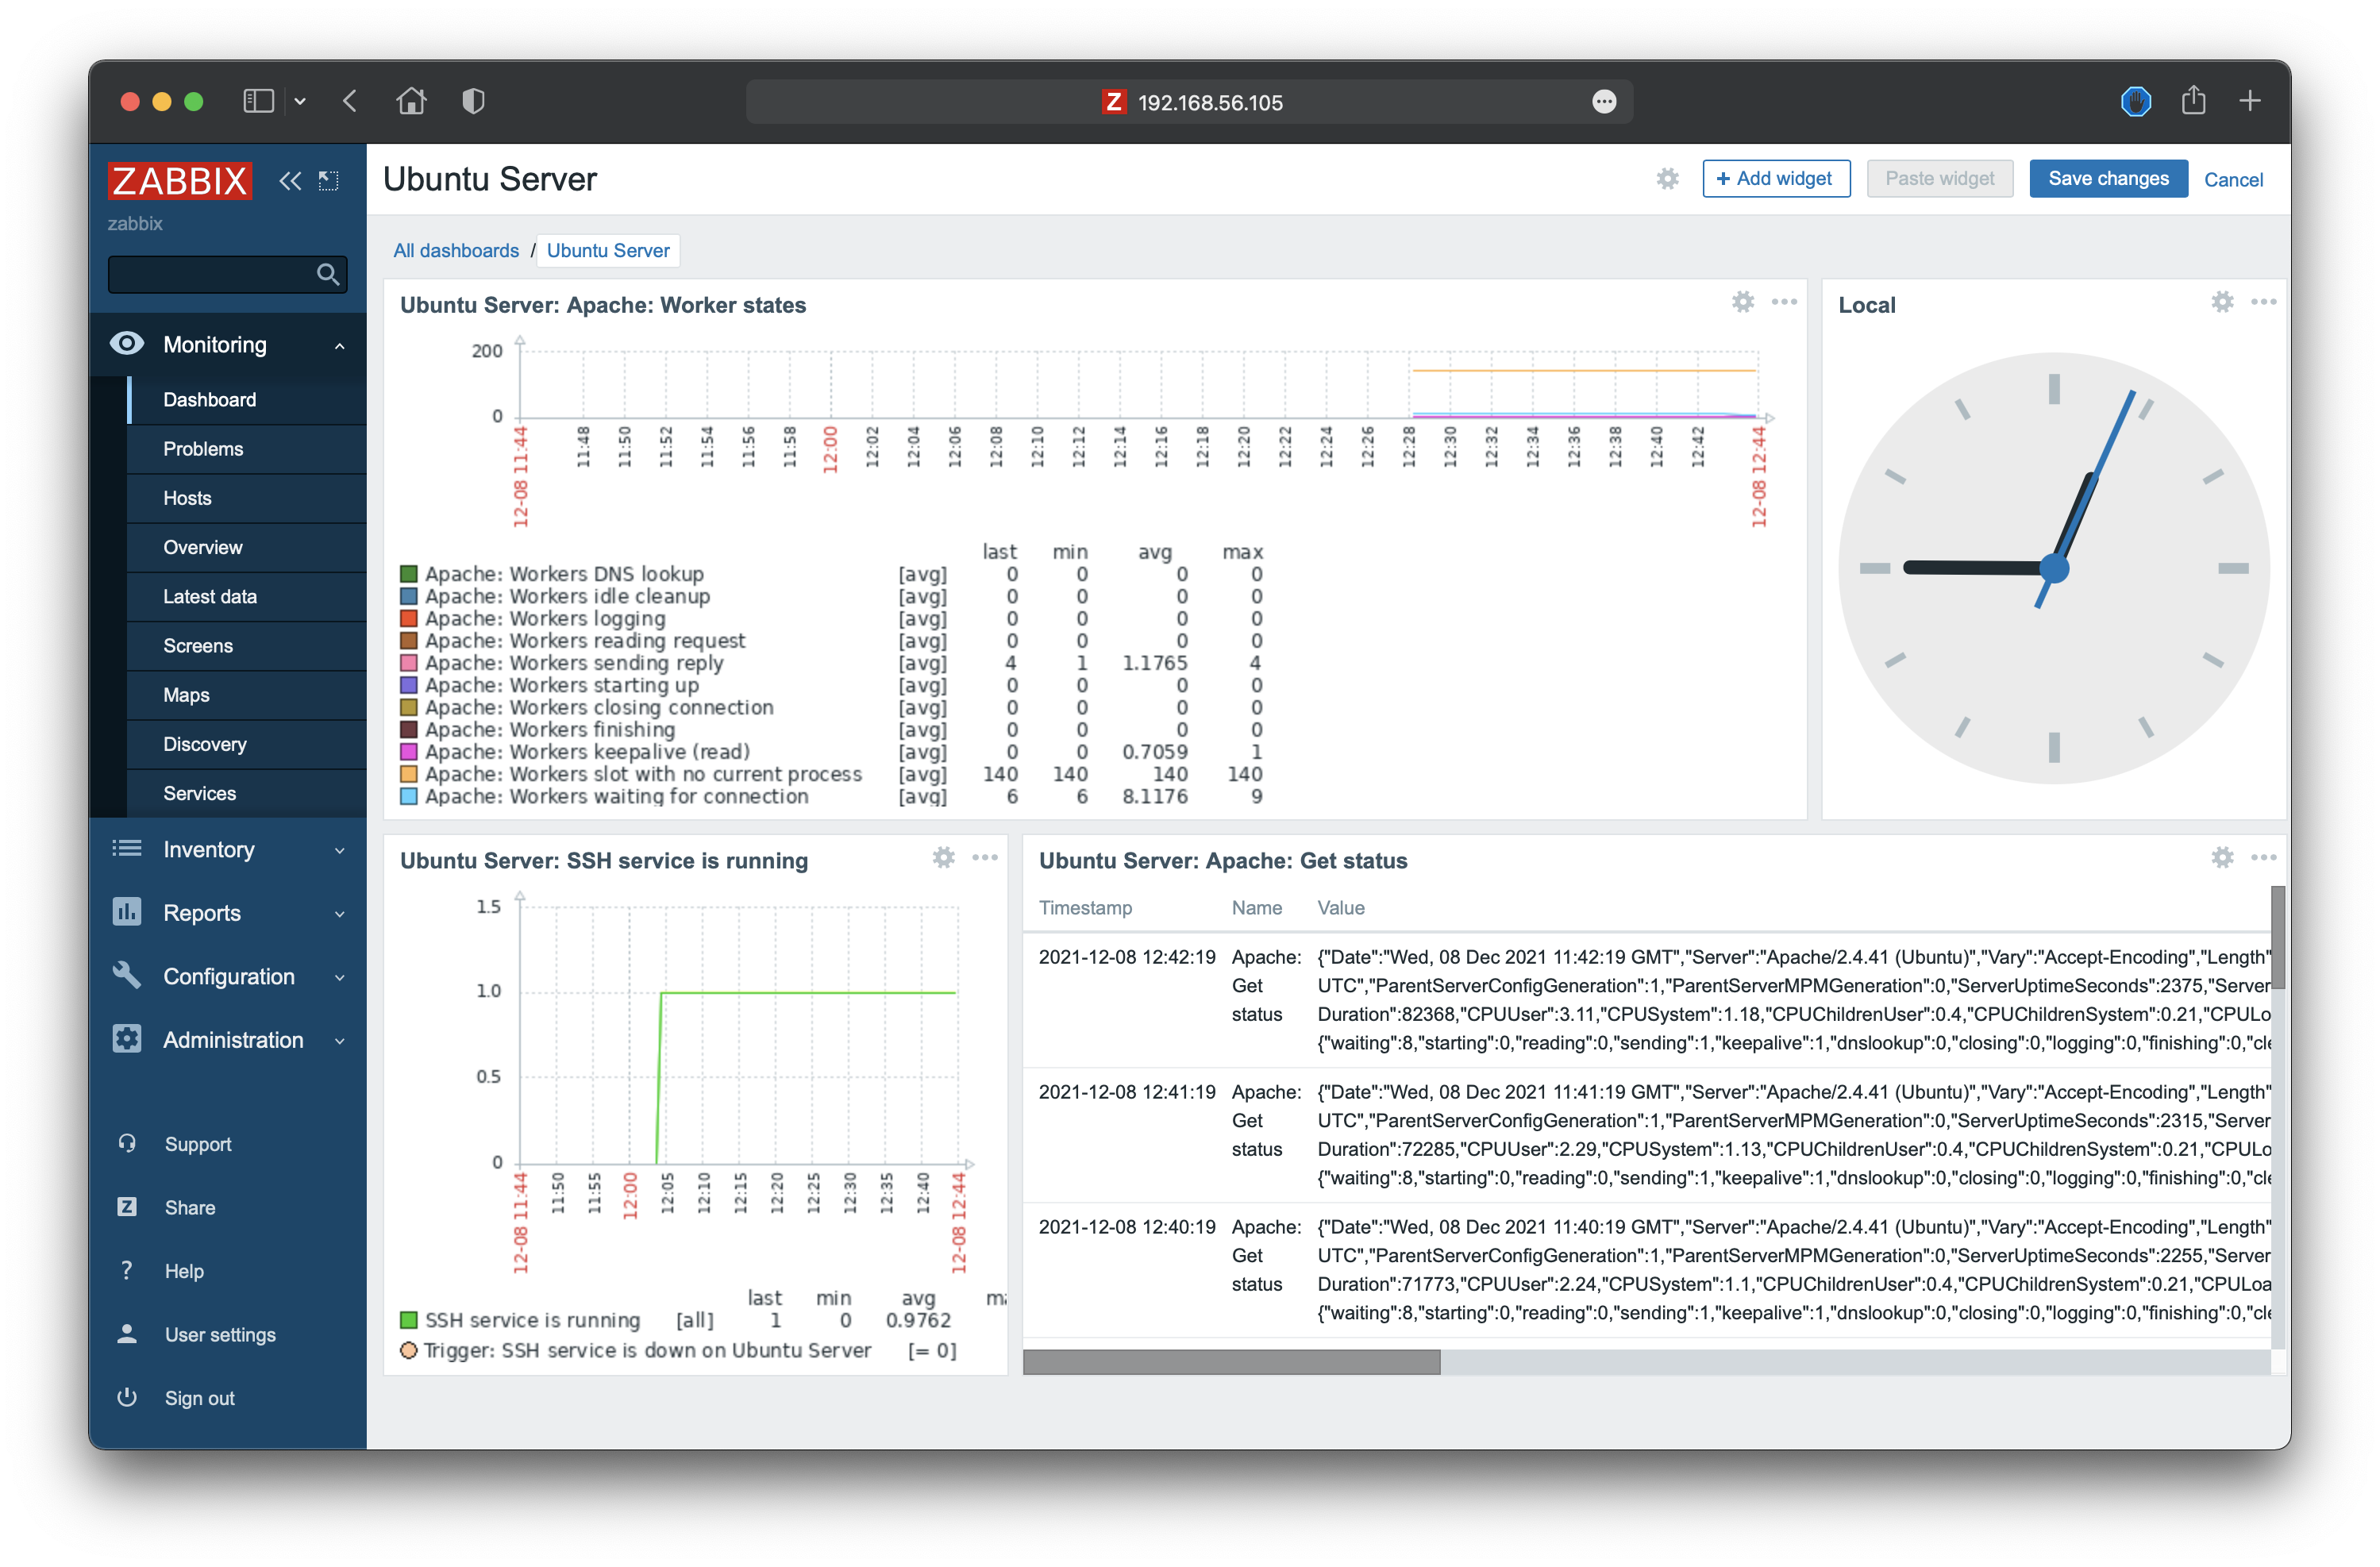
\includegraphics[scale=0.275]{images/ubuntu_dashboard.png}
        \caption{Dashboard de ubuntu}
        \label{fig:ubuntu_dashboard}
    \end{figure}

\subsection{Monitorización en CentOS}
Creamos la misma \textbf{\emph{Dashboard}} que hemos usado para la monitorización de Ubuntu Server. He apagado el servicio SSHD en CentOS para comprobar
que funciona bien la monitorización.
    \begin{figure}[H]
        \centering
        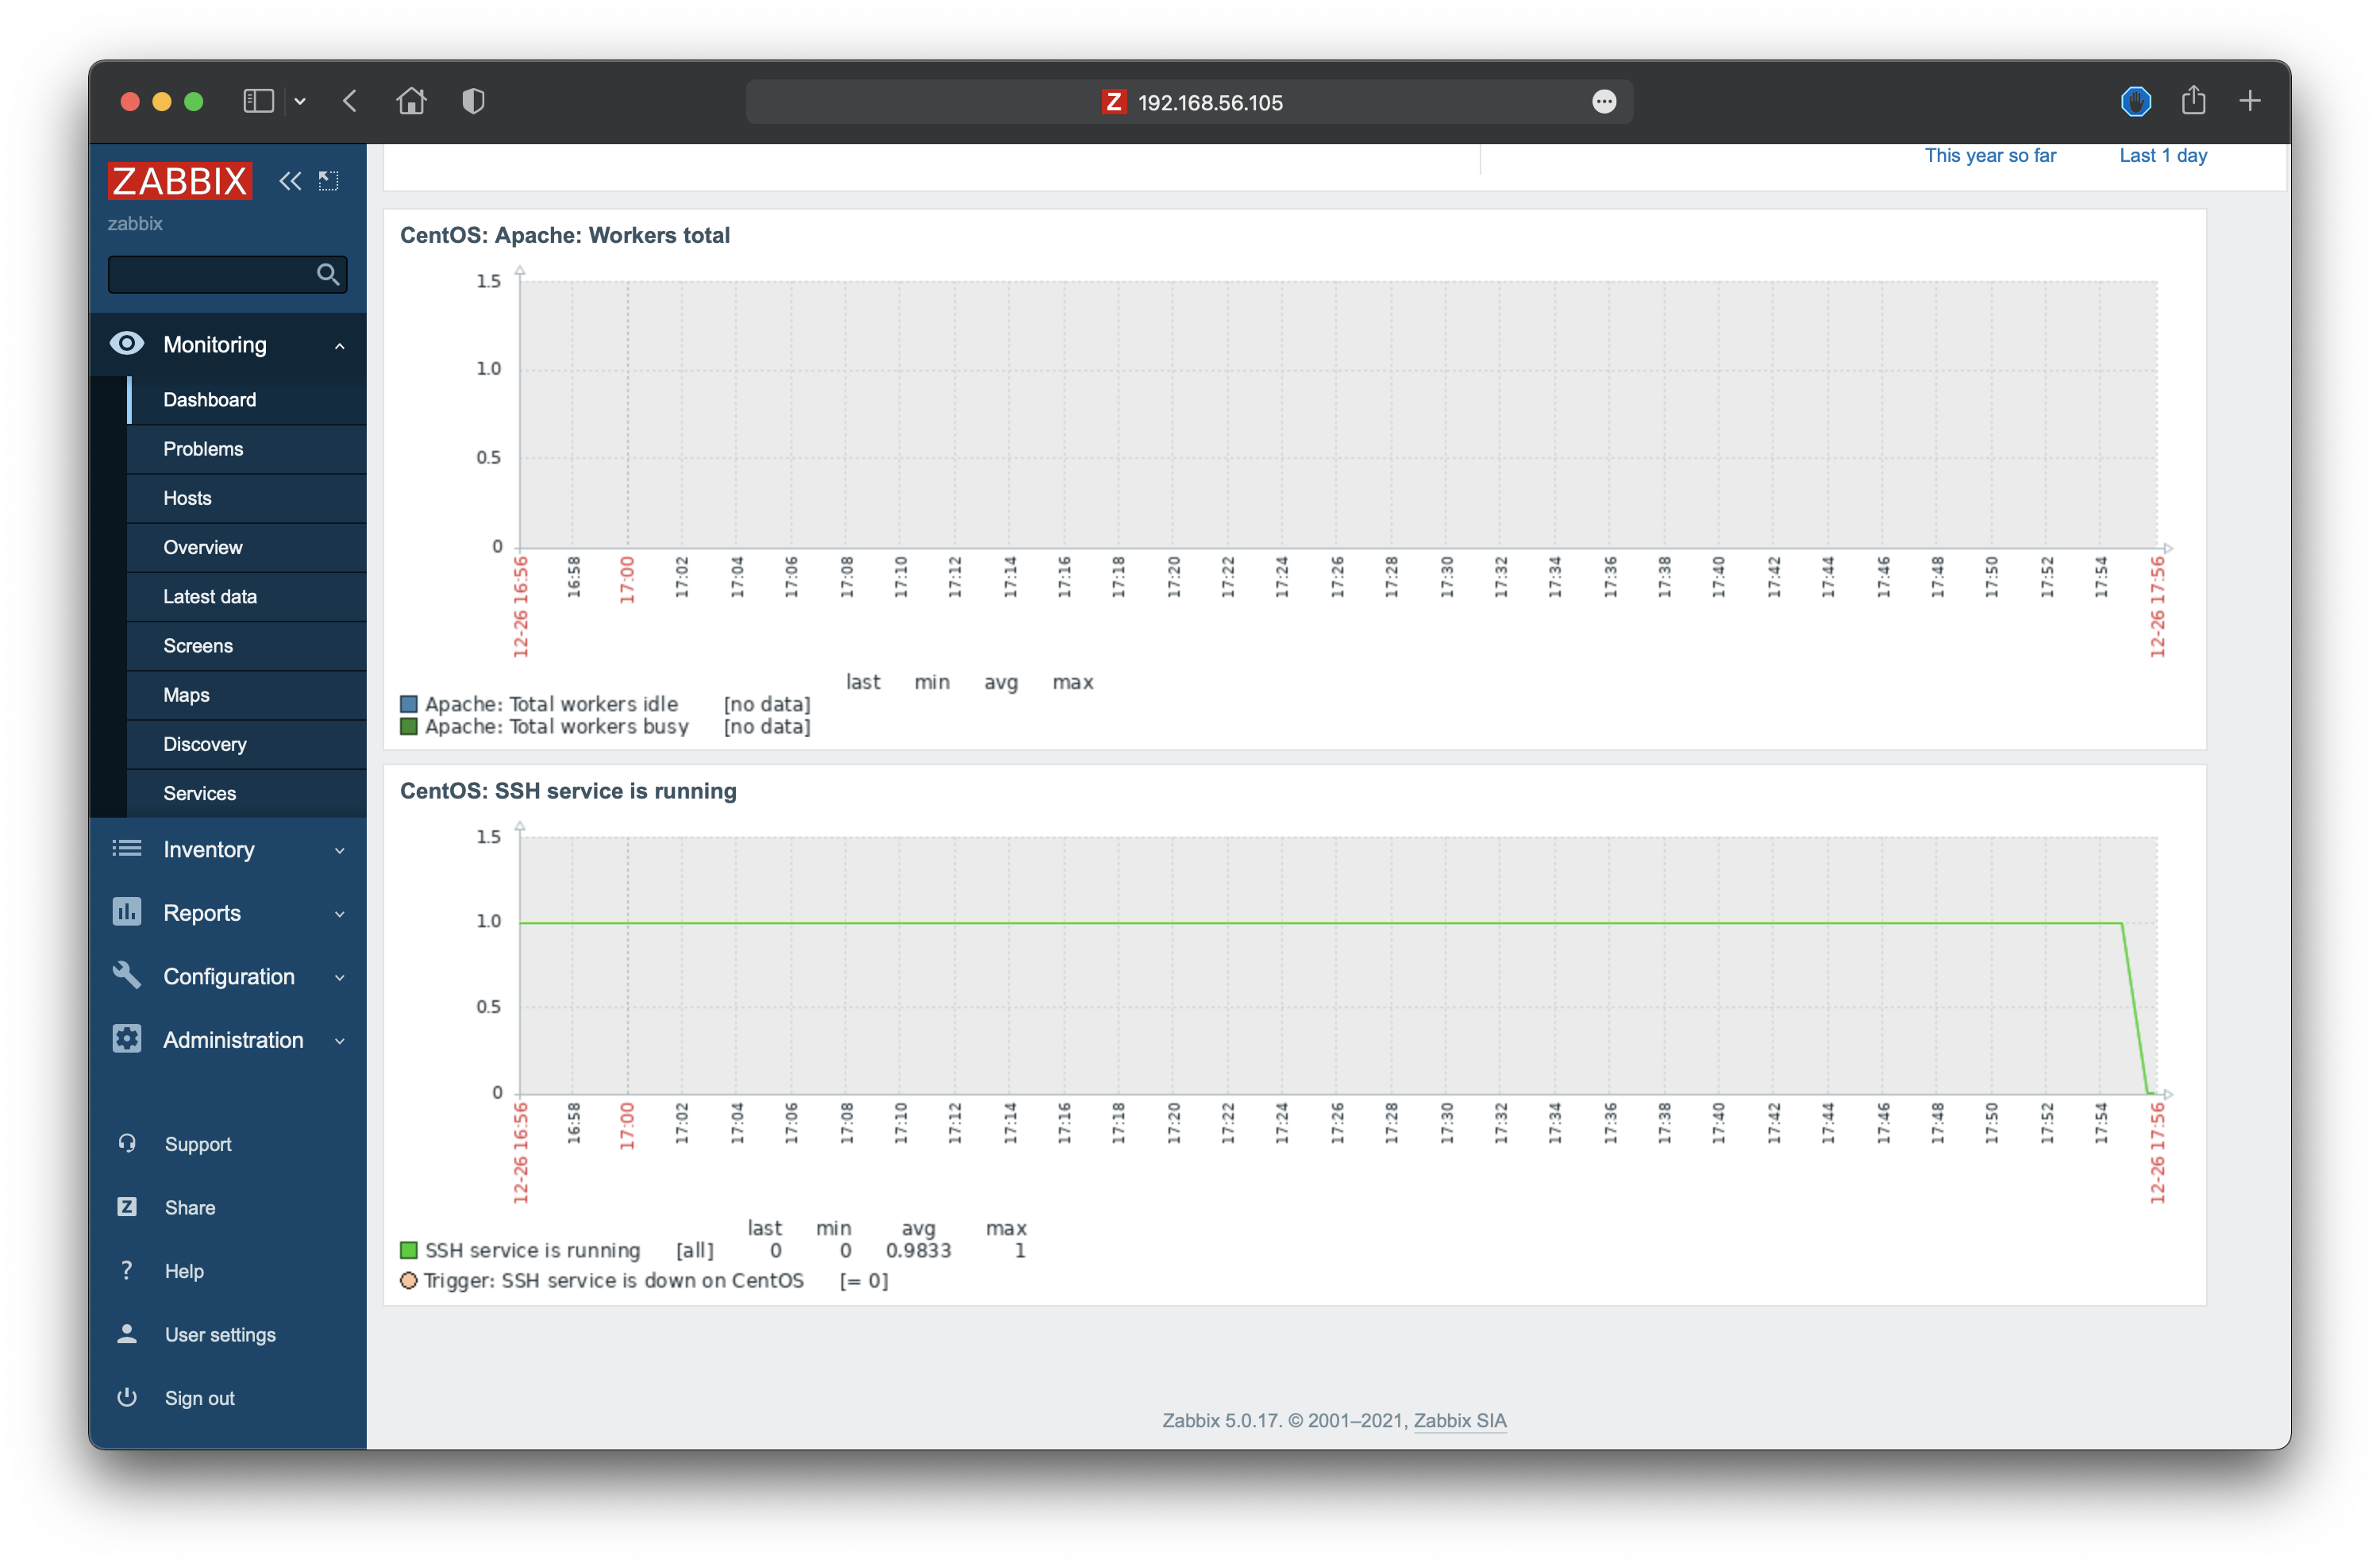
\includegraphics[scale=0.275]{images/centOS_dashboard.png}
        \caption{Dashboard de centOS}
        \label{fig:centOS_dashboard}
    \end{figure}

%%%%%%%%%%%%%%%%%%%%%%%%%%%%%%%%%%%%%%%%%%%%%
% Apartado para la configuracion de Ansible %
%%%%%%%%%%%%%%%%%%%%%%%%%%%%%%%%%%%%%%%%%%%%%
\newpage
\section{Instalación de Ansible}
\subsection{Instalación de Ansible en Ubuntu Server}
Ubuntu Server va a ser la máquina que monitorizará los RAID1 tanto de Ubuntu Server como de CentOS. Para llevar a cabo esta
monitorización lo primero que debemos hacer es instalar ansible en Ubuntu Server.

Instalamos ansible con el siguiente comando:
\begin{tcolorbox}[colback=black!10, halign=left]
    \$ sudo apt install ansible
\end{tcolorbox}
Una vez se ha instalado, cambiamos el puerto por el que accede al servicio SSH ya que lo cambiamos al 22022. Para ello editamos
el archivo ubicado en \textbf{/etc/ansible/ansible.cfg} descomentamos la variable \textbf{\emph{remote\_ports}} y le asignamos el valor \textbf{\emph{22022}}.
    \begin{tcolorbox}[colback=black!10, halign=left]
        \$ sudo vi /etc/ansible/ansible.cfg
    \end{tcolorbox}
    \begin{figure}[H]
        \centering
        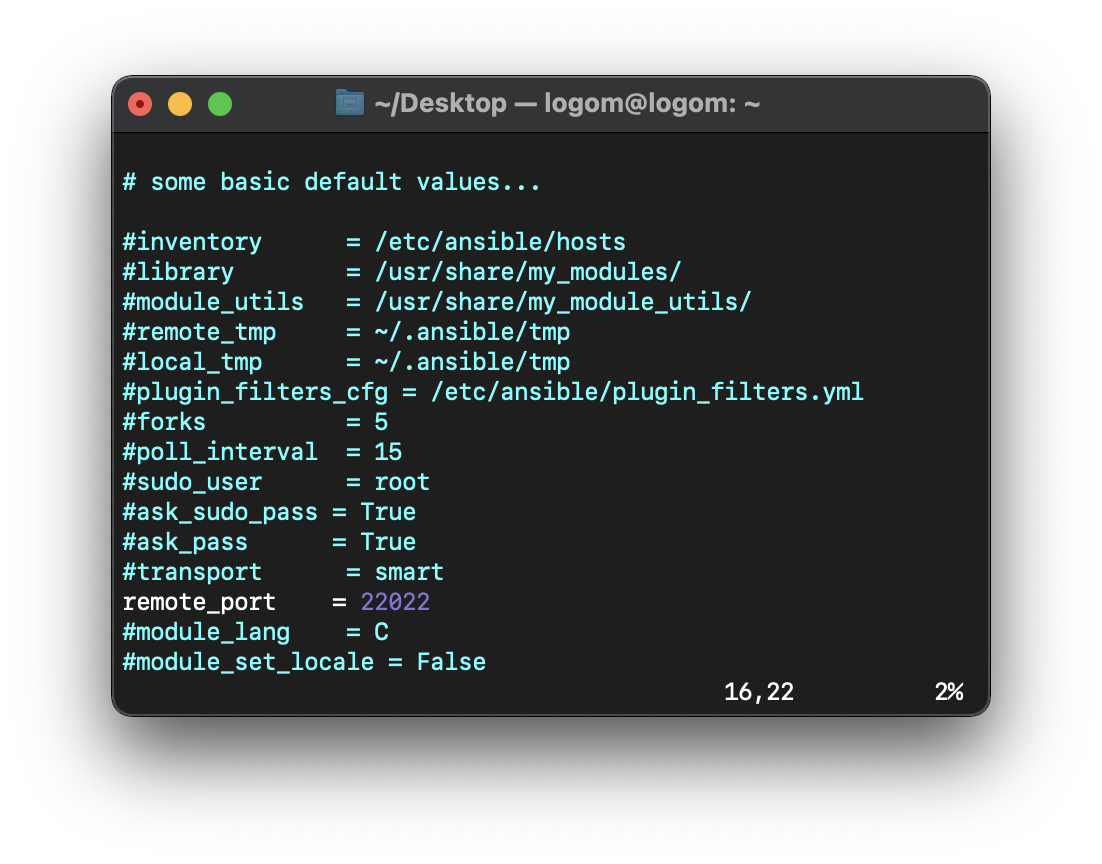
\includegraphics[scale=0.75]{images/ansible_cfg.png}
        \caption{Archivo de configuración de Ansible}
        \label{fig:ansible_cfg}
    \end{figure}

\subsection{Configuración de Ansible}
Lo siguiente que tenemos que hacer es configurar el archivo donde Ansible lee las IP de las máquinas a las que les tiene que mandar las órdenes. Este archivo
se encuentra en \textbf{/etc/ansible/hosts} y añadimos las IP’s de Ubuntu Server y CentOS.
    \begin{tcolorbox}[colback=black!10, halign=left]
        \$ sudo vi /etc/ansible/hosts
    \end{tcolorbox}
    \begin{figure}[H]
        \centering
        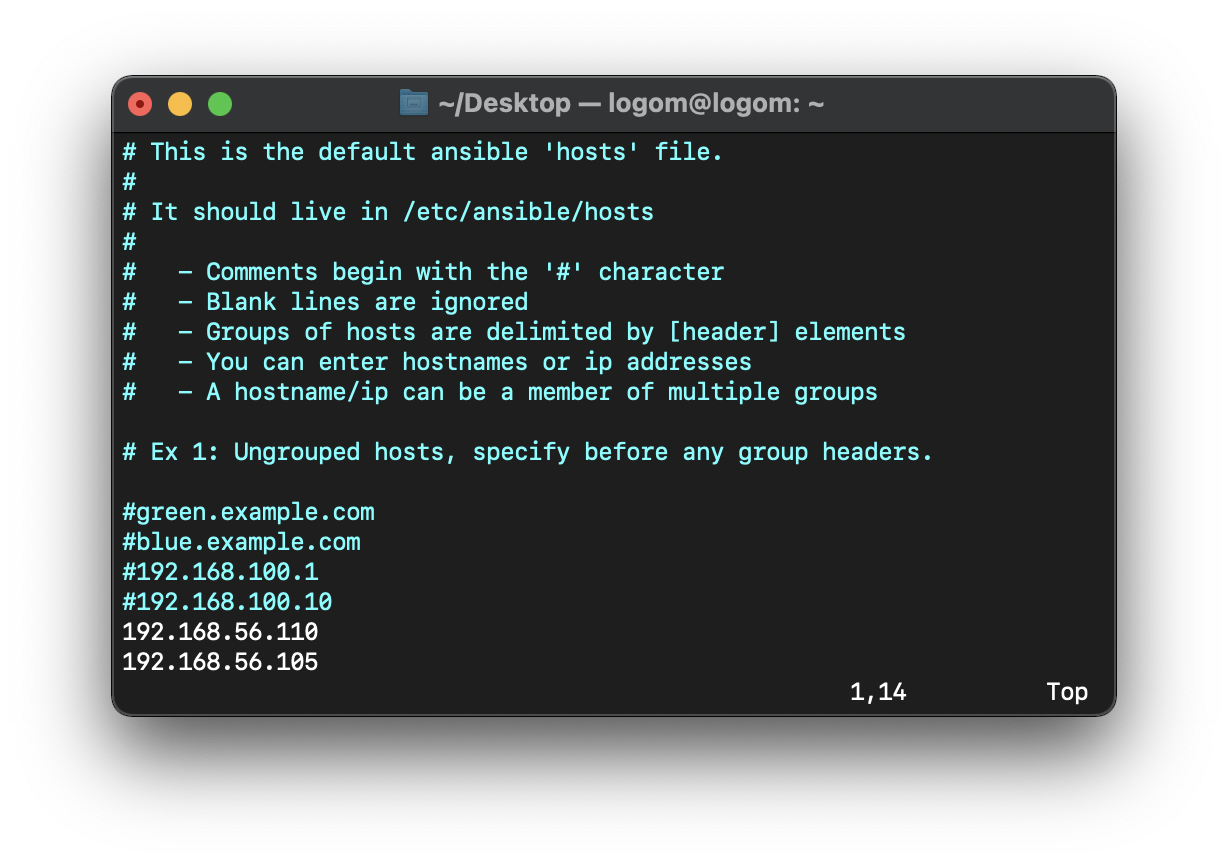
\includegraphics[scale=0.75]{images/ansible_hosts.png}
        \caption{Archivo de configuración de hosts de Ansible}
        \label{fig:ansible_hosts}
    \end{figure}

\subsection{Configuración de las claves públicas y privadas}
Ansible necesita tener acceso por SSH a las máquinas a las que va a mandar órdenes por lo tanto es necesario que estén habilitadas las claves públicas y
privadas. Por lo tanto las habilitamos para ambas máquinas desde Ubuntu Server.

Ubuntu Server:
    \begin{tcolorbox}[colback=black!10, halign=left]
        \$ ssh-keygen
    \end{tcolorbox}
    \begin{tcolorbox}[colback=black!10, halign=left]
        \$ ssh-copy-id logom@192.168.56.105 -p 22022
    \end{tcolorbox}

CentOS:
    \begin{tcolorbox}[colback=black!10, halign=left]
        \$ ssh-copy-id logom@192.168.56.110 -p 22022
    \end{tcolorbox}

\subsection{Comprobación funcionamiento de Ansible}
Comprobamos que todo funciona correctamente enviando un ping a todas las máquinas:
    \begin{tcolorbox}[colback=black!10, halign=left]
        \$ ansible all -m ping -u logom
    \end{tcolorbox}

Si todo funciona correctamente debe aparecer una imagen similar a esta:
    \begin{figure}[H]
        \centering
        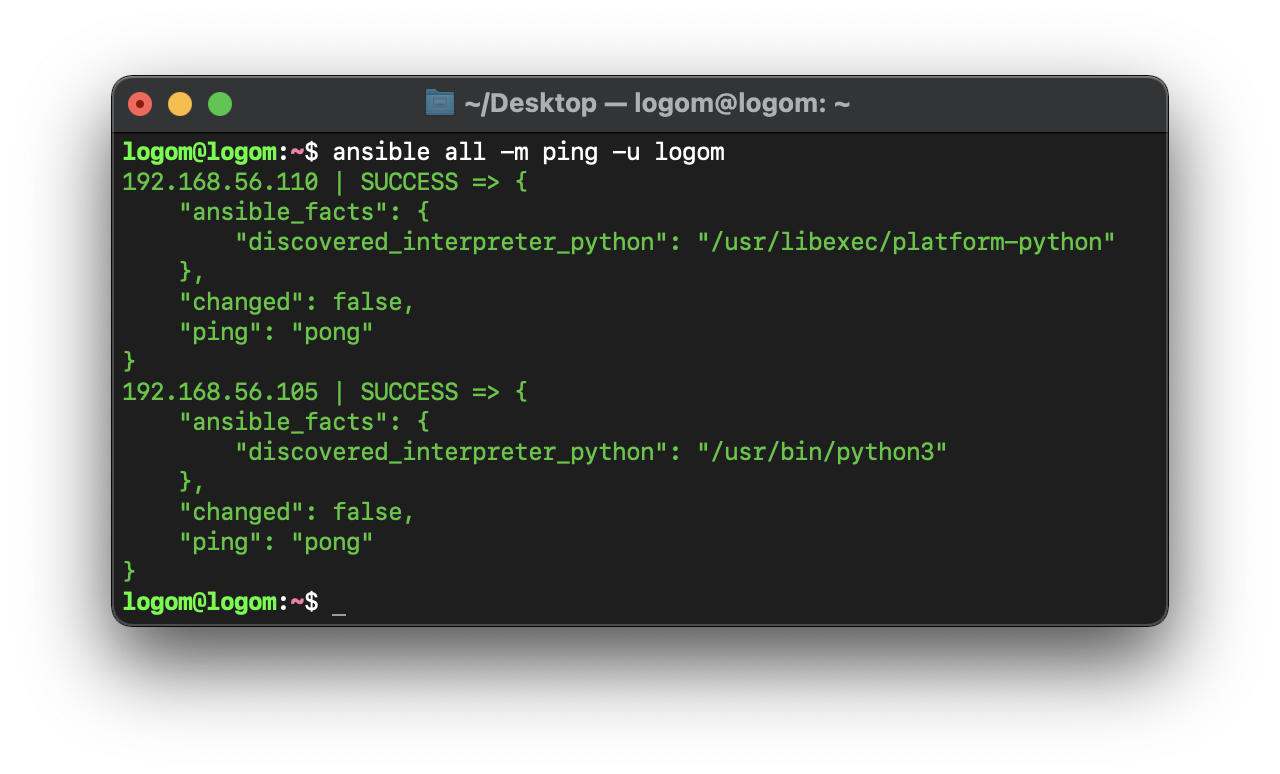
\includegraphics[scale=0.5]{images/ansible_ping.png}
        \caption{Ping correcto con Ansible}
        \label{fig:ansible_ping}
    \end{figure}

Una vez sabemos que todo funciona correctamente, procedemos a crear un script básico de monitorización con Python. Lo creamos en nuestra carpeta de usuario.
    \begin{tcolorbox}[colback=black!10, halign=left]
        \$ vi mon\_raid.py
    \end{tcolorbox}

\subsection{Script de monitorización}
El código del script será el siguiente:
    \begin{figure}[H]
        \centering
        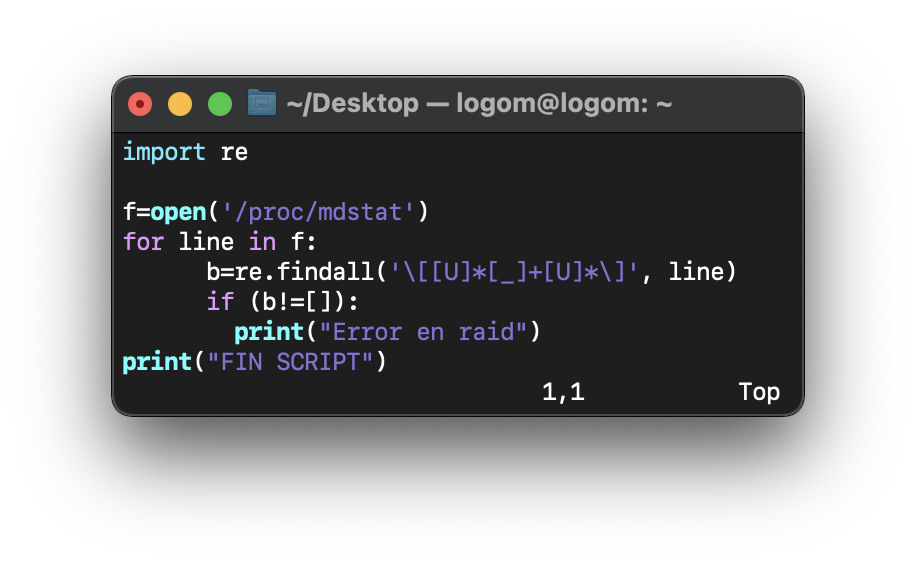
\includegraphics[scale=0.5]{images/mon_raid.png}
        \caption{Script de monitorización de Ansible}
        \label{fig:mon_raid}
    \end{figure}

Una vez tenemos copiado el script, lo enviamos a las máquinas que no lo tengan, en mi caso CentOS, con el siguiente comando:
    \begin{tcolorbox}[colback=black!10, halign=left]
        \$ scp -P 22022 mon\_raid.py logom@192.168.56.110:/home/logom/mon\_raid.py
    \end{tcolorbox}

Comprobamos que se haya enviado bien a CentOS y que tiene el mismo contenido. Si todo está bien procedemos a ejecutar el script en todas las máquinas:
    \begin{tcolorbox}[colback=black!10, halign=left]
        \begin{verbatim}$ ansible all -a "python3 ~/mon_raid.py" -u logom \end{verbatim}
    \end{tcolorbox}

Tras la ejecución del script, muestra para cada máquina a la que se lanzan órdenes si los RAIDS son correctos. En mi caso muestra que en CentOS está
todo correcto y en Ubuntu indica que en ambos RAIDS hay algún error.
    \begin{figure}[H]
        \centering
        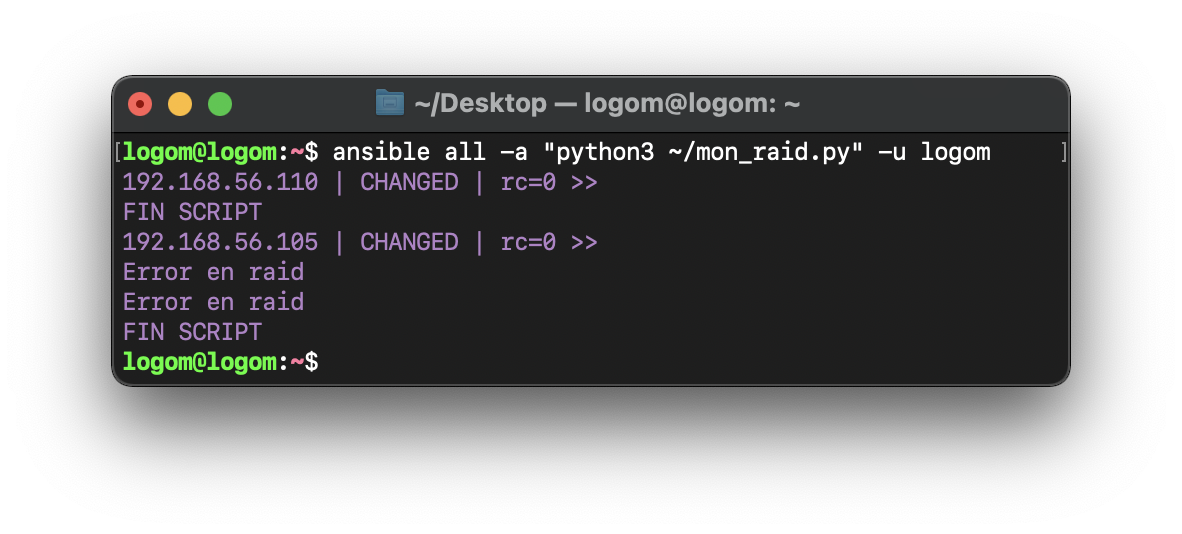
\includegraphics[scale=0.6]{images/ejecucion_script.png}
        \caption{Ejecución del script de monitorización de Ansible}
        \label{fig:ejecucion_script}
    \end{figure}

\subsection{Playbook}
Los playbooks son ficheros YAML. Crearemos un playbook para hacer un ping a las máquinas. Para ello creamos un archivo
yml como el de la siguiente imagen.
    \begin{tcolorbox}[colback=black!10, halign=left]
        \$ vi playbook.yml
    \end{tcolorbox}

    \begin{figure}[H]
        \centering
        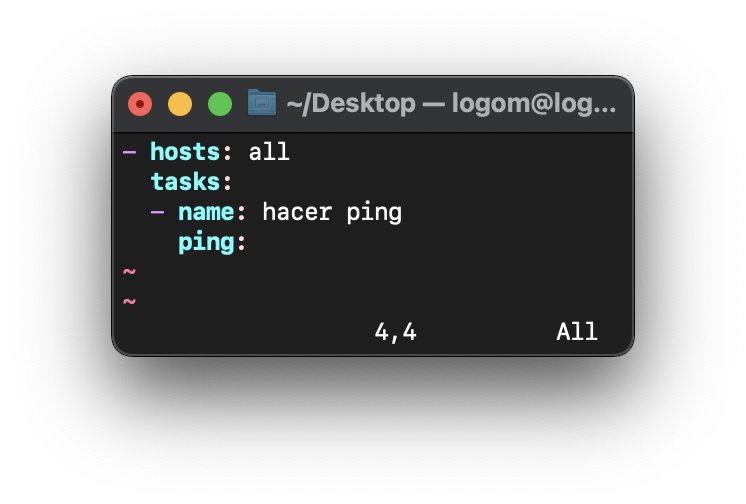
\includegraphics[scale=0.5]{images/playbook.png}
        \caption{Playbook de ansible}
        \label{fig:playbook}
    \end{figure}

Una vez hemos creado el playbook lo ejecutamos.
    \begin{tcolorbox}[colback=black!10, halign=left]
        \$ ansible-playbook playbook.yml
    \end{tcolorbox}

Una vez lo hayamos ejecutado, debería salir en la terminal algo similar a la siguiente imagen.
    \begin{figure}[H]
        \centering
        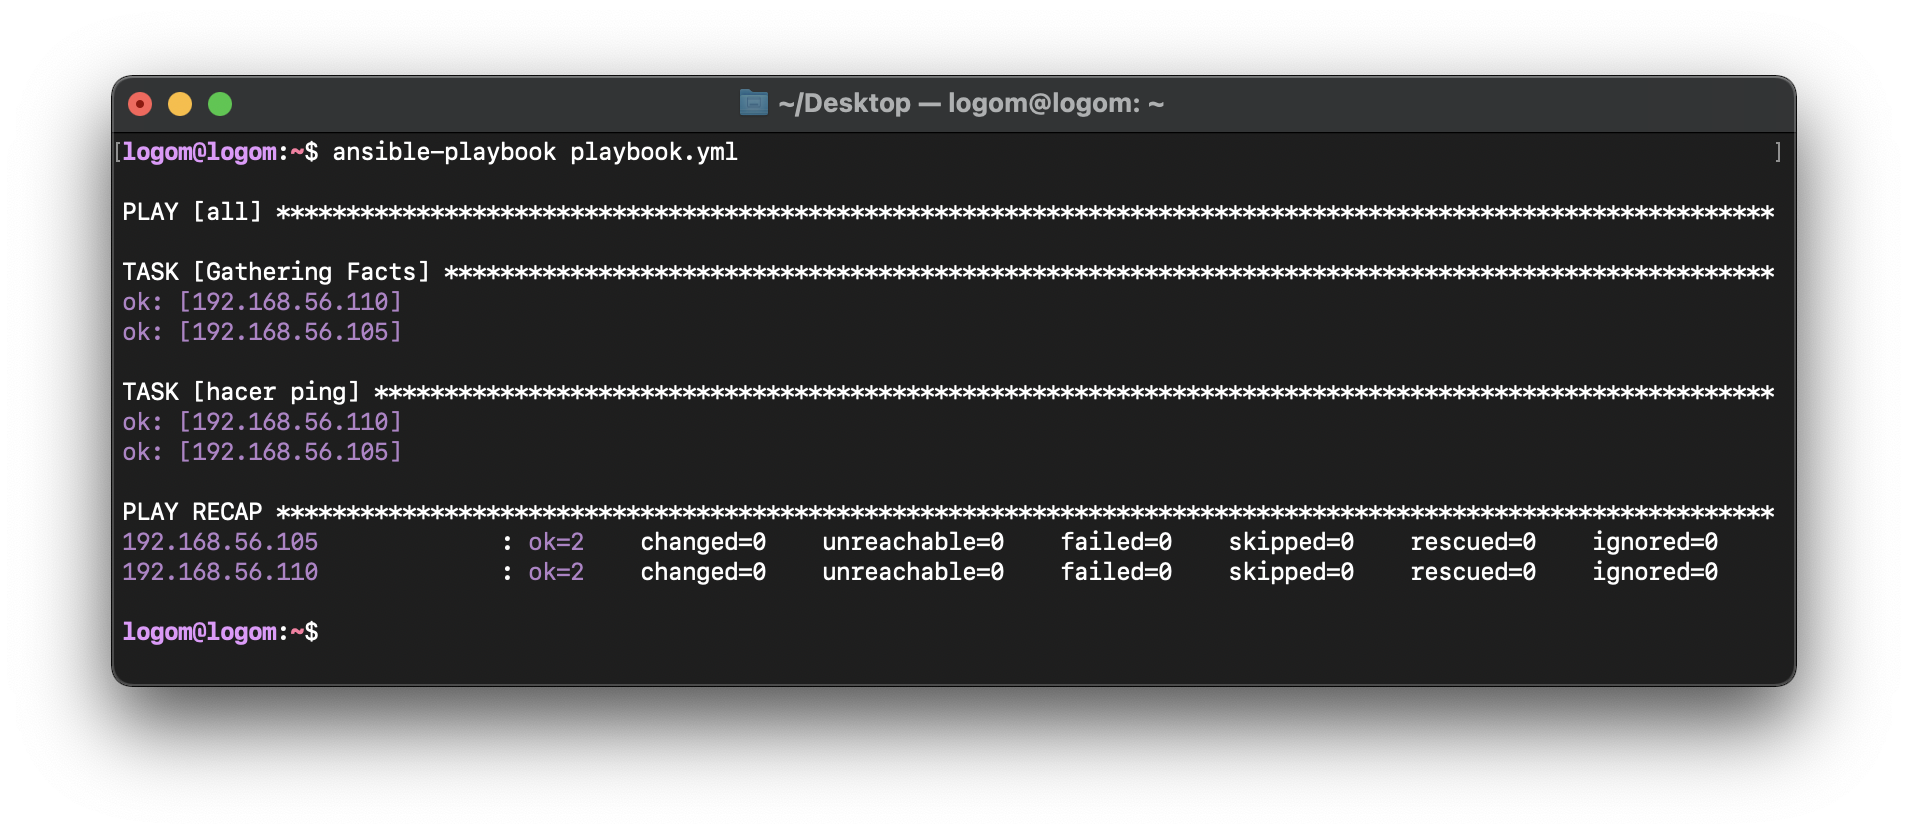
\includegraphics[scale=0.45]{images/ejecucion_playbook.png}
        \caption{Ejecución del playbook}
        \label{fig:ejecucion_playbook}
    \end{figure}

\begin{thebibliography}{0}
    \bibitem{} \href{https://www.zabbix.com/download?}{Zabbix download}
    \bibitem{} \href{https://www.zabbix.com/documentation/5.0/manual/installation/frontend}{Zabbix frontend installation}
    \bibitem{} \href{https://www.zabbix.com/documentation/5.4/en/manual/web_interface/frontend_sections/monitoring/dashboard/widgets}{Zabbix dashboard widgets}
    \bibitem{} \href{https://www.digitalocean.com/community/tutorials/how-to-install-and-configure-ansible-on-ubuntu-20-04-es}{How to install and configure ansible}
    \bibitem{} \href{https://www.youtube.com/watch?v=Wuv0ZPOMLf0}{How to do ansible playbooks}
\end{thebibliography}

\end{document}
